\documentclass[aspectratio=169]{beamer}

\usetheme{metropolis}

% ENCODING AND LANGUAGE
\usepackage[english]{babel}

\usepackage[utf8]{inputenc}     % Universal encoding
\usepackage[T1]{fontenc}        % Font encoding

% FONT
\usepackage{courier}            % Courier as \ttdefault
% \usepackage{psfrag}             % replace PostScript fonts

% OTHER HELPERS AND SETTINGS
% \usepackage{graphicx}           % Include graphics to document
% \usepackage{amsmath,amssymb,amstext}  % support for mathematics ttt

% \usepackage{listings}           % code listings
% \lstset{basicstyle=\footnotesize\ttfamily,breaklines=true}

% \usepackage{units}
\usepackage{siunitx}            % SI-Unit support

% TITLE PAGE SETTINGS
\title{Angel Introduction: Camera and Video Mixer}
% \date{\today \currenttime}
\author{}
\institute{C3VOC
	\begin{flushright}
		
\includegraphics[height=0.4\textheight]{images/link-repo-qr.png}\\
		https://github.com/voc/engelschulung
	\end{flushright}
}

%% START OF DOCUMENT
\begin{document}
\maketitle

% !TEX root = ../main.tex

\begin{frame}{General}
	\begin{itemize}
		\item We will stream, record and publish nearly all talks with your help
		\item You can operate the cameras and video mixer
		\item At do-not-record talks we also need angels % for guarding the camera or to do a recording, but no live stream
		\item We (people from c3voc) will be there to help
		\item The live stream video signal will also be the final recording
		\item We aim for consistent quality, but everybody make mistakes -- don't blame yourself!
	\end{itemize}
\end{frame}


\section{Angeltypes}
\begin{frame}{Angeltypes}
	\begin{itemize}
		\item A/V Angels:
		\begin{itemize}
			\item Camera Angels
			\item Video Mixer Angels
			\item Audio Mixer Angels
		\end{itemize}
		\item A/V Technician
		\item C3VOC Crew
%		\item External Crew % usually audio/light (remove roles above then)
%		\item Stage Manager
	\end{itemize}
\end{frame}

% !TEX root = ../main.tex

\begin{frame}{A/V Angel: Role Camera}
	\begin{itemize}
		\item One camera angel per camera in each lecture hall
		\item Operates the cameras in the lecture halls
		\item Maintains good camera settings
	\end{itemize}
\end{frame}

% !TEX root = ../main.tex

\begin{frame}{A/V Angel: Role Video Mixer}
	\begin{itemize}
		\item One person per lecture hall
		\item Operates the video mixer to produce an interesting video
		\begin{itemize}
			\item Switches between cameras and slides
			\item Composes pictures with multiple sources
			\item You decide, which sources to show
		\end{itemize}
		\item Mixed video feed is used for both, live-stream and the recordings 
		\item You might get assistance by a director on challenging talks
	\end{itemize}
\end{frame}

% !TEX root = ../main.tex

\begin{frame}{A/V Angel: Role Audio Mixer}
	\begin{itemize}
		\item This might also be the task of the video mixing angel
		\item Mute and un-mute microphones when they are used/ not used
		\item Change the amplification for individual microphones
		\item Check the audio level (loudness) for stream
	\end{itemize}
\end{frame}

% !TEX root = ../main.tex

\begin{frame}{C3VOC Crew}
	\begin{itemize}
		\item 2nd to n-th level support in the lecture halls.
		\item Responsible for keeping stuff working
		\item Familiar with all equipment in use
		\item Able to fix (nearly) all the issues
		\item Reachable via phone/ DECT
	\end{itemize}
\end{frame}

%% !TEX root = ../main.tex

\begin{frame}{External Crew}
	\begin{itemize}
		\item Does audio mixing and controls the lighting fixtures.
		\item Ensures that the stage and their equipment works
		\item Please refrain from bothering them all the time
        \item Ask A/V Tech first
		\item They are still nice people
	\end{itemize}
\end{frame}

% !TEX root = ../main.tex

\begin{frame}{A/V Technician}
	\begin{itemize}
		\item Direct support for you in the lecture hall
		\item Makes sure, that speaker laptop is connected
		\item Responsible for the speaker's headset microphone
		\item Communication gateway to the Stage Managers and external crew
		\item Your \textbf{first contact for any technical issues} in the lecture hall
		\item Shifts usually last four hours
	\end{itemize}
\end{frame}

%% !TEX root = ../main.tex

\begin{frame}{Stage Manager}
	\begin{itemize}
		\item Is responsible for the lecture hall operations:
		\begin{itemize}
			\item Cooridnation with all teams (VOC, Heralds, Translation, etc.)
			\item Crowd control
			\item Time keeping
			\item Last minute issues
		\end{itemize}
		\item Carries the radio for emergency communication
		\item Same shift schedule as the A/V-Technicians
	\end{itemize}
\end{frame}



\section{Basics}
% !TEX root = ../main.tex

\begin{frame}{Closeup Shot}
	\begin{itemize}
		\item Show the head and upper part of the body
		\item Leave the width of one hand above the head
		\item Eyes should be close to the upper third line
	\end{itemize}
\end{frame}

\begin{frame}{Closeup Shot: Good Example}
	\begin{figure}
		\centering
		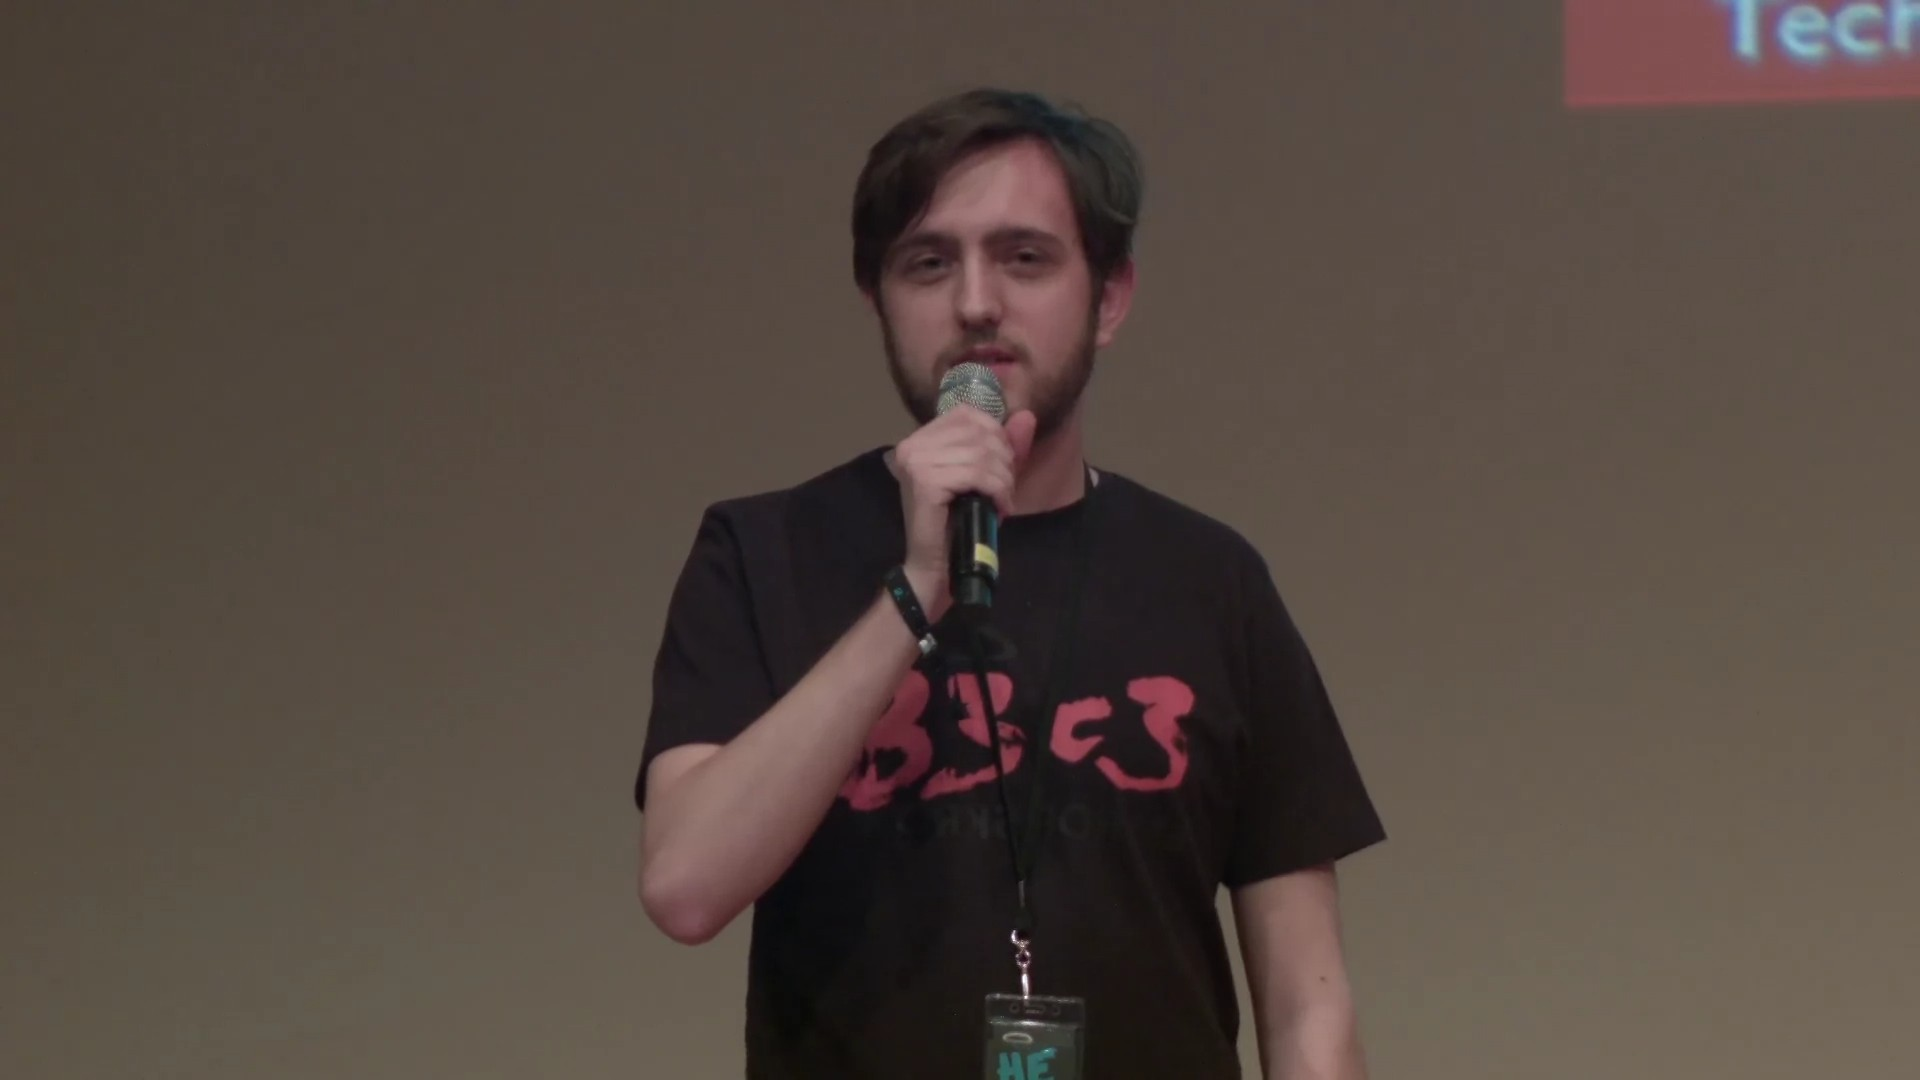
\includegraphics[width=0.75\textwidth]{images/shot-closeup1.jpg}
		\caption{Good closeup shot}
	\end{figure}
\end{frame}

% TODO: Replace with a screenshot from voctomix 2
\begin{frame}{Closeup Shot: Good Example}
	\begin{figure}
		\centering
		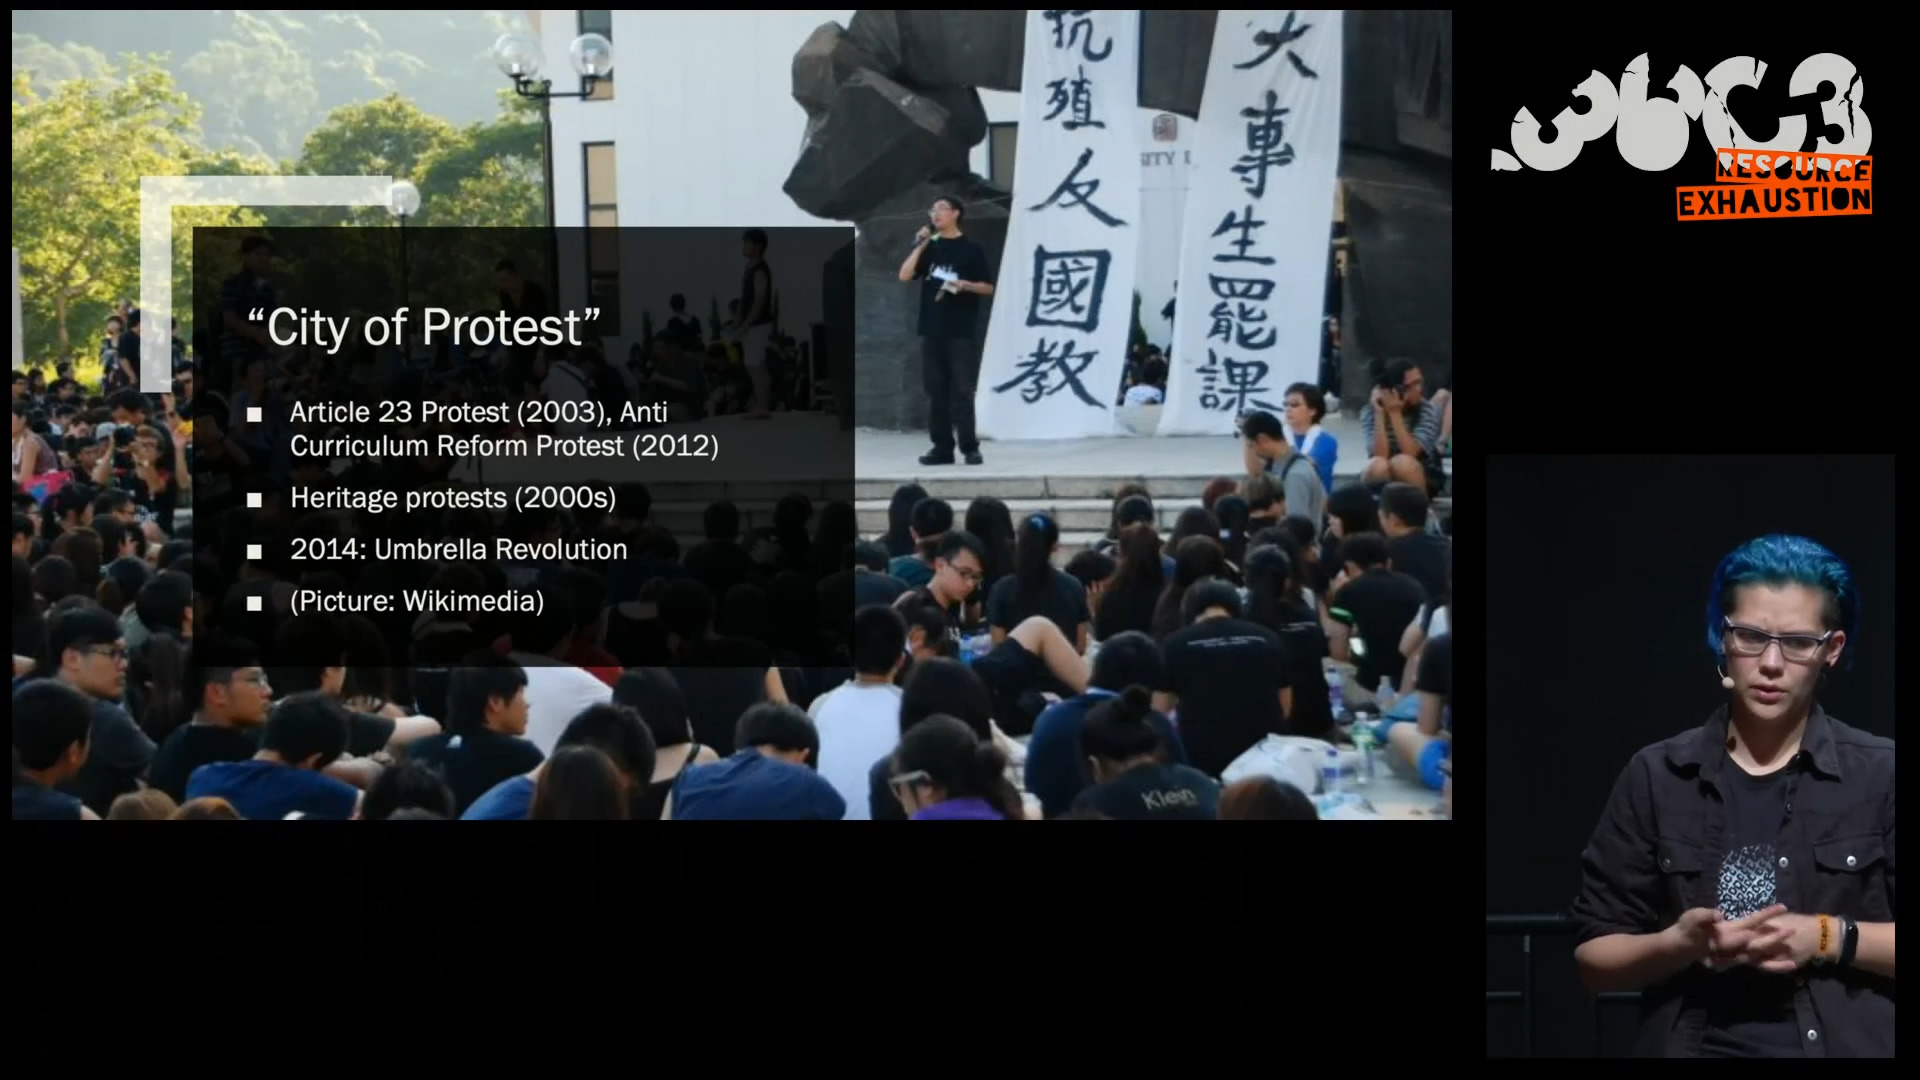
\includegraphics[width=0.75\textwidth]{images/shot-closeup2.jpg}
		\caption{Good closeup in Lecture Mode}
	\end{figure}
\end{frame}

\begin{frame}{Closeup Shot: Bad Example}
	\begin{figure}
		\centering
		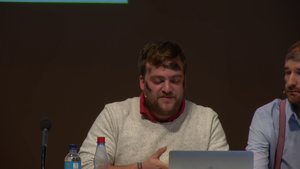
\includegraphics[width=0.75\textwidth]{images/shot-closeup-bad1.png}
		\caption{Half a head - not good}
	\end{figure}
\end{frame}

\begin{frame}{Closeup Shot: Bad Example}
	\begin{figure}
		\centering
		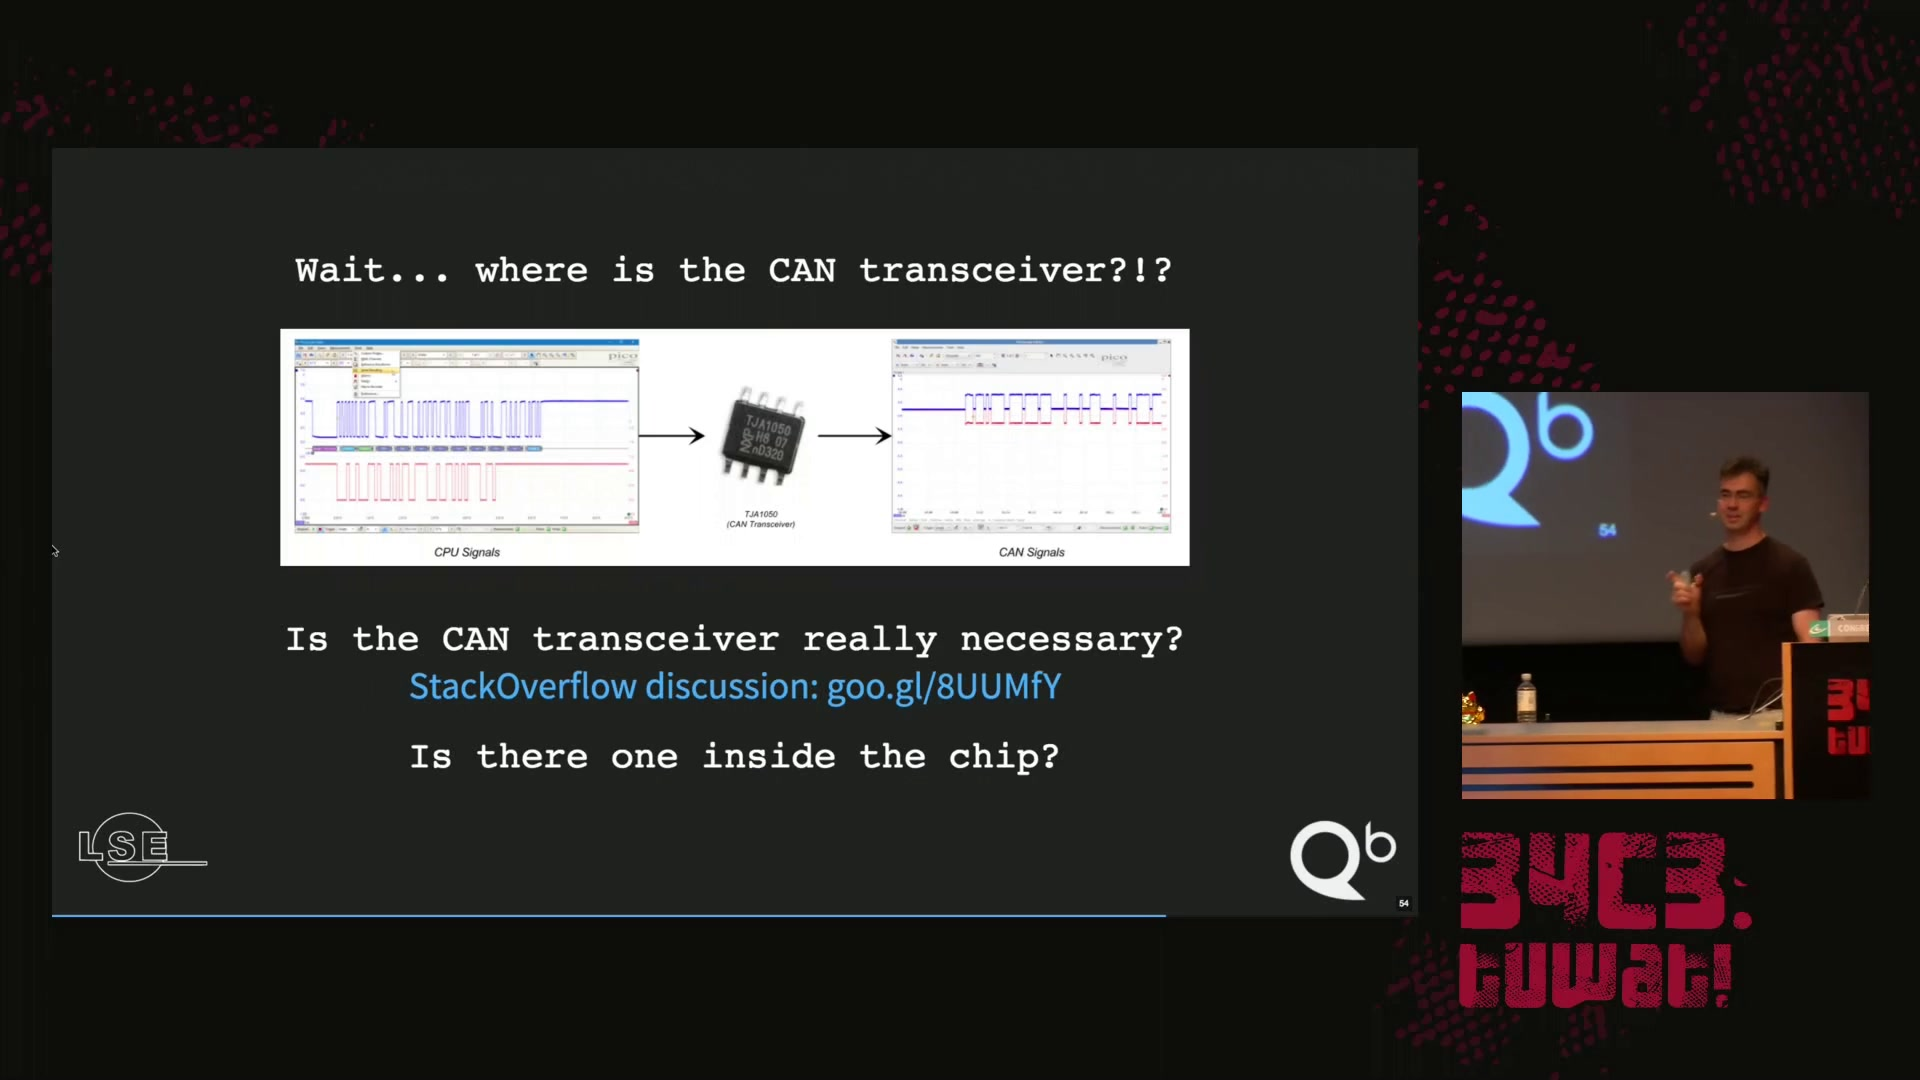
\includegraphics[width=0.75\textwidth]{images/shot-closeup-bad2.png}
		\caption{Too far out for a good Lecture Mode image}
	\end{figure}
\end{frame}

\begin{frame}{Medium Shot: Good 1}
	\begin{figure}
		\centering
		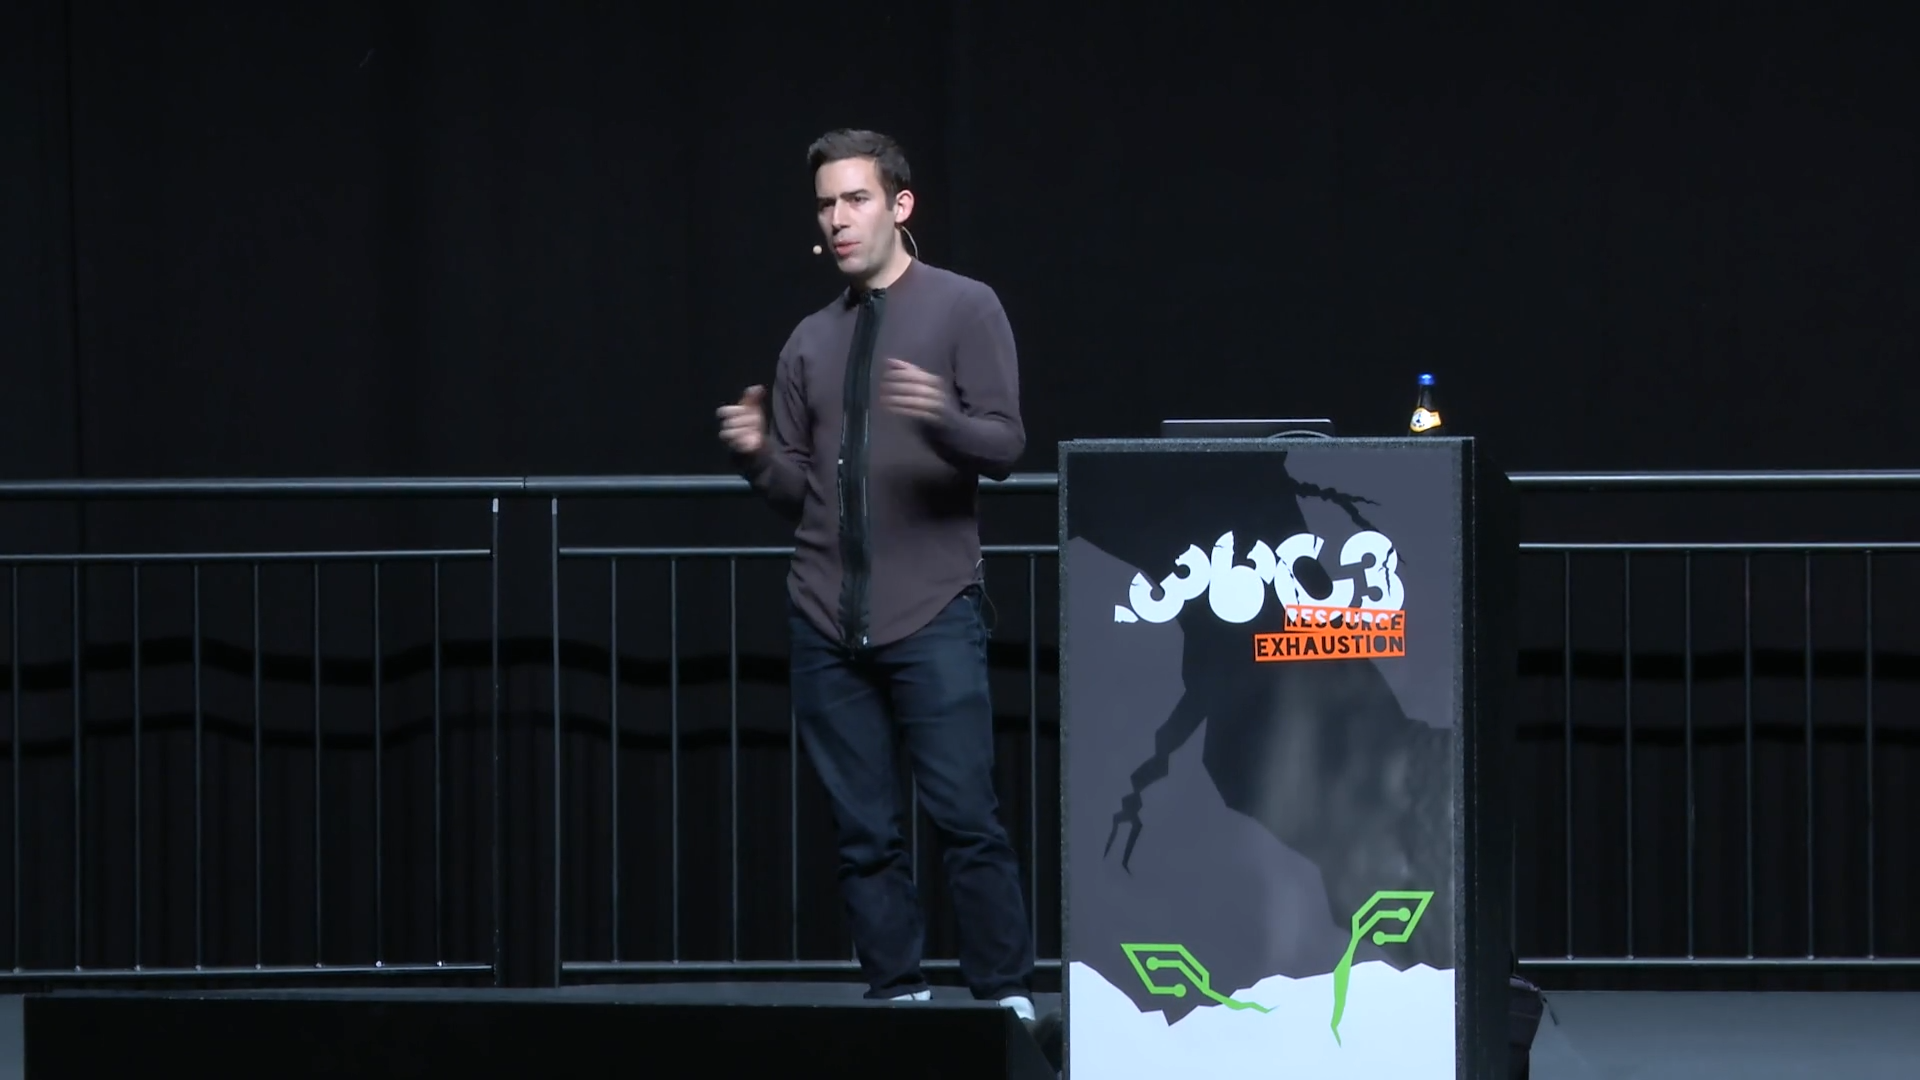
\includegraphics[width=0.75\textwidth]{images/shot-medium1.png}
		\caption{One person, the lectern and some context}
	\end{figure}
\end{frame}

\begin{frame}{Medium Shot: Good 2}
	\begin{figure}
		\centering
		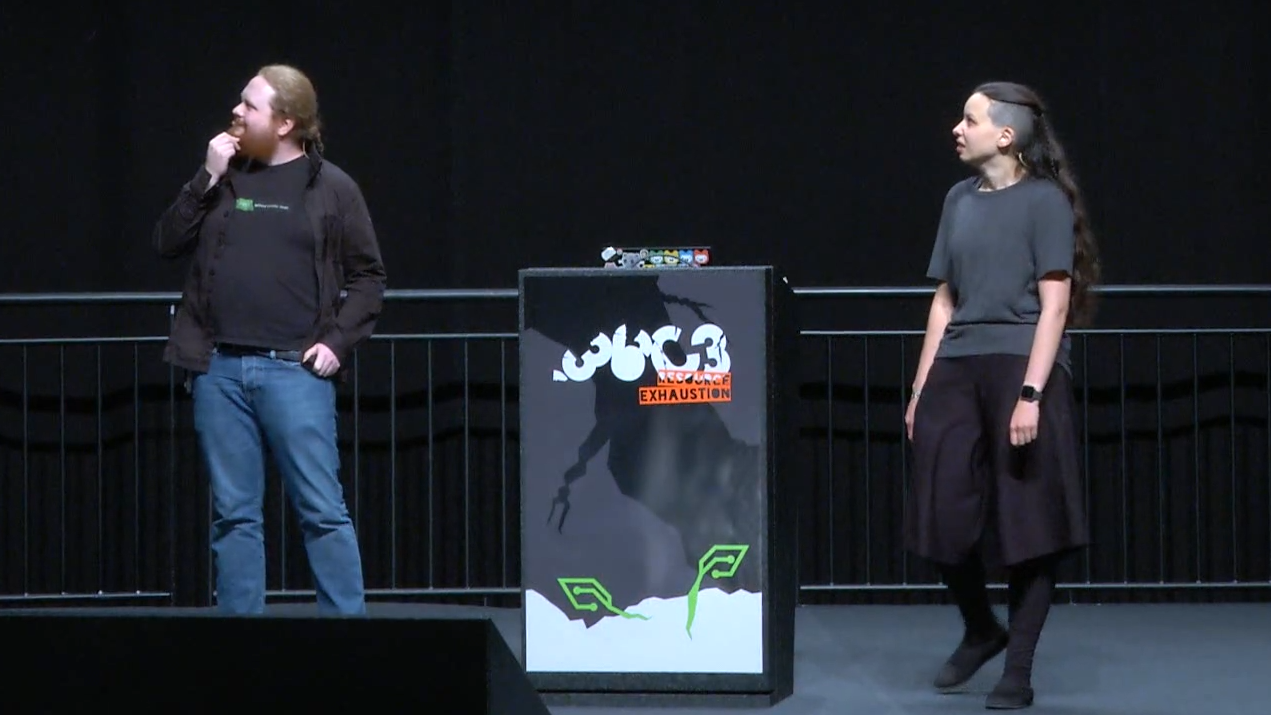
\includegraphics[width=0.75\textwidth]{images/shot-medium2.png}
		\caption{Two persons on stage}
	\end{figure}
\end{frame}

\begin{frame}{Overview}
	\begin{itemize}
		\item Shows the complete stage and the people on it
		\item Heads of the crowd are OK, if it's dark enough
		\item Don't use this camera to show the slides - use lecture mode instead
		\item Locked off, do not move.
	\end{itemize}
\end{frame}

\begin{frame}{Wide Shot: Good Example}
	\begin{figure}
		\centering
		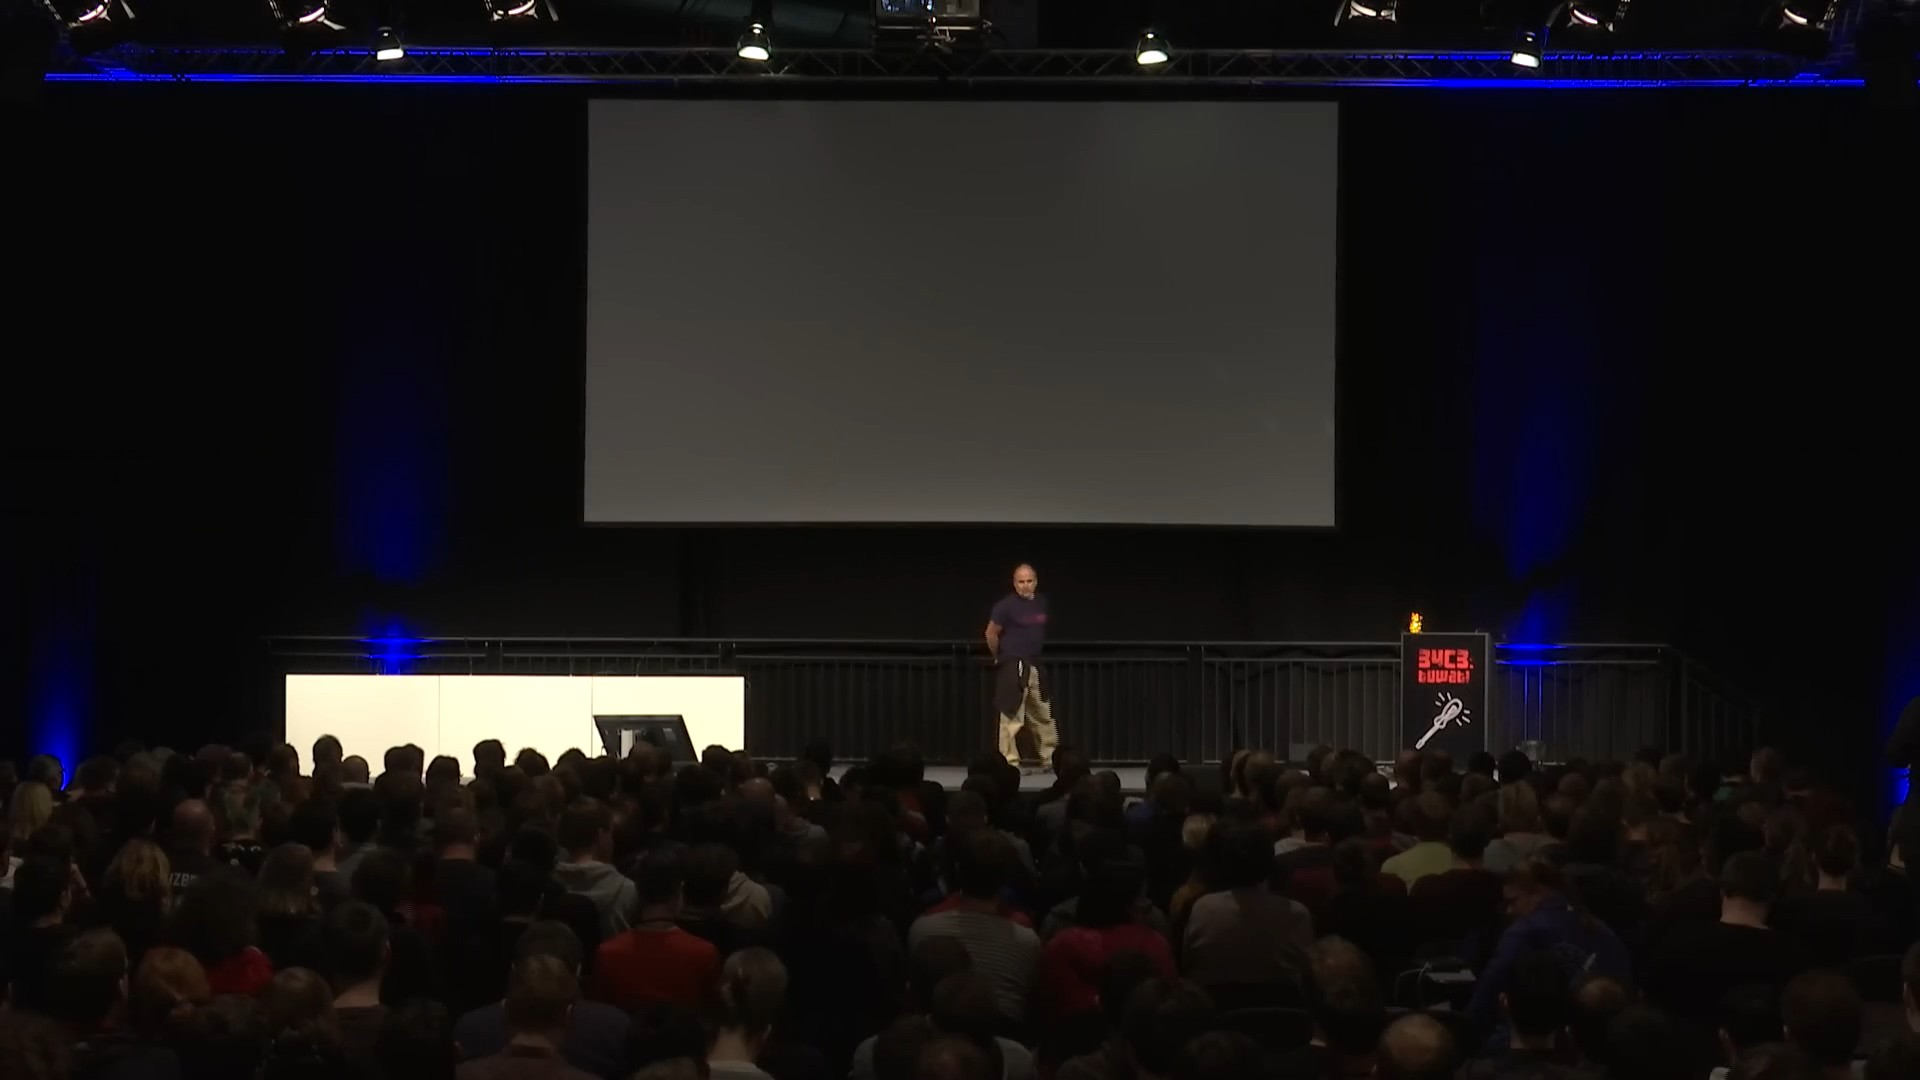
\includegraphics[width=0.75\textwidth]{images/shot-wide.jpeg}
	\end{figure}
\end{frame}


\begin{frame}{Usual Talk Timeline}
  \begin{itemize}
    \item Please be on time when your shift starts
    \item Get to know your fellow angels, check the camera and mixer
    \item Talk starts with an introduction by the herald
    \item Speaker starts talk
    \item Q\&A session
    \item Talk ends with "thank you" and applause
    \item Hand over to the next angels
  \end{itemize}
\end{frame}

%% !TEX root = ../main.tex

\begin{frame}{Timeline - Preparations}
	\begin{block}{Camera}
		\begin{itemize}
			\item Test your camera and tripod
			\item Check who is herald and speaker
			\item Show the stage, ideally with herald and speaker
		\end{itemize}
	\end{block}
	\begin{block}{Mixer}
		\begin{itemize}
			\item Be prepared to go live
			\item Signal that you're ready when the talk should start
		\end{itemize}
	\end{block}
\end{frame}

\begin{frame}{Timeline - Introduction}
	\begin{block}{Camera}
		\begin{itemize}
			\item Follow the herald, if necessary
		\end{itemize}
	\end{block}
	\begin{block}{Mixer}
		\begin{itemize}
			\item Show the herald (and speaker)
			\item Put fullscreen slides on preview
			\item Switch to slides when announcement is finished
		\end{itemize}
	\end{block}
\end{frame}

\begin{frame}{Timeline - Content}
	\begin{block}{Camera}
		\begin{itemize}
			\item Show closeup of the speaker
			\item Follow the speaker, if necessary
		\end{itemize}
	\end{block}
	\begin{block}{Mixer}
		\begin{itemize}
			\item Show new slides as soon as they are keyed by the Speaker 
			\item Show slides long enough (read slide 2 times)
			\item Use lecture mode, if possible
			\item Use the camera in fullscreen, if there's action on the stage
			\item Try to plan ahead and anticipate the next actions by the speaker
		\end{itemize}
	\end{block}
\end{frame}

\begin{frame}{Timeline - Questions and Answers}
	\begin{block}{Cameras}
		\begin{itemize}
			\item Camera: Track the Speaker
			\item Keep tracking, don't give up even if your shift ends soon
		\end{itemize}
	\end{block}
	\begin{block}{Mixer}
		\begin{itemize}
			\item Show whoever is talking on stage to the stream
			\item The "Thanks"-Slide can be shown from time to time
			\item Don't end too early
		\end{itemize}
	\end{block}
\end{frame}

%% !TEX root = ../main.tex

\begin{frame}{Timeline - Preparations}
	\begin{block}{Cameras}
		\begin{itemize}
			\item Test your camera and tripod
			\item Check who is herald and speaker
			\item Camera 1: Get a closeup of the speaker
			\item Camera 2: Show the stage, ideally with herald and speaker
		\end{itemize}
	\end{block}
	\begin{block}{Mixer}
		\begin{itemize}
			\item Have camera 2 on program and be prepared to go live
			\item Signal that you're ready when the talk should start
		\end{itemize}
	\end{block}
\end{frame}

\begin{frame}{Timeline - Introduction}
	\begin{block}{Cameras}
		\begin{itemize}
			\item Cam 1: Follow the speaker, if necessay
			\item Cam 2: Keep the herald in frame
		\end{itemize}
	\end{block}
	\begin{block}{Mixer}
		\begin{itemize}
			\item Go live with Camera 2 as soon as the Herald starts
			\item Title slide can be shown during the introduction 
			\item Be prepared to switch to Lecture Mode or Camera 1 as soon as the speaker starts talking
		\end{itemize}
	\end{block}
\end{frame}

\begin{frame}{Timeline - Content}
	\begin{block}{Cameras}
		\begin{itemize}
			\item With intercom: Follow commands from your mixer and ask for time off, if you need to re-adjust something
			\item Cam 1: Follow the speaker with a closeup shot
			\item Cam 2: Get a medium shot of the speaker (for gestures and walking around)
		\end{itemize}
	\end{block}
	\begin{block}{Mixer}
		\begin{itemize}
			\item Show new slides as soon as they are keyed by the Speaker 
			\item Show slides long enough (read slide 2 times)
			\item Use lecture mode, if possible
			\item Use the camera in fullscreen, if there's action on the stage
			\item Try to plan ahead and anticipate the next actions by the speaker
		\end{itemize}
	\end{block}
\end{frame}

\begin{frame}{Timeline - Questions and Answers}
	\begin{block}{Cameras}
		\begin{itemize}
			\item Cam 1: Track the Speaker
			\item Cam 2: Show the herald as well
			\item Keep tracking, don't give up even if your shift ends soon
		\end{itemize}
	\end{block}
	\begin{block}{Mixer}
		\begin{itemize}
			\item Show whoever is talking on stage to the stream
			\item The "Thanks"-Slide can be shown from time to time
			\item Don't end too early
		\end{itemize}
	\end{block}
\end{frame}



\section{Camera Hardware}
% !TEX root = ../main.tex

\begin{frame}{Hardware Camera Controls Panasonic}
	\begin{columns}[T,onlytextwidth]
		\column{0.5\textwidth}
	\begin{figure}
		\centering
		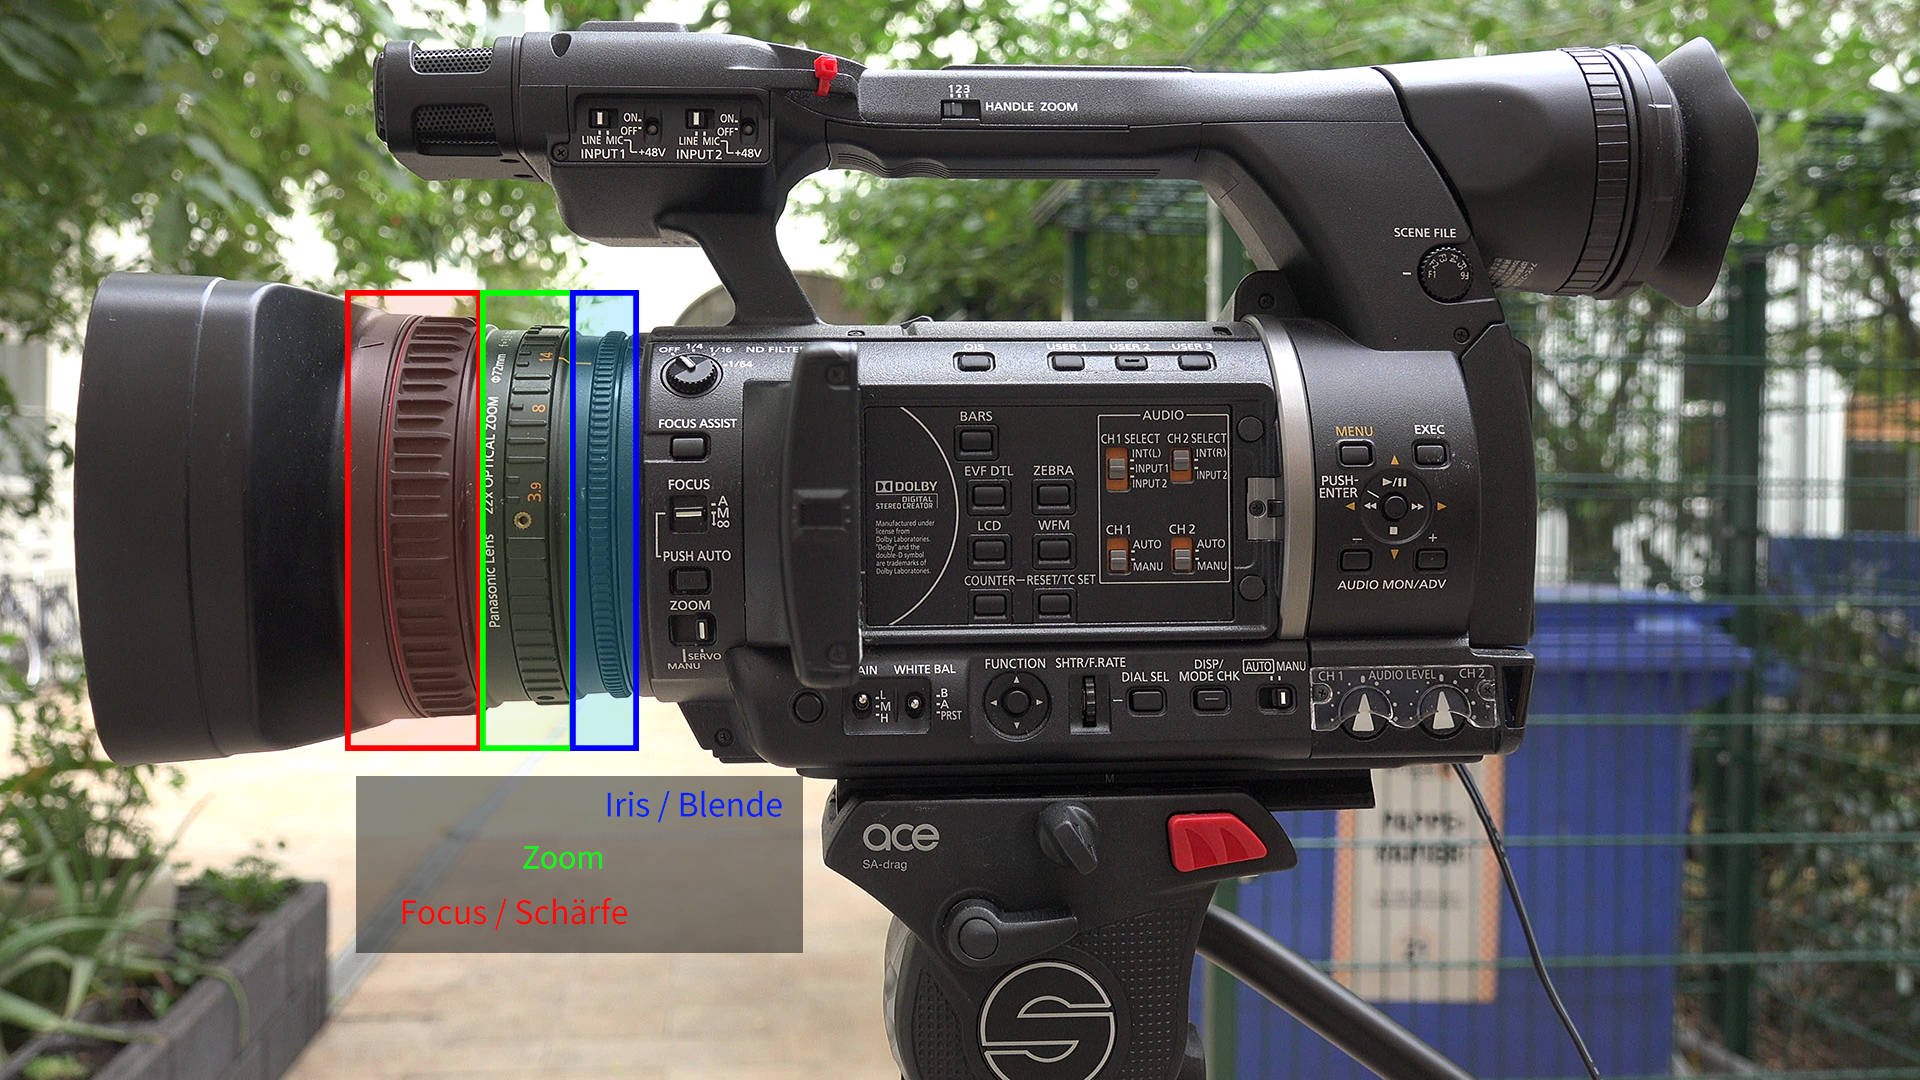
\includegraphics[width=0.9\textwidth]{images/panasonic-side-annotated.jpg}
		\caption{Panasonic Cam}
	\end{figure}
		\column{0.5\textwidth}
		Cameras are in manual mode because of difficult lighting situation.
		\begin{description}
			\item[Left Ring/red] Focus - control sharpness of the image.
			\item[Middle Ring/green] Zoom - vary the focal length.
			\item[Right Ring/blue] Iris - will have to be adjusted throughout the day. If there is anything wrong, contact C3VOC helpdesk.
		\end{description}
	\end{columns}
\end{frame}

\begin{frame}{Zoom Control Panasonic}
	\begin{columns}[T,onlytextwidth]
		\column{0.5\textwidth}
	\begin{figure}
		\centering
		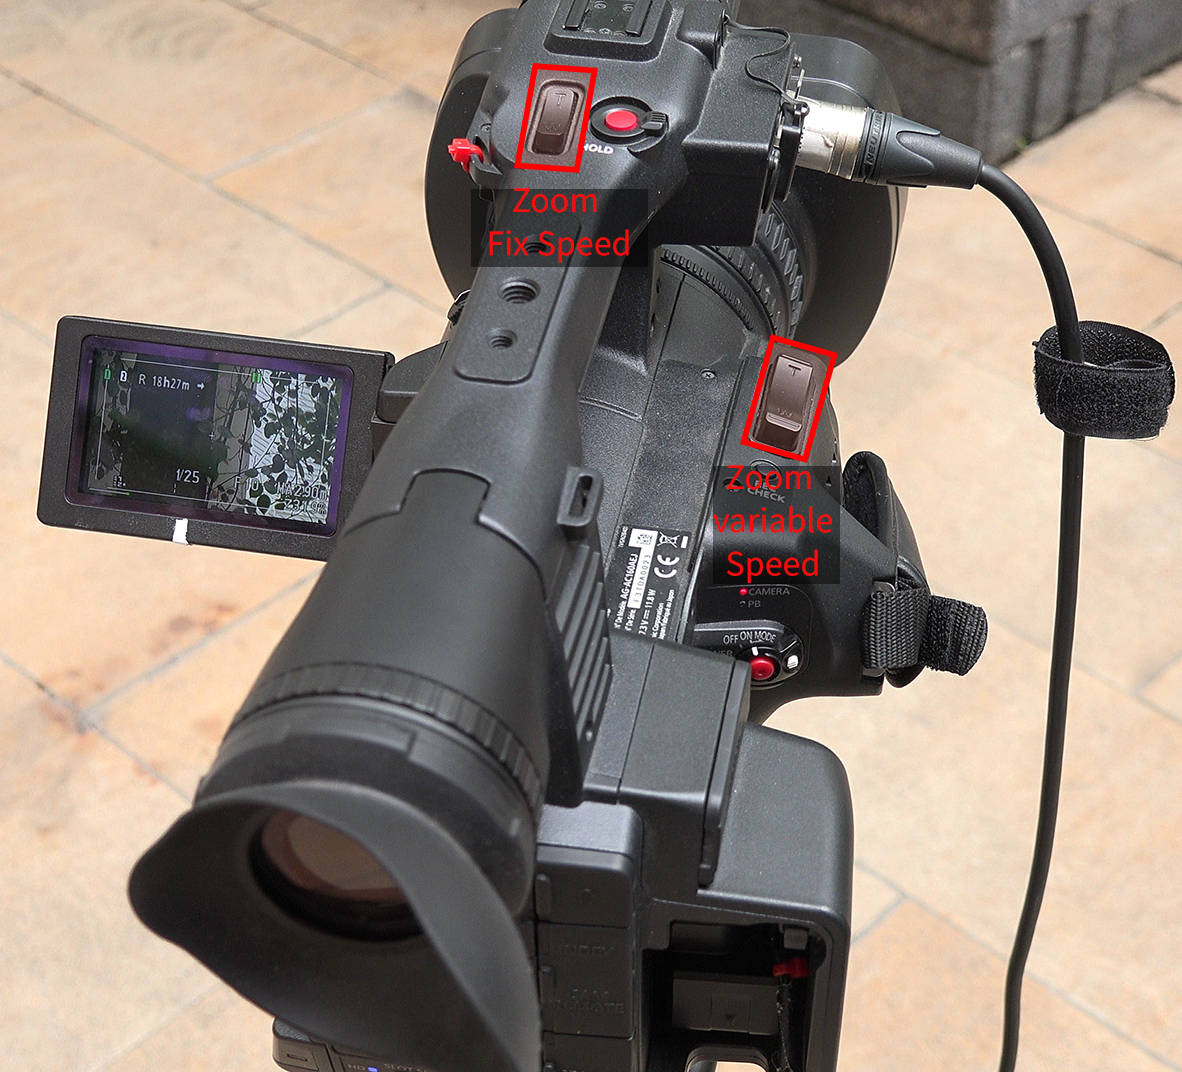
\includegraphics[width=0.99\textwidth]{images/panasonic-zoom-annotated.jpg}
		\caption{Panasonic Cam}
	\end{figure}
		\column{0.5\textwidth}
		\begin{itemize}
			\item For smooth zoom use the zoom buttons.
			\item Gentle touch $\Rightarrow$ slow zoom
			\item Top Buttons fixed speed
		\end{itemize}
	\end{columns}
\end{frame}

\begin{frame}{Display Indicators Panasonic}
	\begin{columns}[T,onlytextwidth]
		\column{0.5\textwidth}
	\begin{figure}
		\centering
		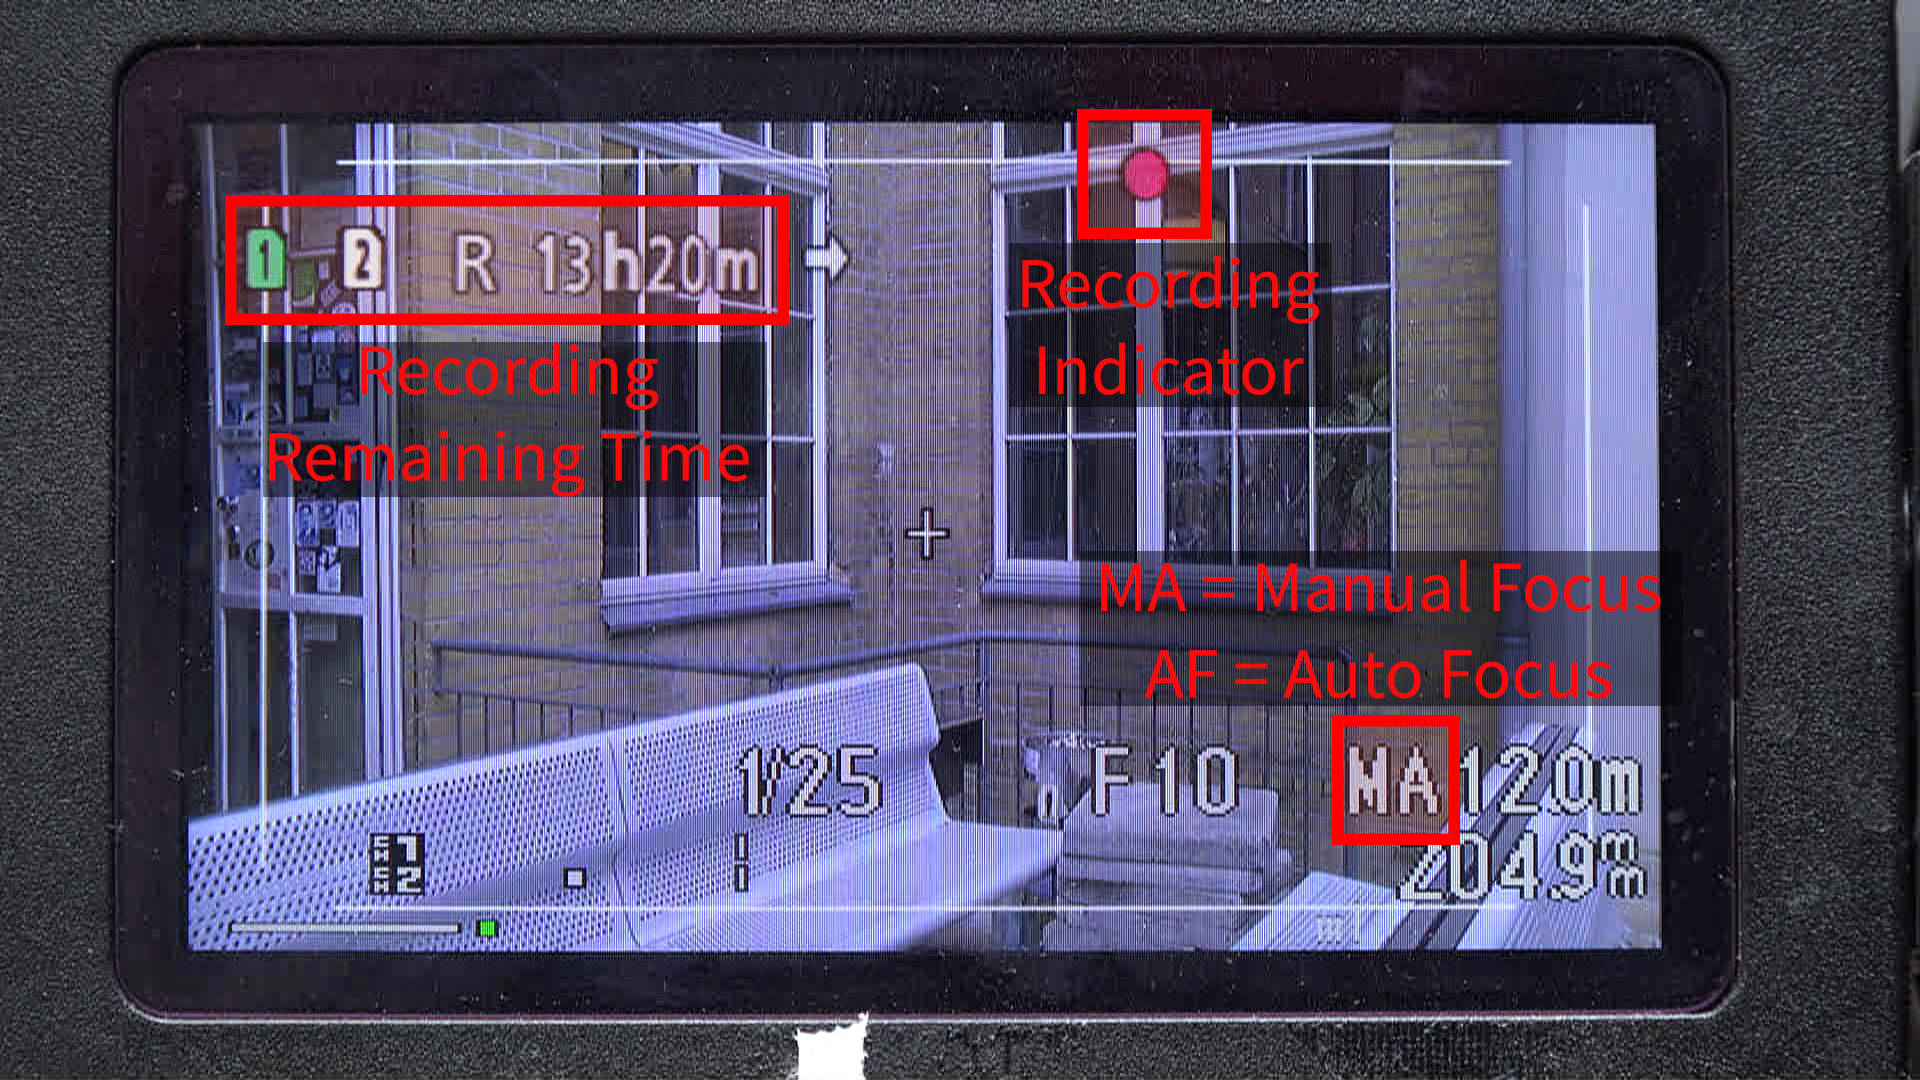
\includegraphics[width=0.9\textwidth]{images/panasonic-display-annotated.jpg}
		\caption{Panasonic Display Indicators}
	\end{figure}
		\column{0.5\textwidth}
		\begin{description}
			\item[Rec Indicator] The recording must always run, even during the break.
			\item[Focal Indicator] Use only manual focus!
			\item[Remaining Time] It must have enough remaing time before talk.
		\end{description}
		\metroset{block=fill}
		\begin{alertblock}{Alert}
			Alert the A/V-Technician if something's wrong.
		\end{alertblock}
	\end{columns}
\end{frame}

% !TEX root = ../main.tex

\begin{frame}{Hardware Camera Controls Sony PXW-Z200}
	\begin{columns}[T,onlytextwidth]
		\column{0.5\textwidth}
	\begin{figure}
		\centering
		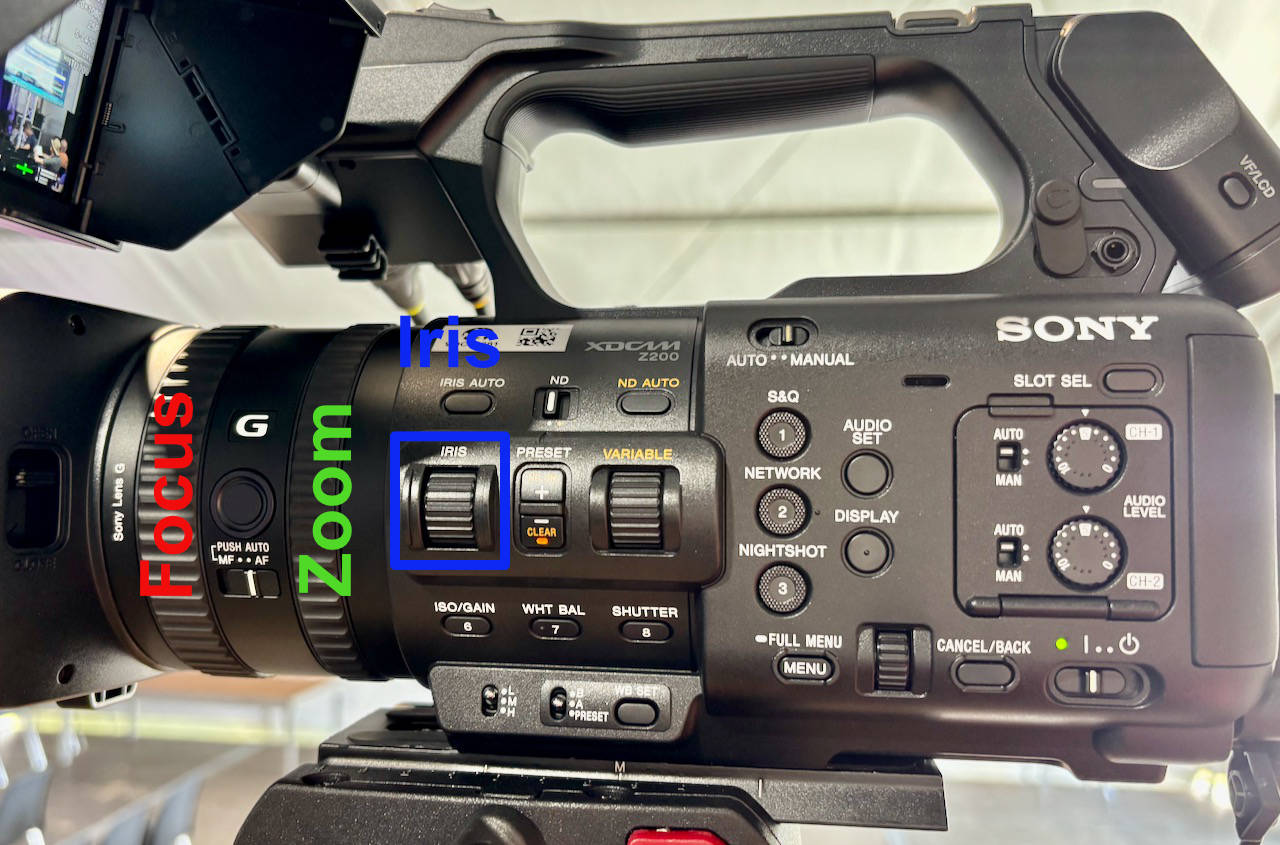
\includegraphics[width=0.9\textwidth]{images/sony-side-annotated.jpg}
		\caption{Sony Cam}
	\end{figure}
		\column{0.5\textwidth}
		Cameras are in manual mode because of difficult lighting situation.
		\begin{description}
			\item[Left Ring/red] Focus - control sharpness of the image.
			\item[MF/AF Selector] Auto Focus - always on.
			\item[Middle Ring/green] Zoom - vary the focal length.
			\item[Right Ring/blue] Iris - adjust according to lighting situation.
		\end{description}
	\end{columns}
  If there is anything wrong, contact C3VOC helpdesk.
\end{frame}

\begin{frame}{Zoom Control Sony}
	\begin{columns}[T,onlytextwidth]
		\column{0.5\textwidth}
	\begin{figure}
		\centering
		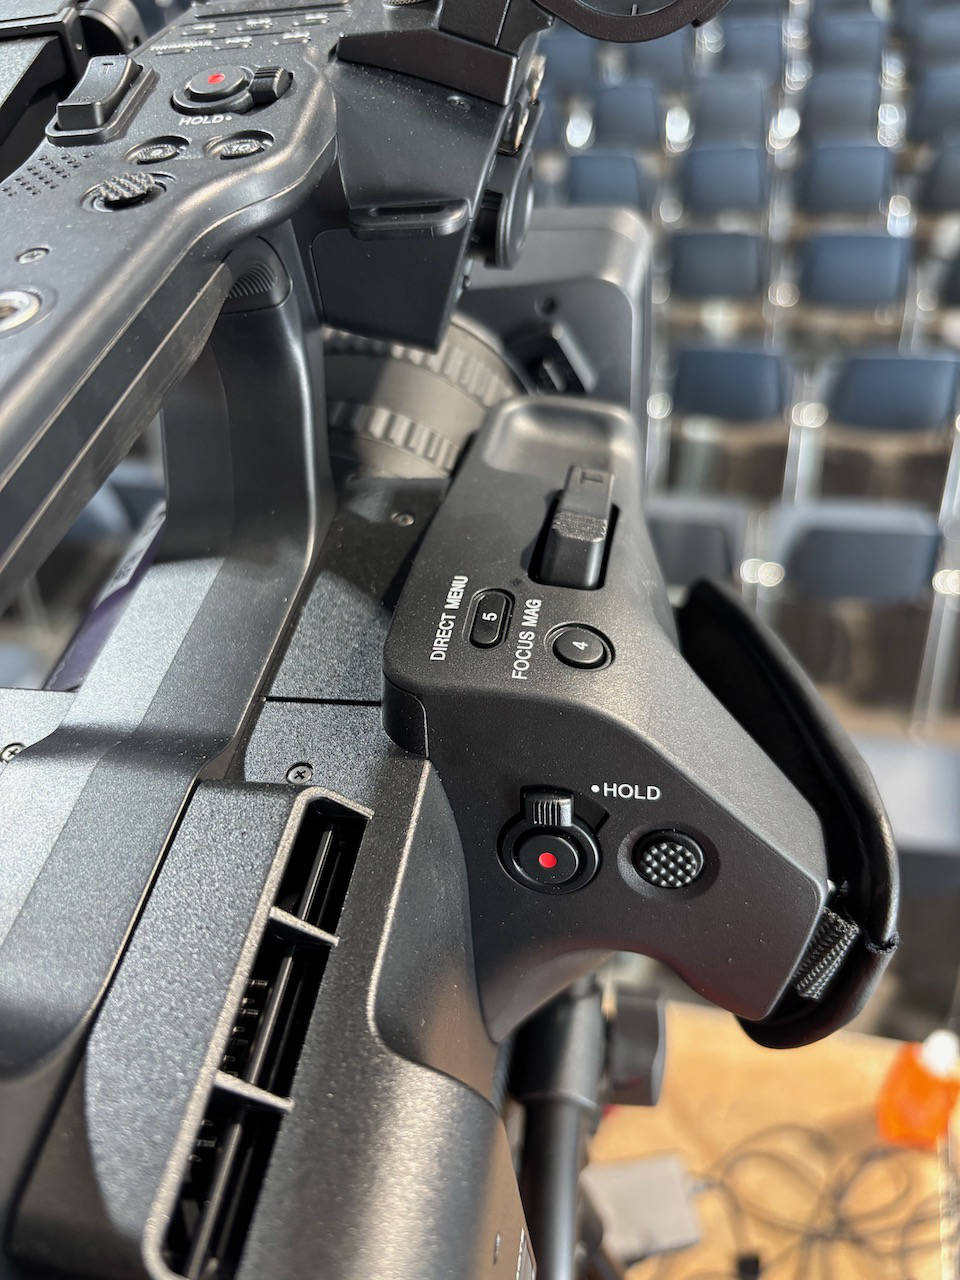
\includegraphics[width=0.99\textwidth]{images/sony-zoom.jpg}
		\caption{Sony Cam}
	\end{figure}
		\column{0.5\textwidth}
		\begin{itemize}
			\item For smooth zoom use the zoom buttons.
			\item Gentle touch $\Rightarrow$ slow zoom
		\end{itemize}
	\end{columns}
\end{frame}

\begin{frame}{Display Indicators Sony}
	\begin{columns}[T,onlytextwidth]
		\column{0.5\textwidth}
	\begin{figure}
		\centering
		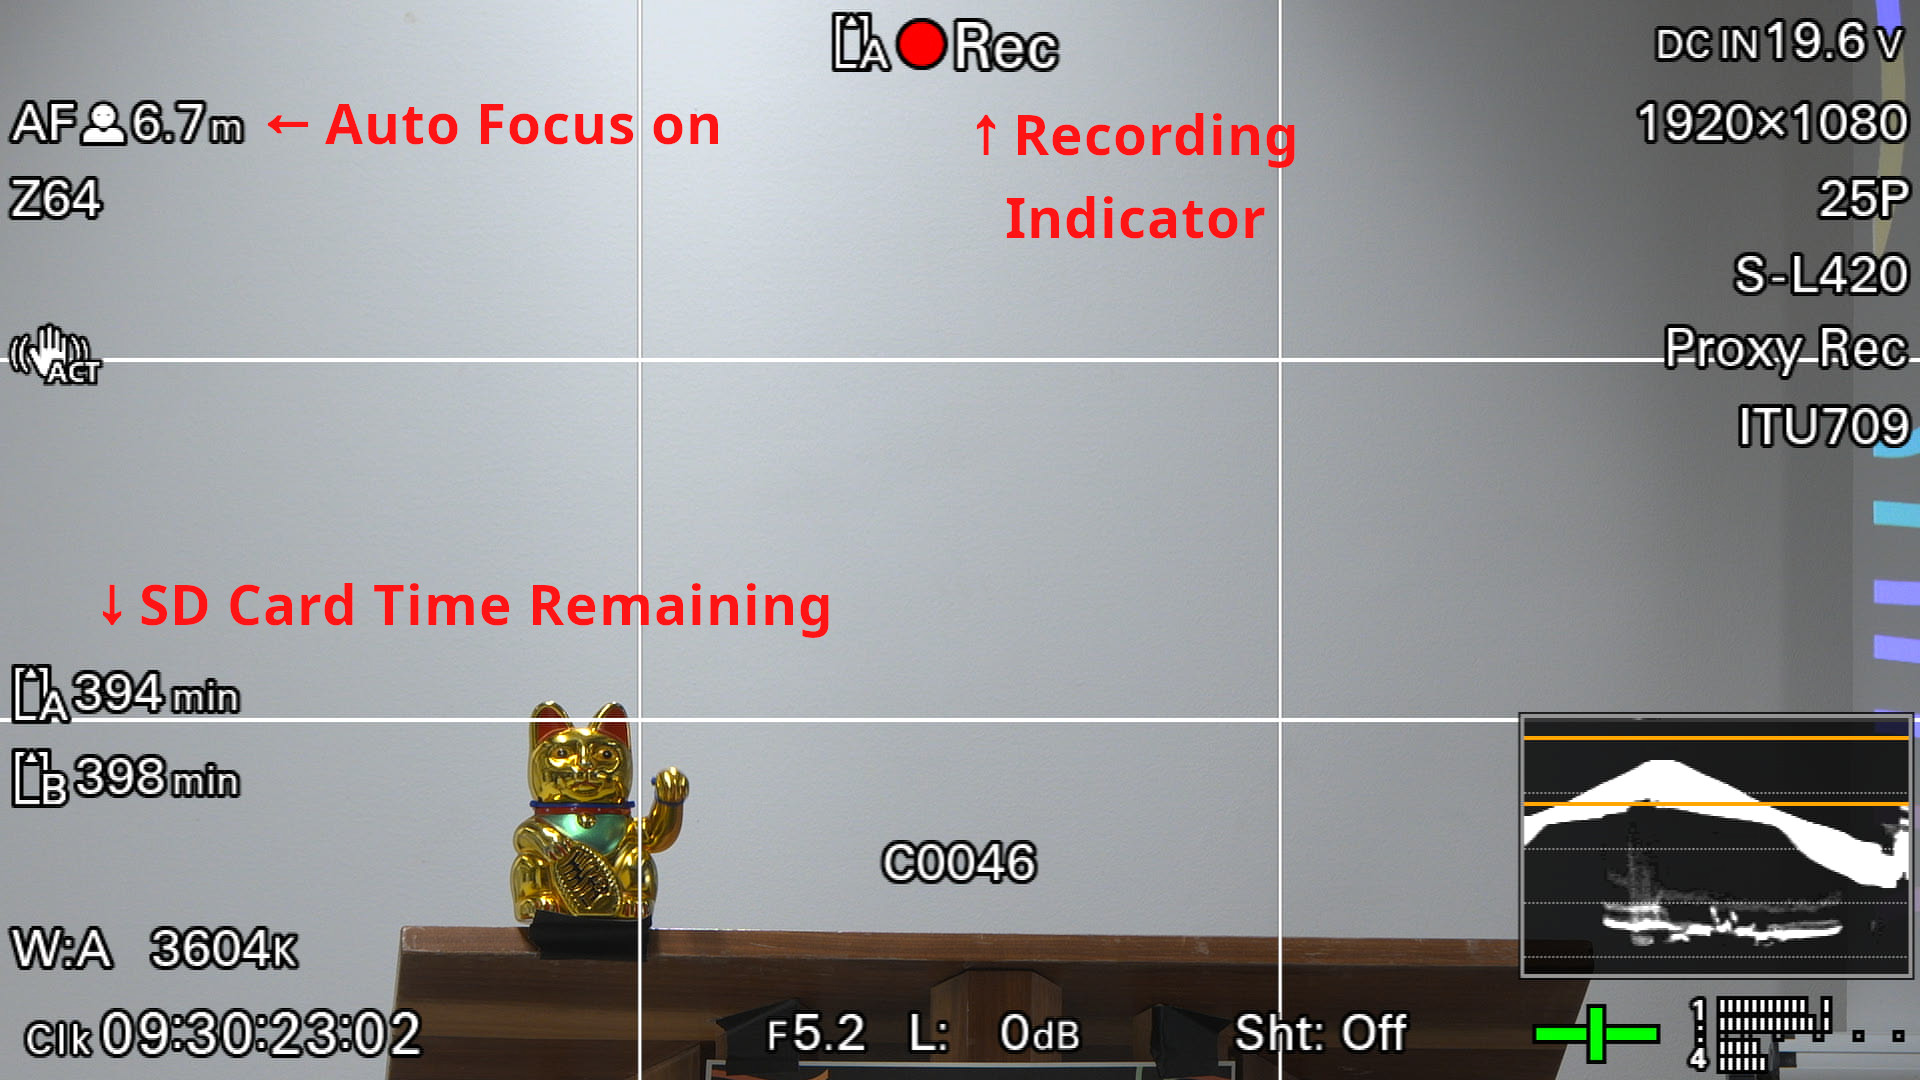
\includegraphics[width=0.9\textwidth]{images/sony-display-description.jpg}
		\caption{Sony Display Indicators}
	\end{figure}
		\column{0.5\textwidth}
		\begin{description}
			\item[Focal Indicator] Autofocus with face tracking is awesome!
			\item[Rec Indicator] The recording must always run, even during the break.
			\item[Remaining Time] More minutes remaining than the length of the next talk.
		\end{description}
		\metroset{block=fill}
		\begin{alertblock}{Alert}
			Alert the A/V-Technician if something's wrong.
		\end{alertblock}
	\end{columns}
\end{frame}

%% !TEX root = ../main.tex

\begin{frame}{Hardware Camera Controls JVC}
	\begin{columns}[T,onlytextwidth]
		\column{0.5\textwidth}
	\begin{figure}
		\centering
		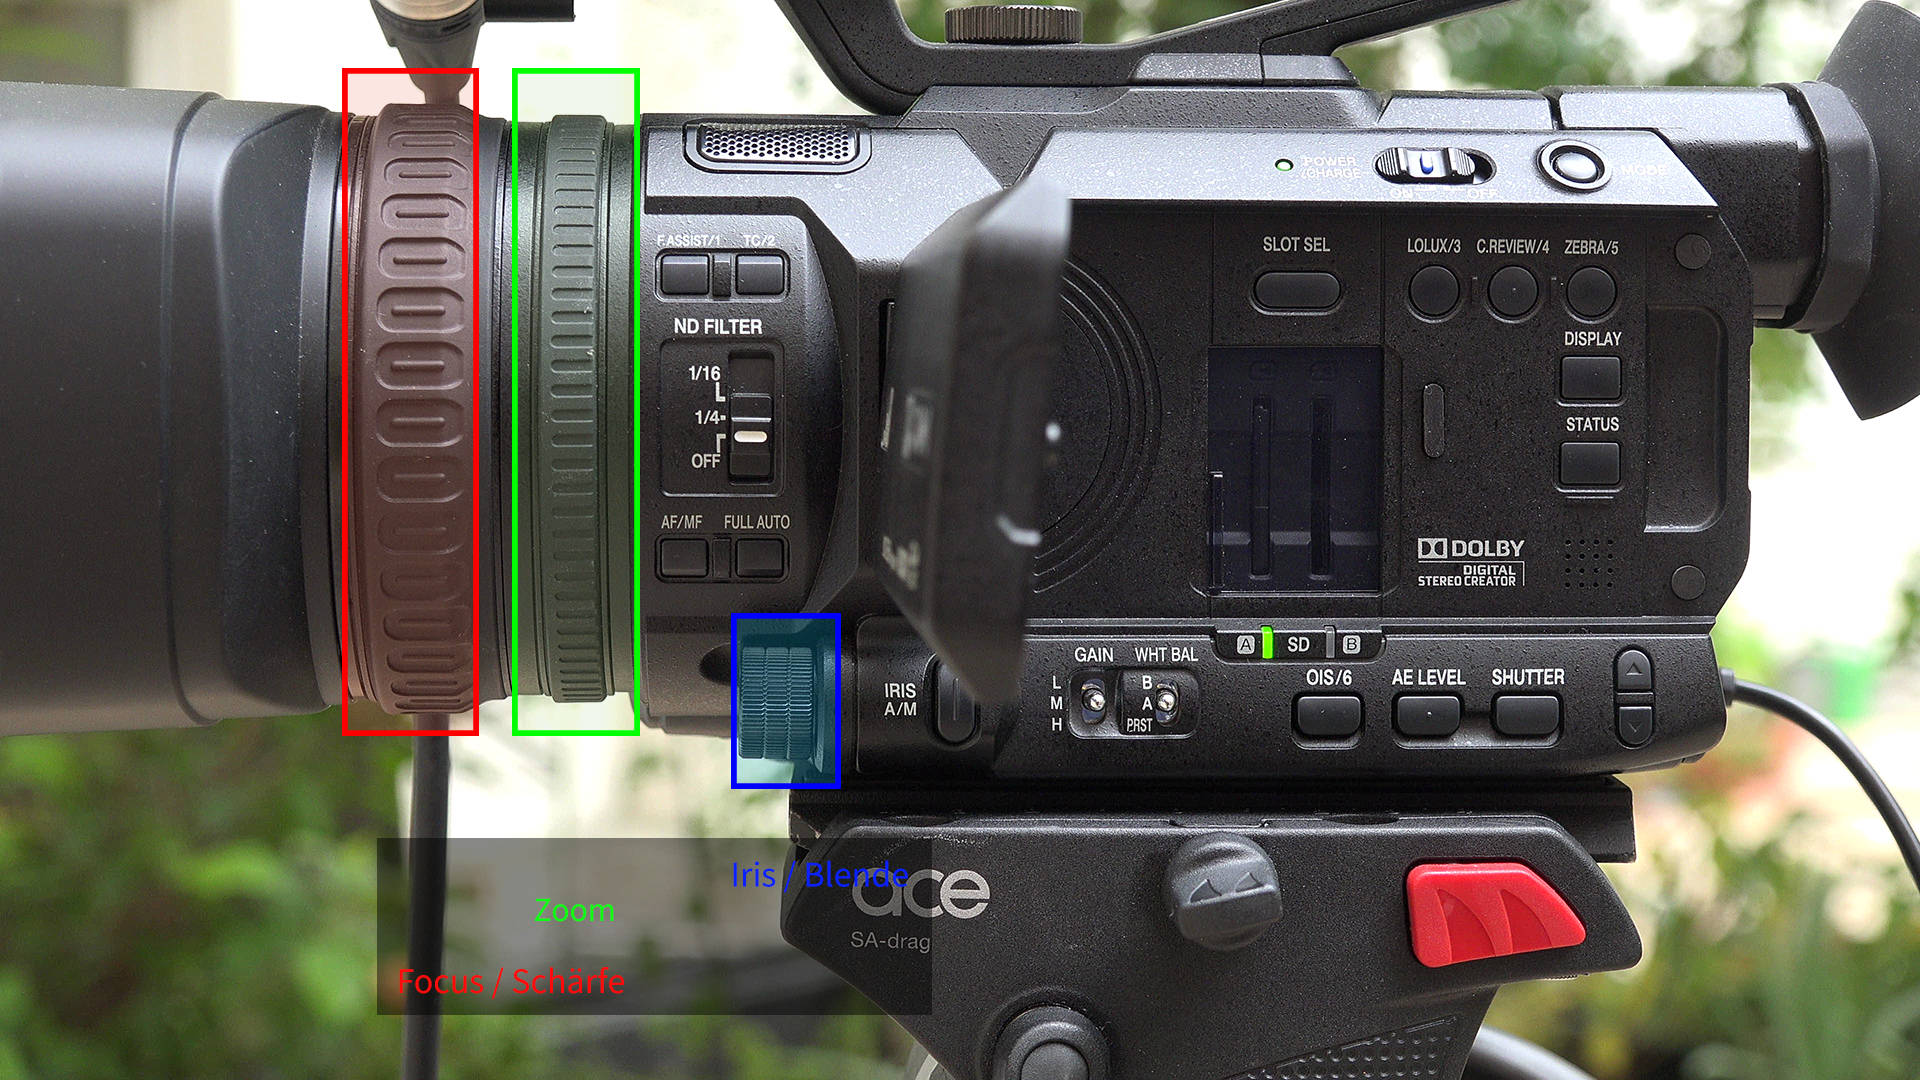
\includegraphics[width=0.9\textwidth]{images/jvc-side-annotated.jpg}
		\caption{JVC Cam}
	\end{figure}
		\column{0.5\textwidth}
		Cameras are in manual mode because of difficult lighting situation.
		\begin{description}
			\item[Left Ring/red] Focus - control sharpness of the image.
			\item[Middle Ring/green] Zoom - vary the focal length.
			\item[Right Ring/blue] Iris - will have to be adjusted throughout the day. For lighting issues talk to the A/V tech via intercom.
		\end{description}
	\end{columns}
\end{frame}

\begin{frame}{Zoom Control JVC}
	\begin{columns}[T,onlytextwidth]
		\column{0.5\textwidth}
	\begin{figure}
		\centering
		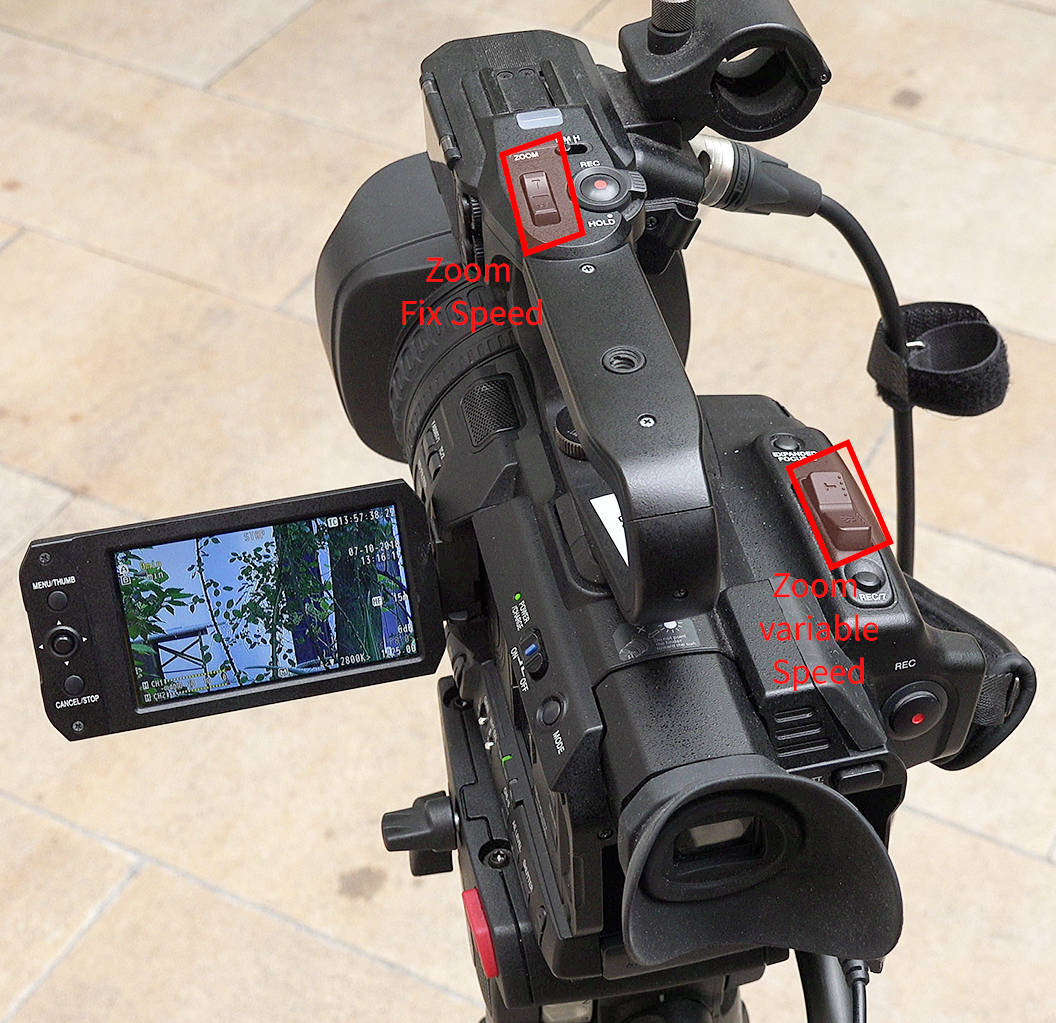
\includegraphics[width=0.9\textwidth]{images/jvc-zoom-annotated.jpg}
		\caption{JVC Cam}
	\end{figure}
		\column{0.5\textwidth}
		\begin{itemize}
			\item For smooth zoom use the zoom buttons.
			\item Gentle touch $\Rightarrow$ slow zoom
			\item Top Buttons fixed speed
		\end{itemize}
	\end{columns}
\end{frame}

\begin{frame}{Display Indicators JVC}
	\begin{columns}[T,onlytextwidth]
		\column{0.5\textwidth}
	\begin{figure}
		\centering
		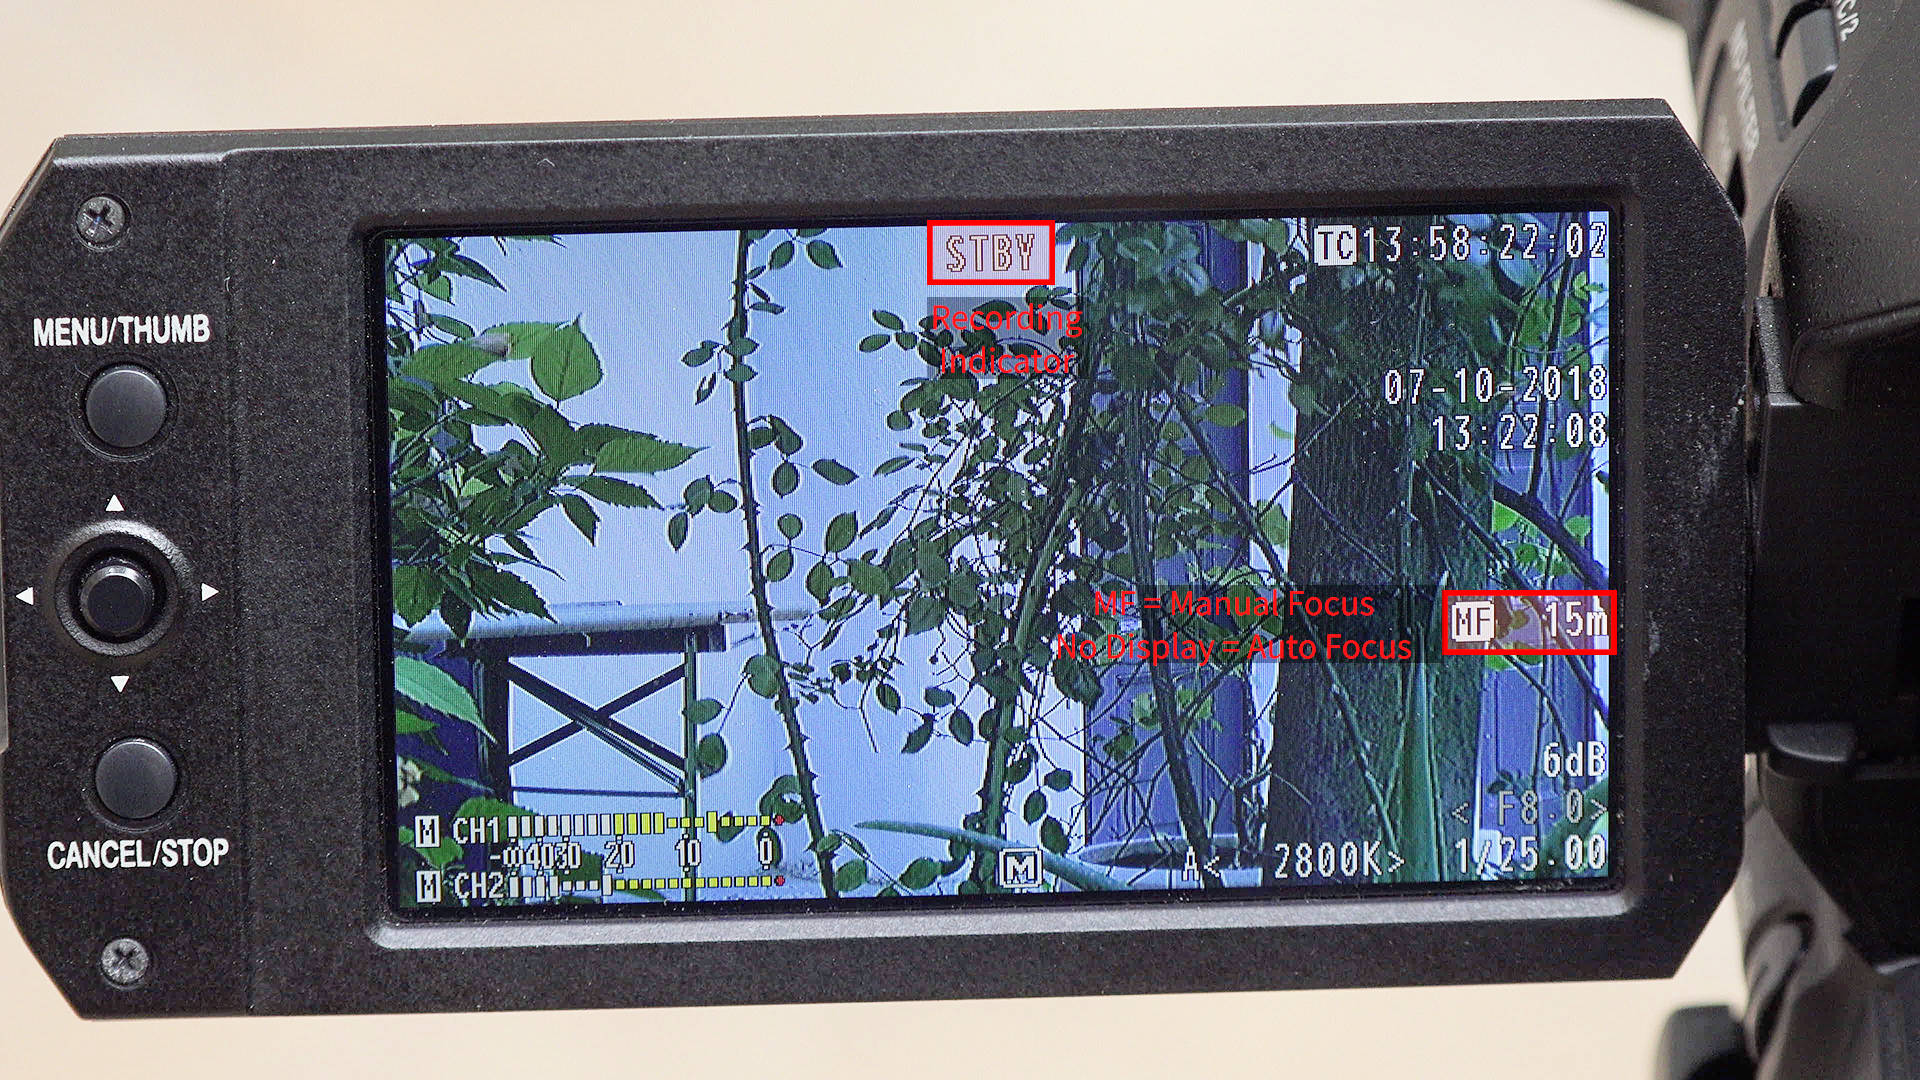
\includegraphics[width=0.9\textwidth]{images/jvc-display-annotated.jpg}
		\caption{Panasonic Display Indicators}
	\end{figure}
		\column{0.5\textwidth}
		\begin{description}
			\item[Rec Indicator] The recording must always run, even during the break.
			\item[Focal Indicator] Use only manual focus!
		\end{description}
		\metroset{block=fill}
		\begin{alertblock}{Alert}
			Alert the A/V-Technician if something's wrong.
		\end{alertblock}
	\end{columns}
\end{frame}

% !TEX root = ../main.tex

%\begin{frame}{Tripod Handle Controls}
%	\begin{columns}[T,onlytextwidth]
%	\column{0.5\textwidth}
%	\begin{figure} 
%		\centering
%		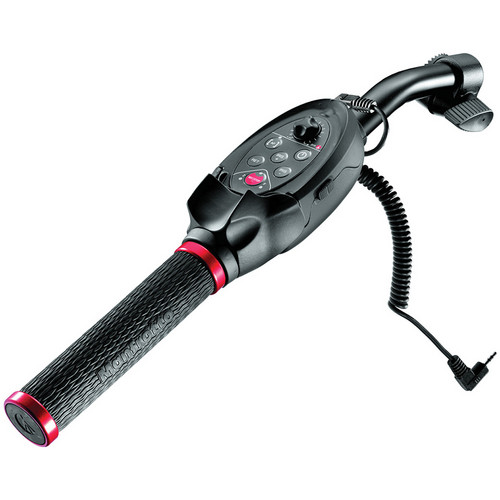
\includegraphics[width=0.7\textwidth]{images/tripod-handle.jpeg}
%		\caption{Tripod Handle}
%	\end{figure}
%
%	\column{0.5\textwidth}
%	Beware: various models in use.
%	\begin{description}
%		\item[Zoom Control] lever above red ring
%		\item[Red Button] Start/stop recording, don't touch
%		\item[Other Buttons] markings on the handle
%   \end{description}
%	\end{columns}
%\end{frame}

\begin{frame}{Tripod}
	\begin{columns}[T,onlytextwidth]
	\column{0.4\textwidth}
	\begin{figure} 
		\centering
		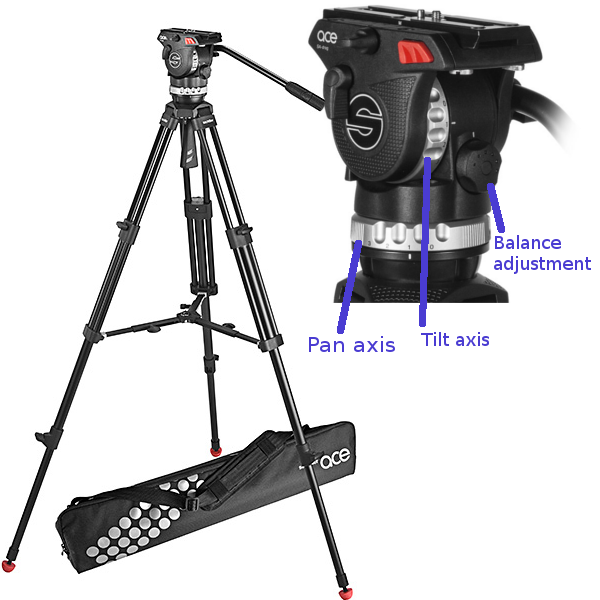
\includegraphics[width=0.9\textwidth]{images/tripod-complete.png}
		\caption{Tripod}
	\end{figure}
	
	\column{0.6\textwidth}
	\begin{itemize}
			\item Should be level - check the water bubble.
			\item Variable brakes - can be adjusted to your needs.
			\item Tilt axis should be balanced, so that the camera doesn't tilt up or down on its own.
			\item Pan axis is needed all of the time. Set it so you can do smooth pans all over the stage.
		\end{itemize}
		\metroset{block=fill}
		\begin{alertblock}{Alert}
			Alert the A/V-Technician if something's wrong or misplaced.
		\end{alertblock}
	\end{columns}
\end{frame}

\begin{frame}{SD-Card Recording}
		\begin{itemize}
			\item Two SD-Cards in every Camera
			\item Backup Recording
			\item Turn on Recording before first shift in the morning -> Red Dot somewhere in the Display.
			\item Control Recording Time remaining. 
		\end{itemize}
		\metroset{block=fill}
		\begin{alertblock}{Alert}
			Alert the A/V-Technician if something's wrong or not running.
		\end{alertblock}
\end{frame}



\section{Video Mixer Tools}
% !TEX root = ../main.tex

\begin{frame}{Voctomix2 - Overview}
	\begin{figure}
		\centering
		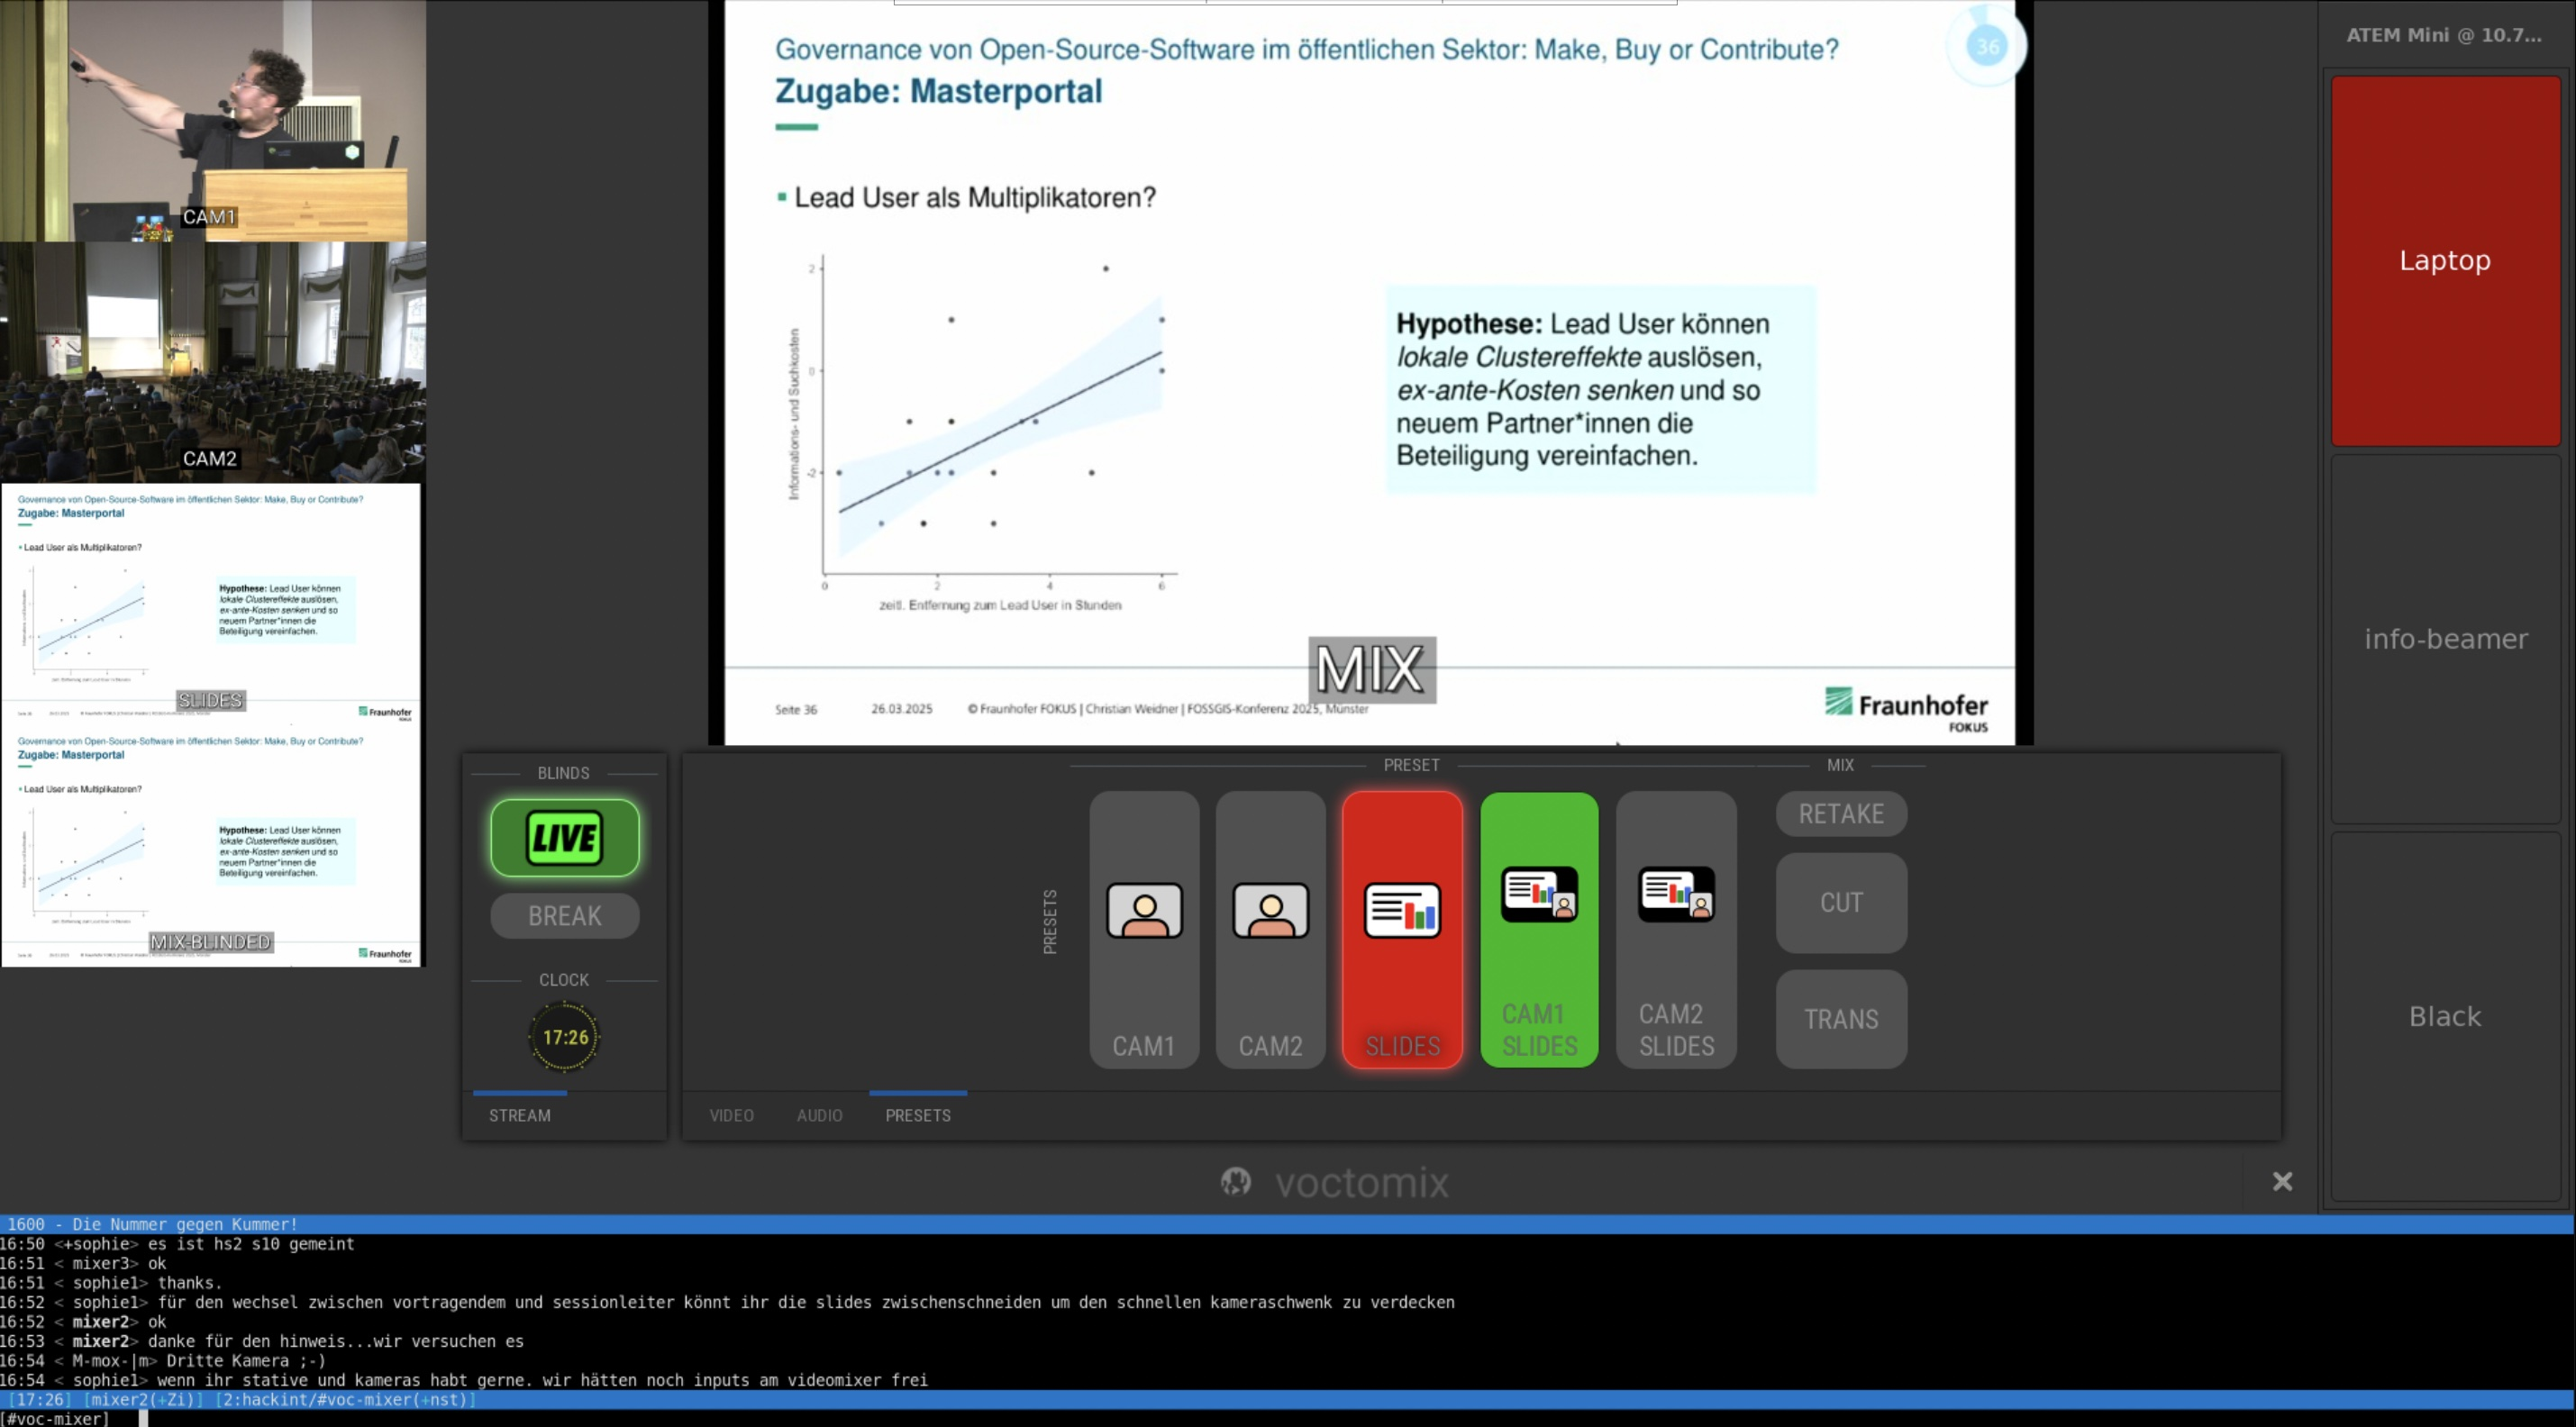
\includegraphics[width=.8\textwidth]{images/voctomix2-overview.jpg}
		% To say: Voctomix in the middle, py-atem-gtk, mix live/pause, IRC
		\caption{Voctomix2 - Overview (presets)}
	\end{figure}
\end{frame}

\section{Mixing with Presets}
\begin{frame}{Voctomix2 - Presets}
	\begin{figure}
		\centering
		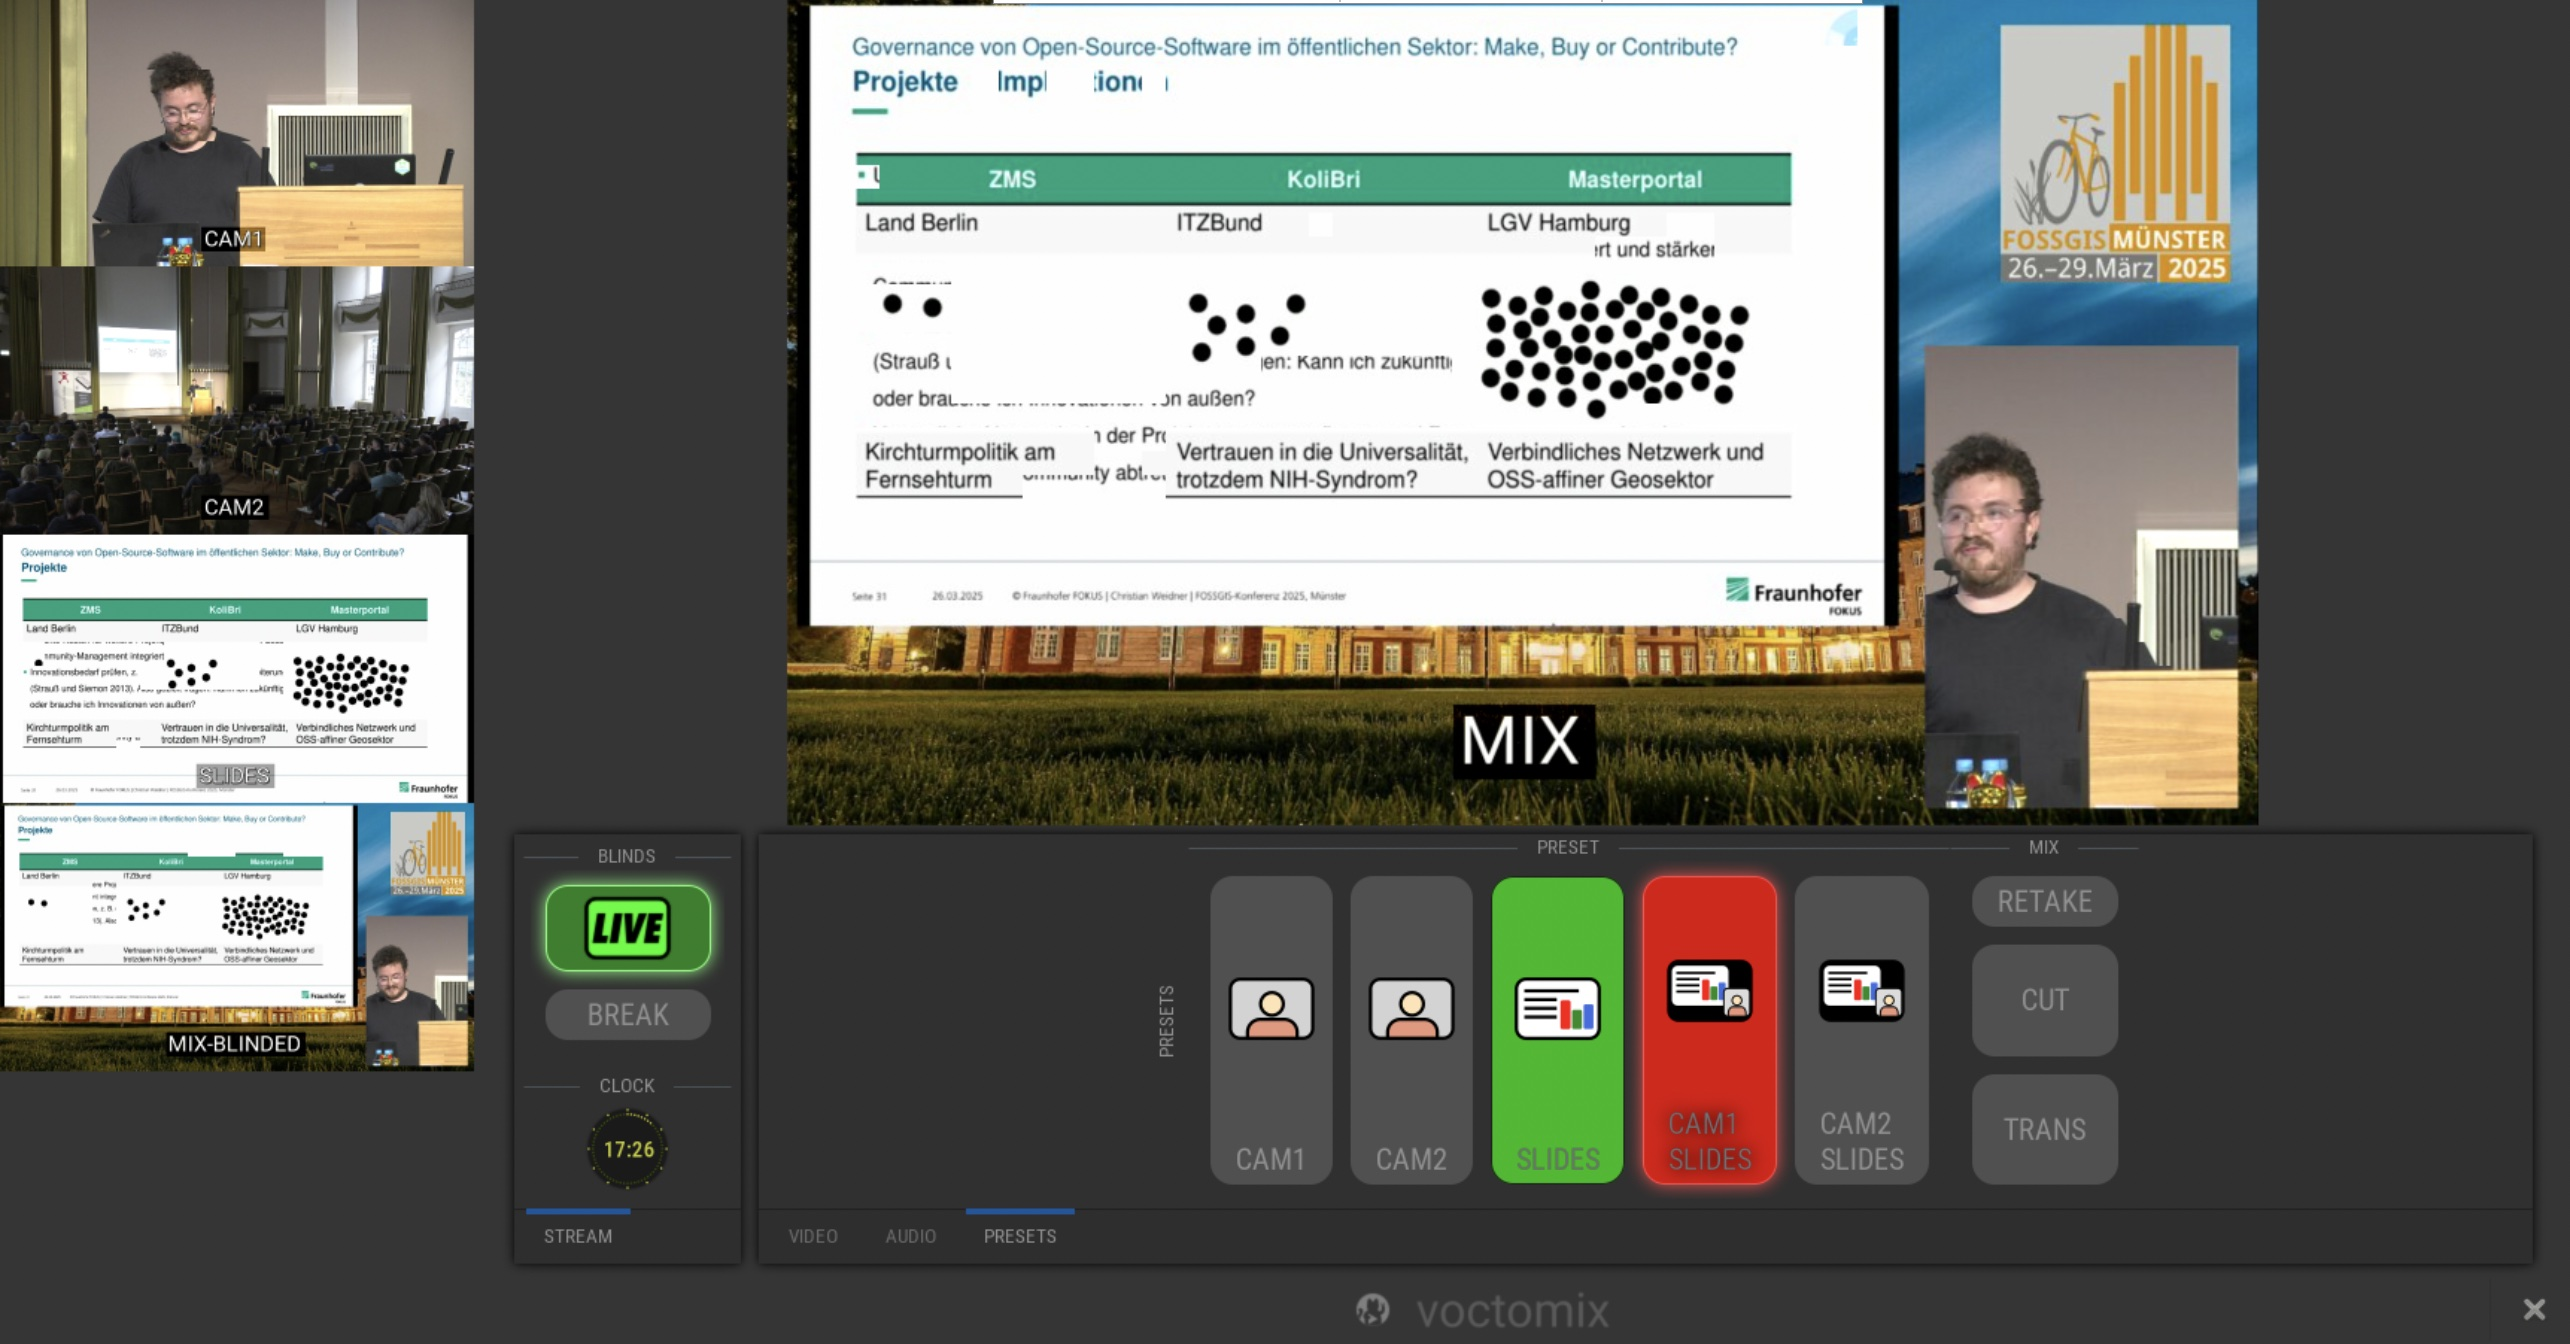
\includegraphics[width=0.9\textwidth]{images/voctomix2-presets-lecture.jpg}
		\caption{Voctomix2 Presets: Lecture Mode}
	\end{figure}
\end{frame}

\begin{frame}{Voctomix2 - Presets}
	\begin{figure}
		\centering
		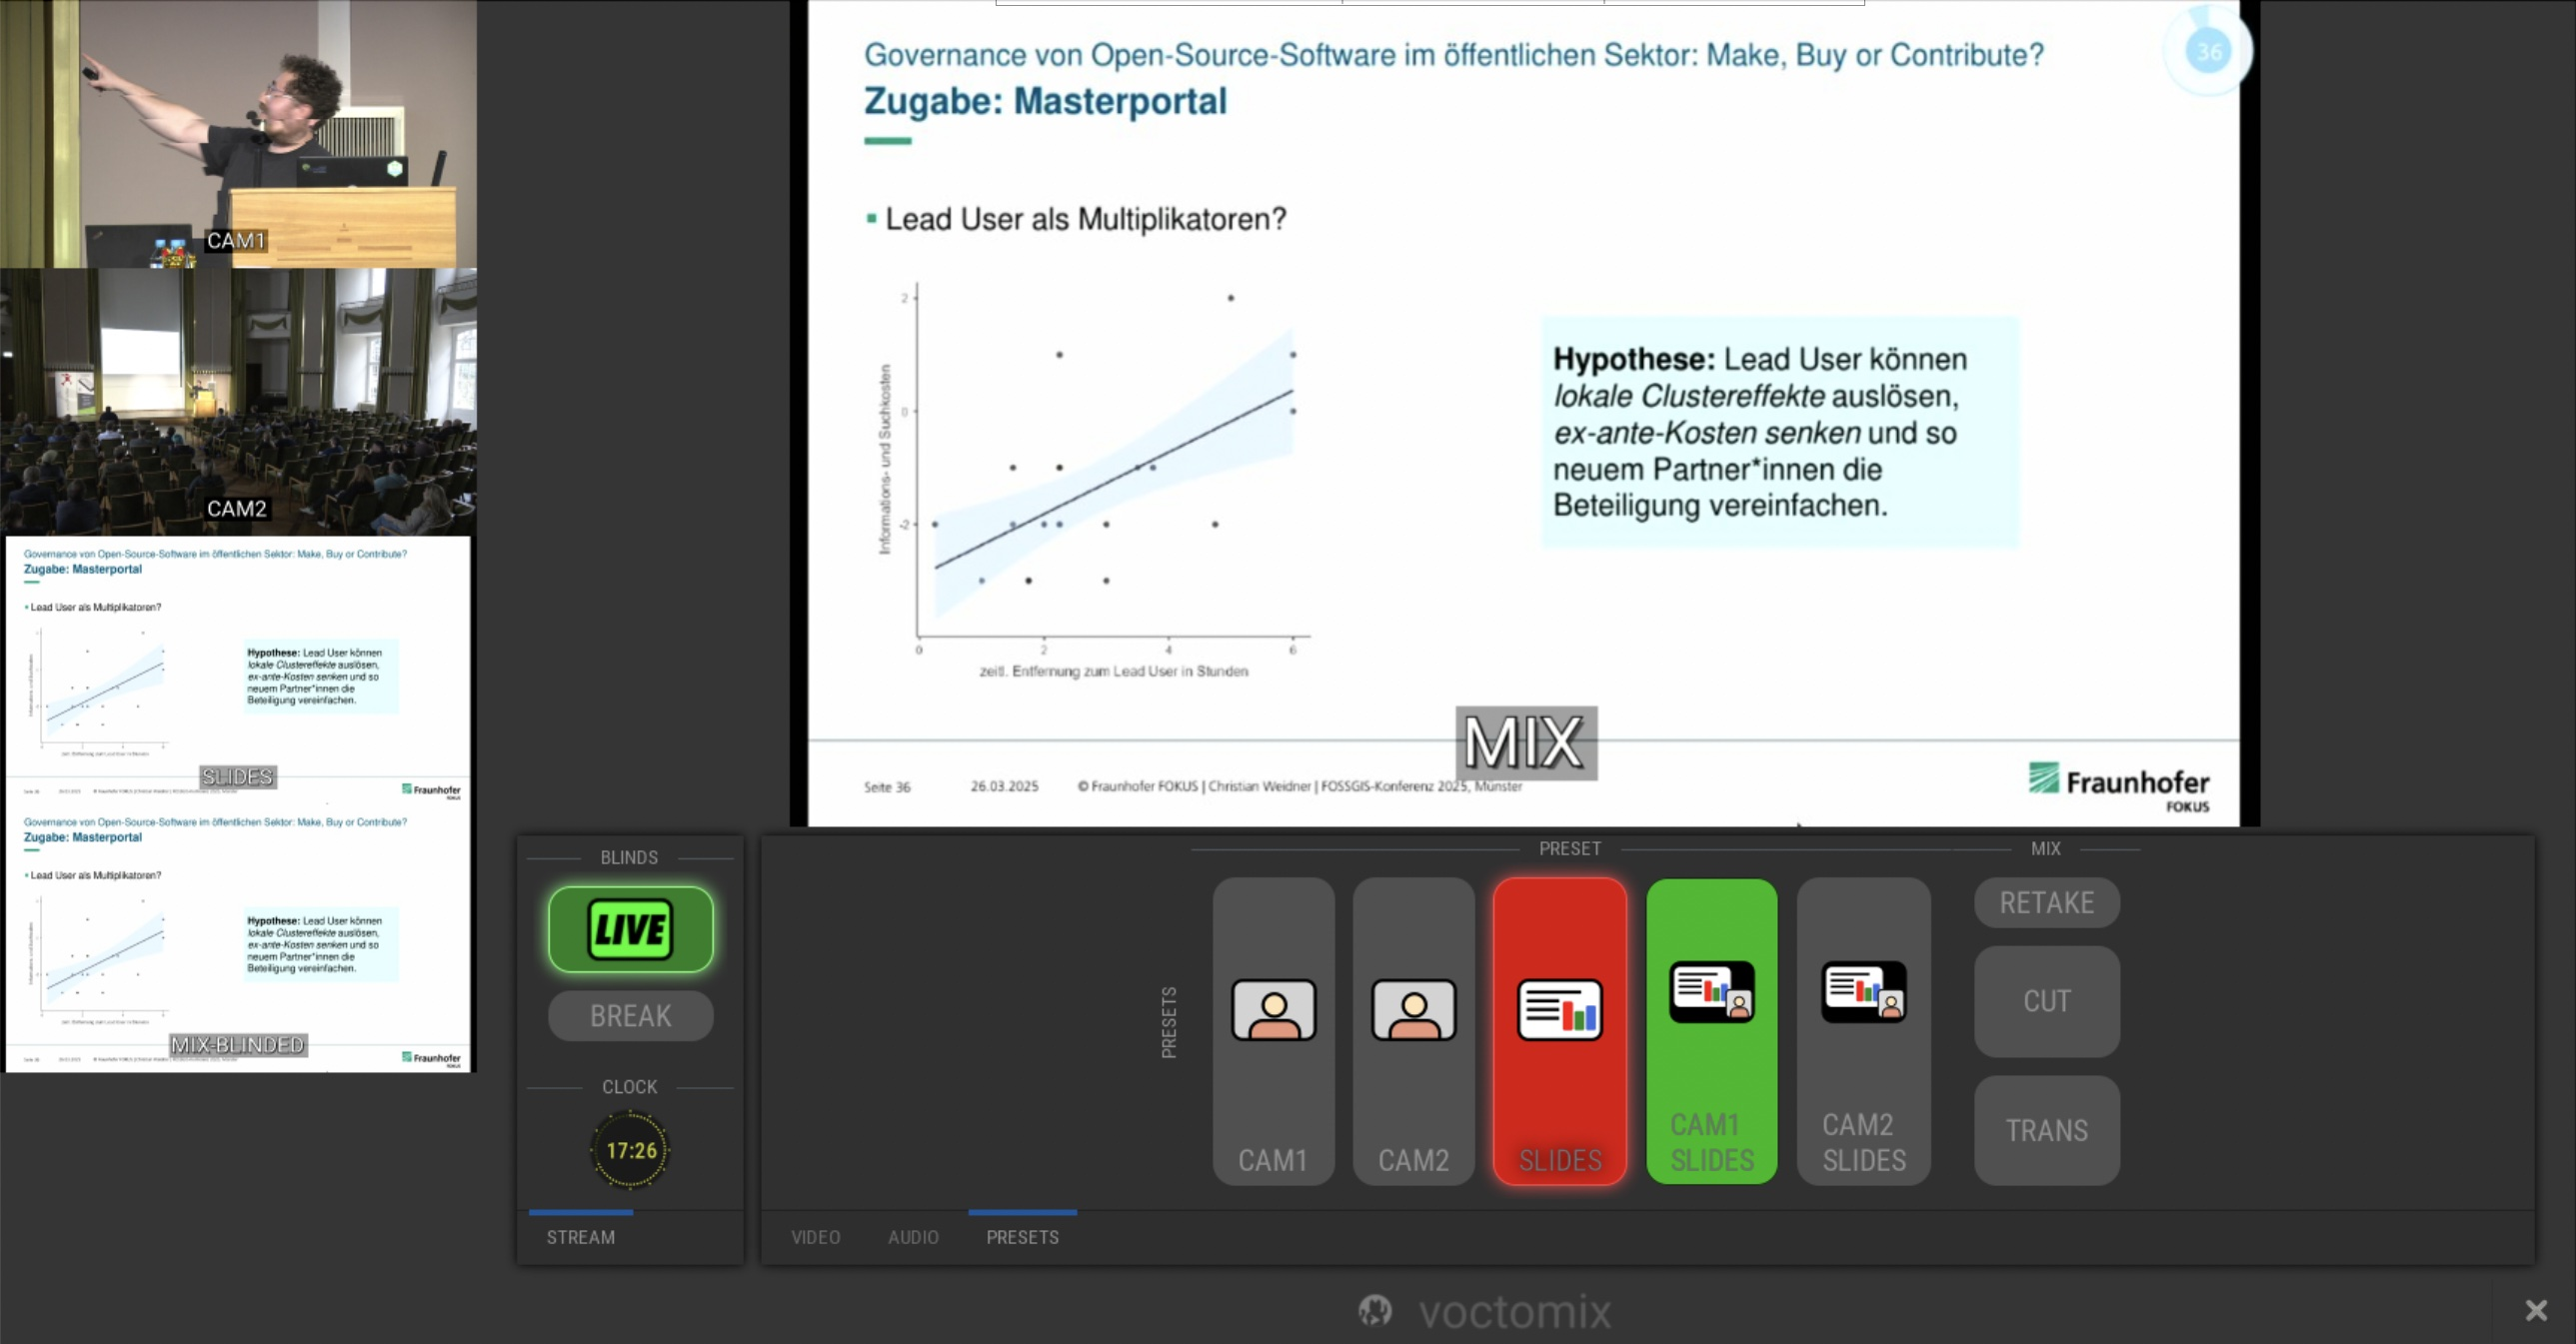
\includegraphics[width=0.9\textwidth]{images/voctomix2-presets-slides.jpg}
		\caption{Voctomix2 Presets: Slides Fullscreen}
	\end{figure}
\end{frame}

\section{Classical Mode}
\begin{frame}{Voctomix2 - Pre-Select}
	\begin{figure}
		\centering
		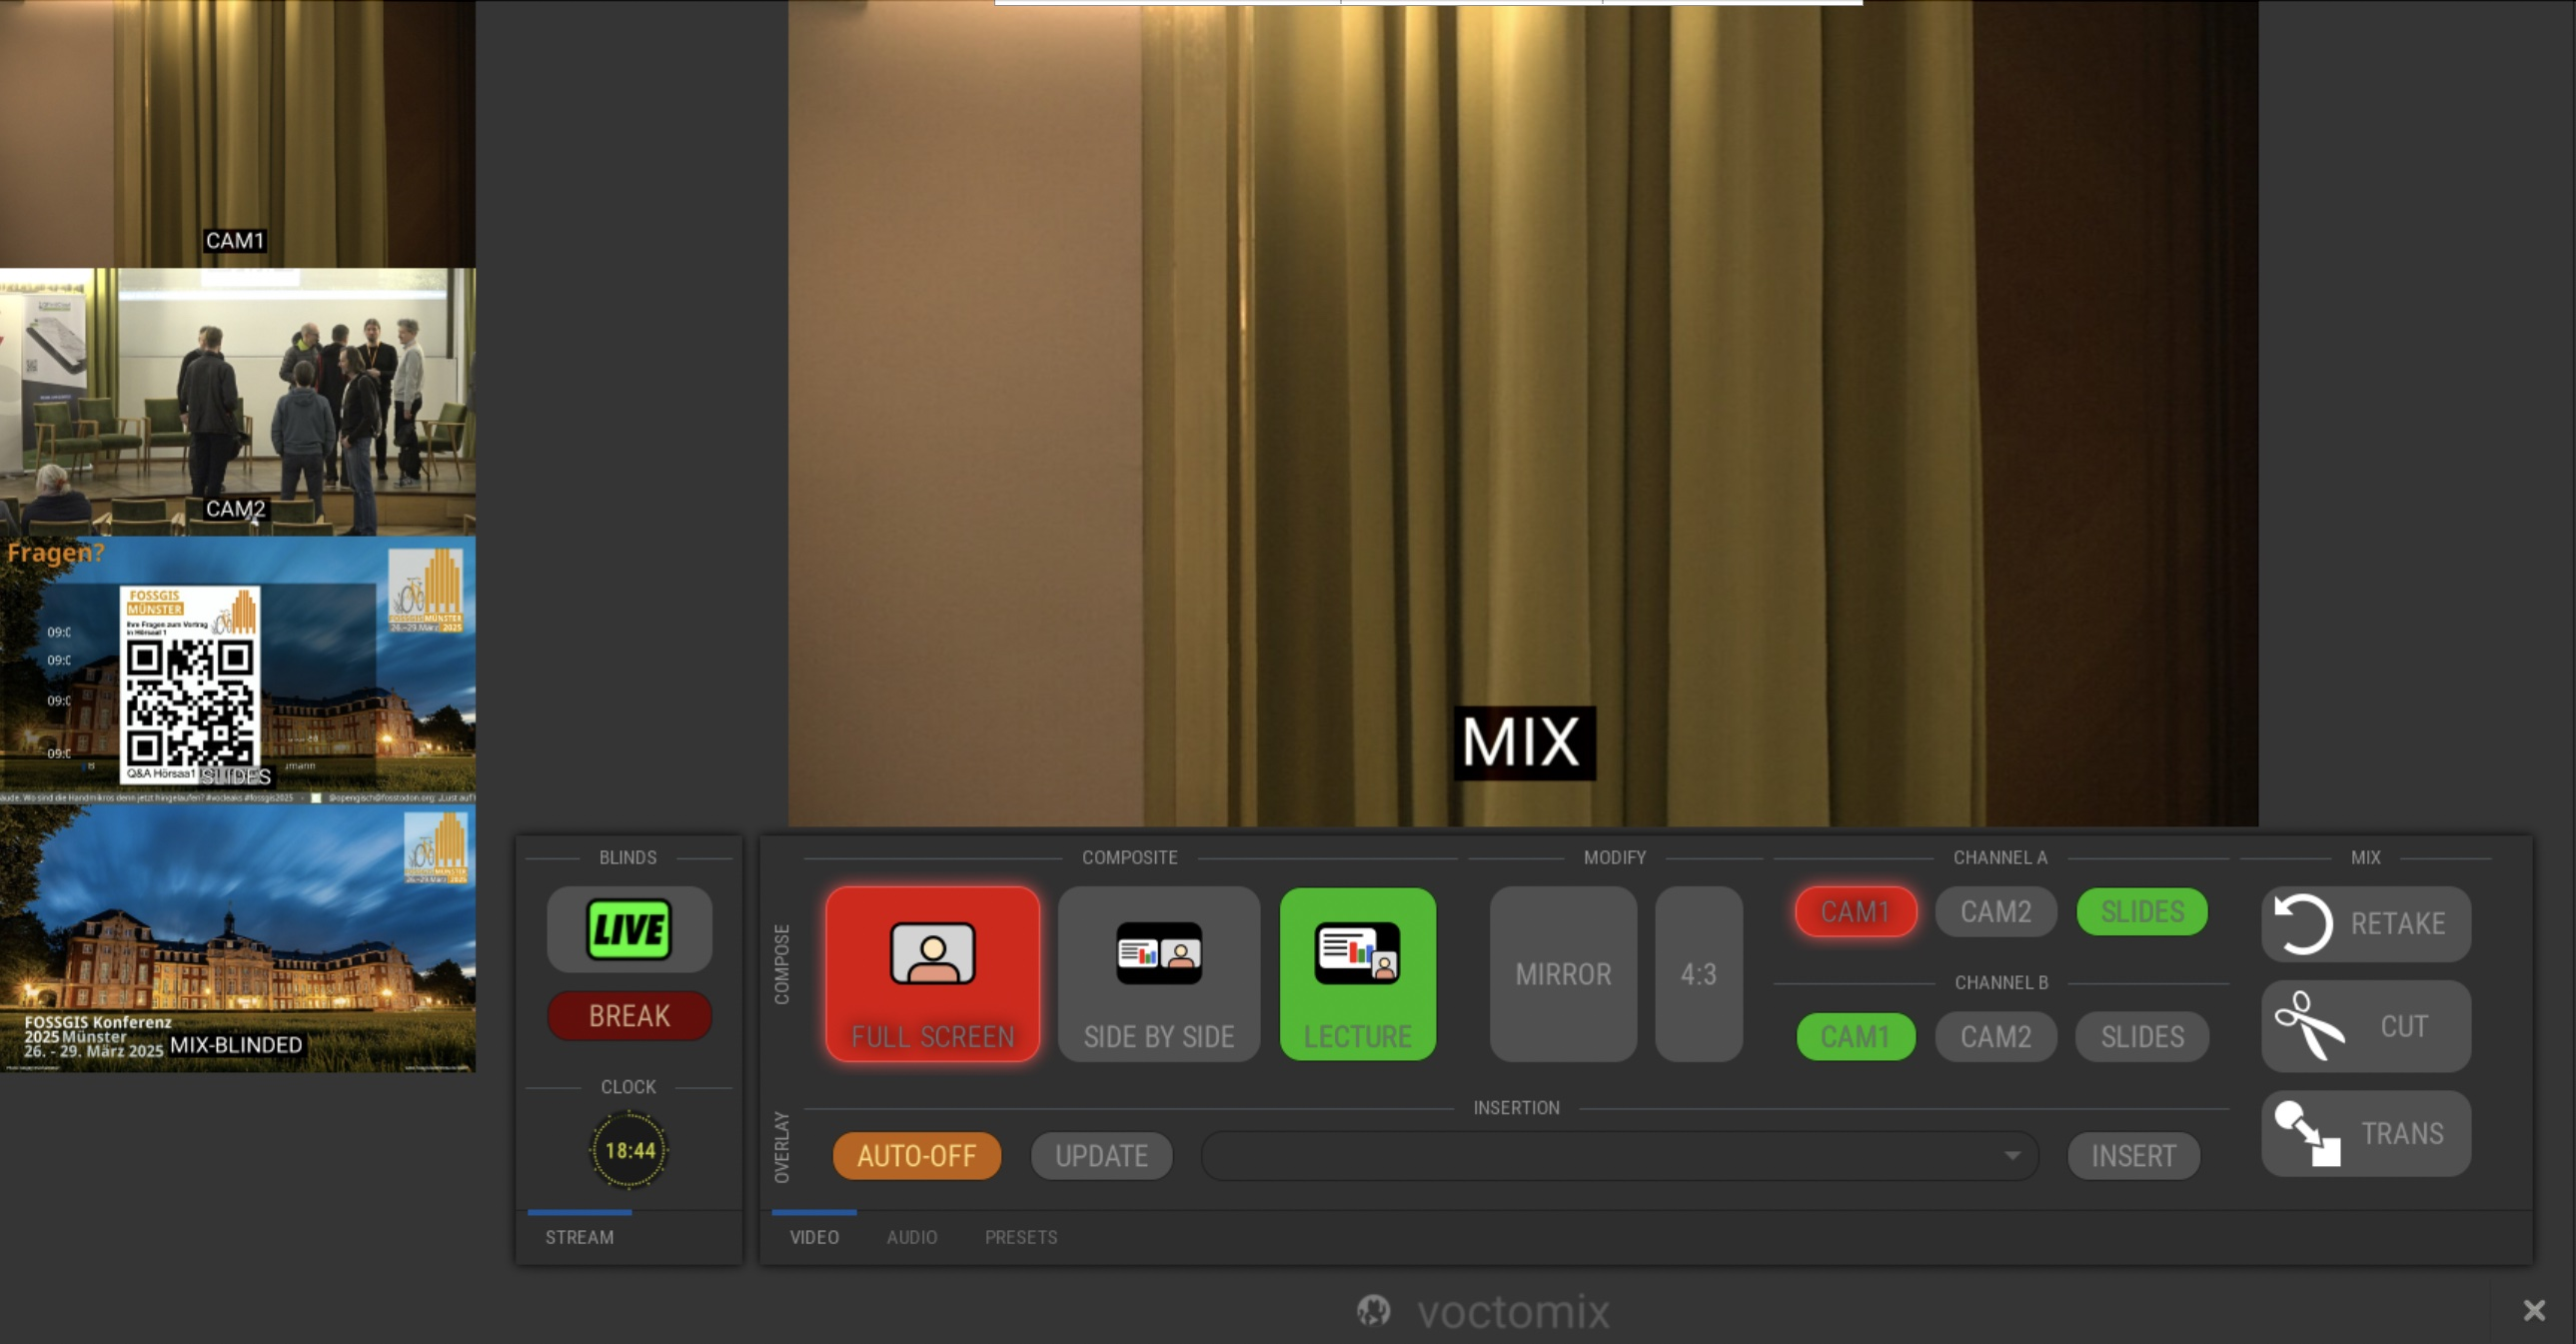
\includegraphics[width=.9\textwidth]{images/voctomix2-lecture_select.jpg}
		% To say: Next scene is shown with solid color, current scene with border, switch with trans or cut button
		\caption{Voctomix2 - Lecture Mode - Pre-Selected}
	\end{figure}
\end{frame}

\begin{frame}{Voctomix2 - Lecture Mode}
	\begin{figure}
		\centering
		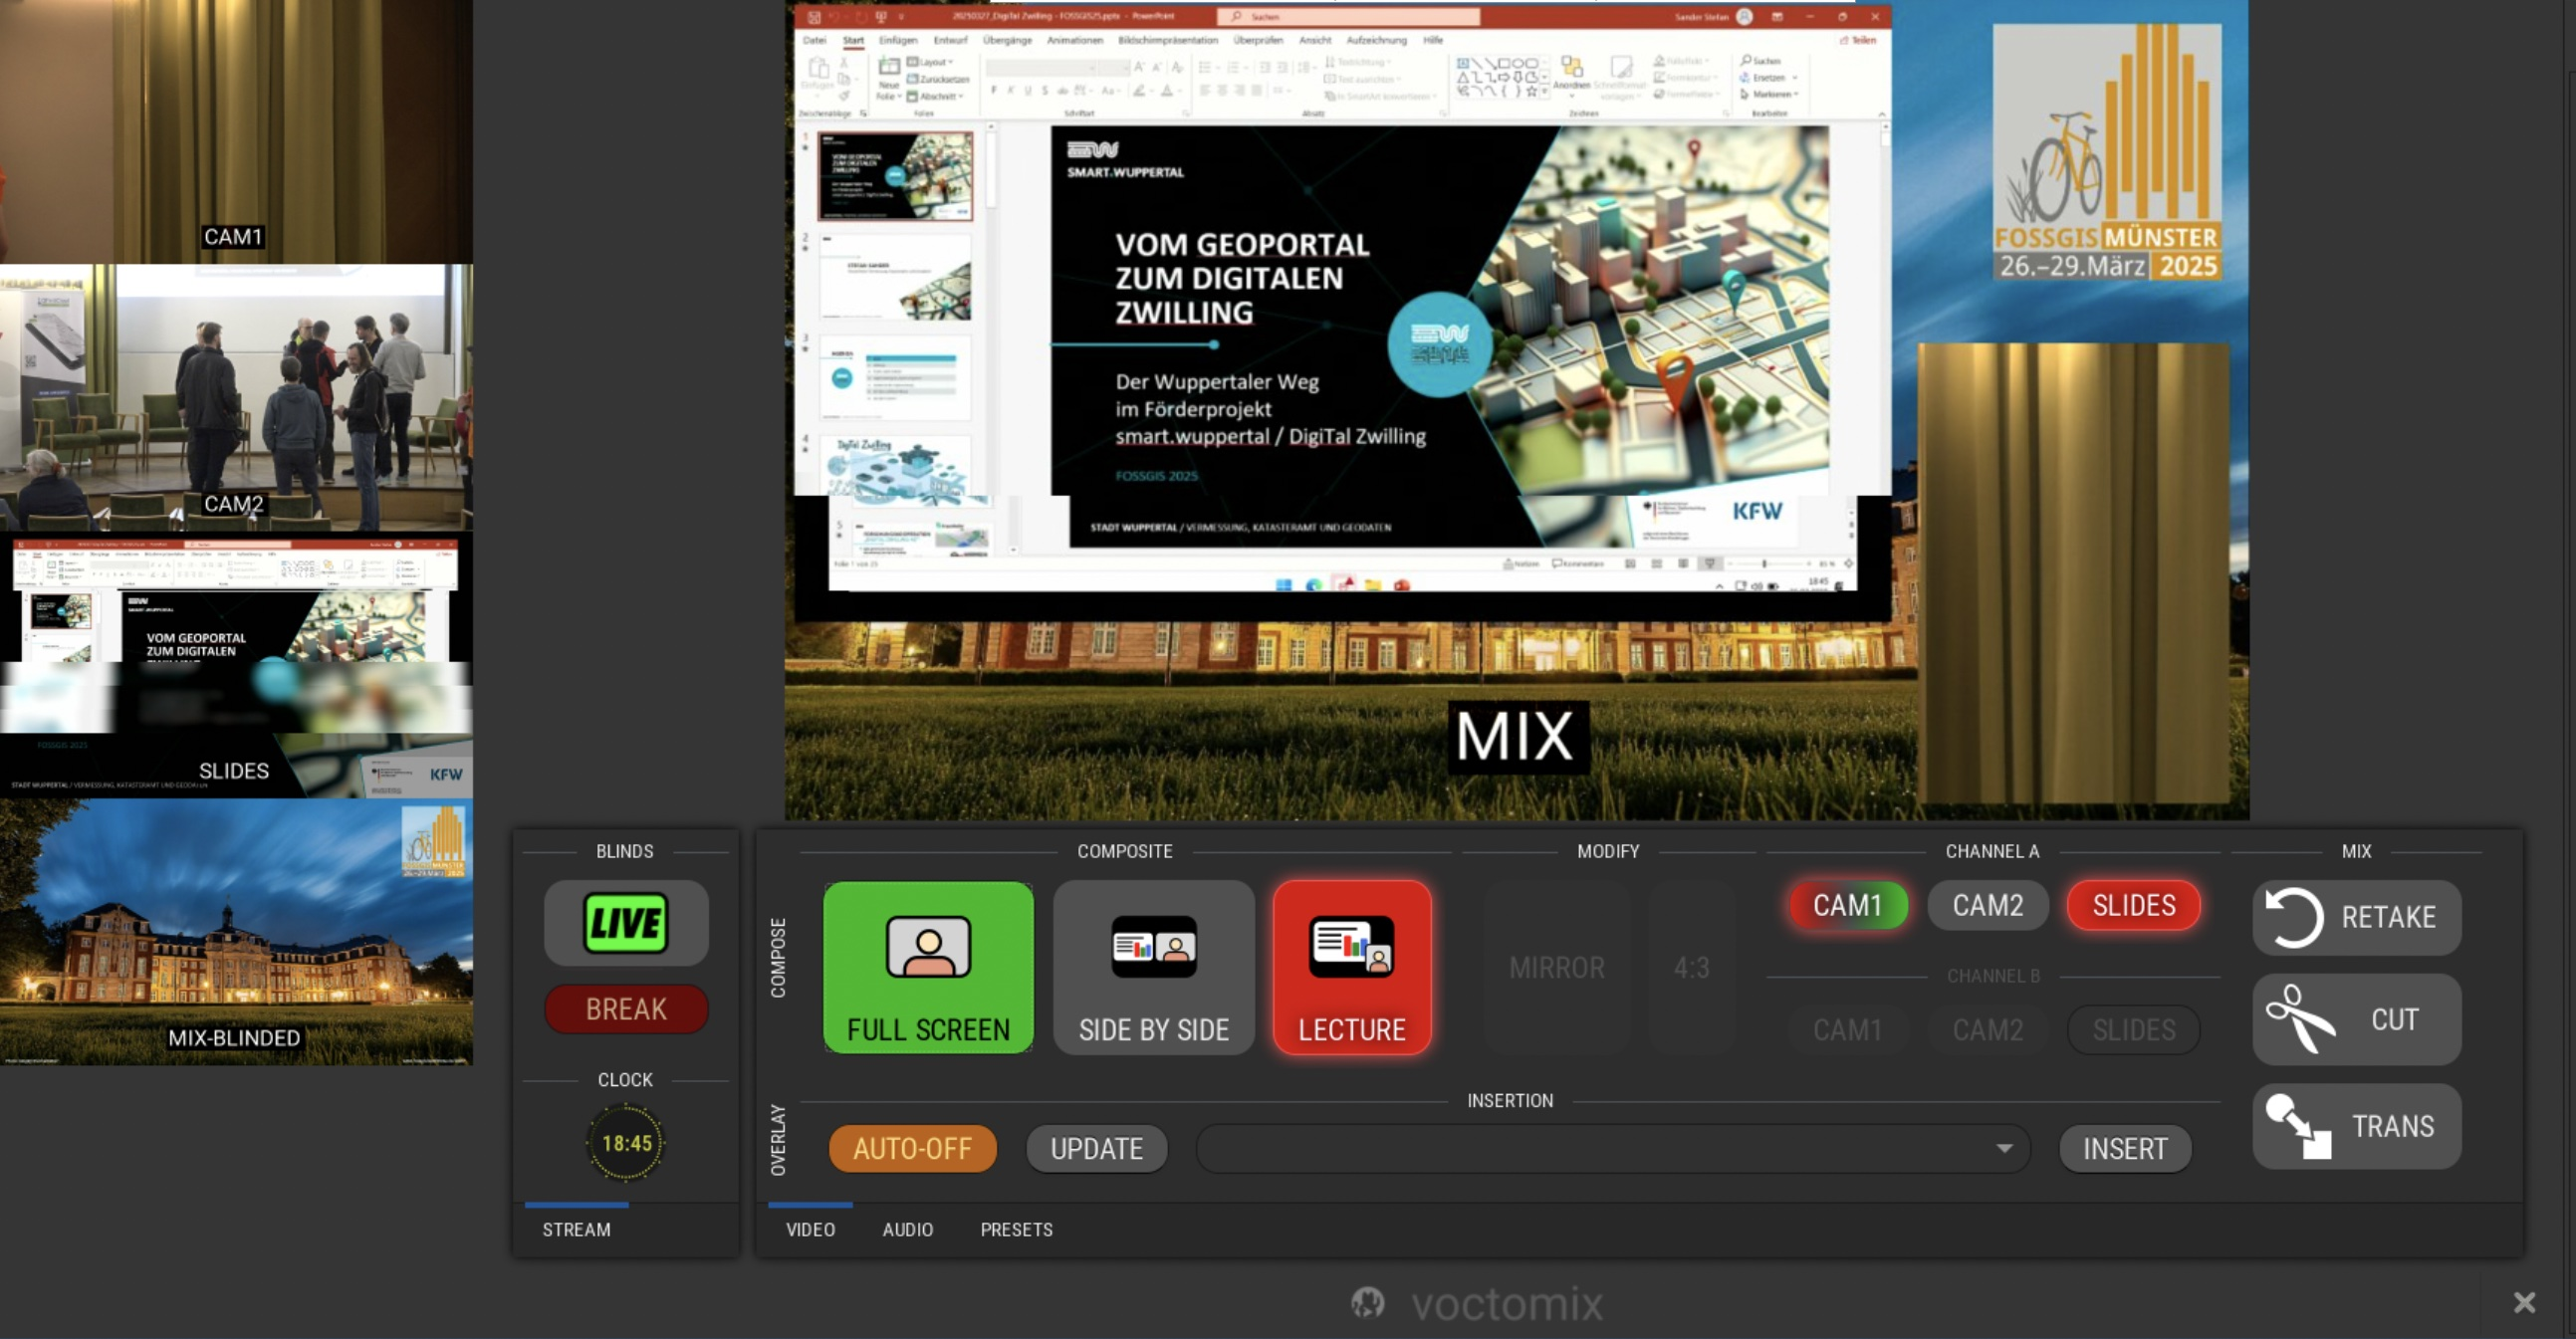
\includegraphics[width=.9\textwidth]{images/voctomix2-lecture.jpg}
		% To say: Pre-select and live mix switch places
		\caption{Voctomix2 - Lecture Mode - Live}
	\end{figure}
\end{frame}

\begin{frame}{Voctomix2 - Lecture Mode 4:3}
	\begin{figure}
		\centering
		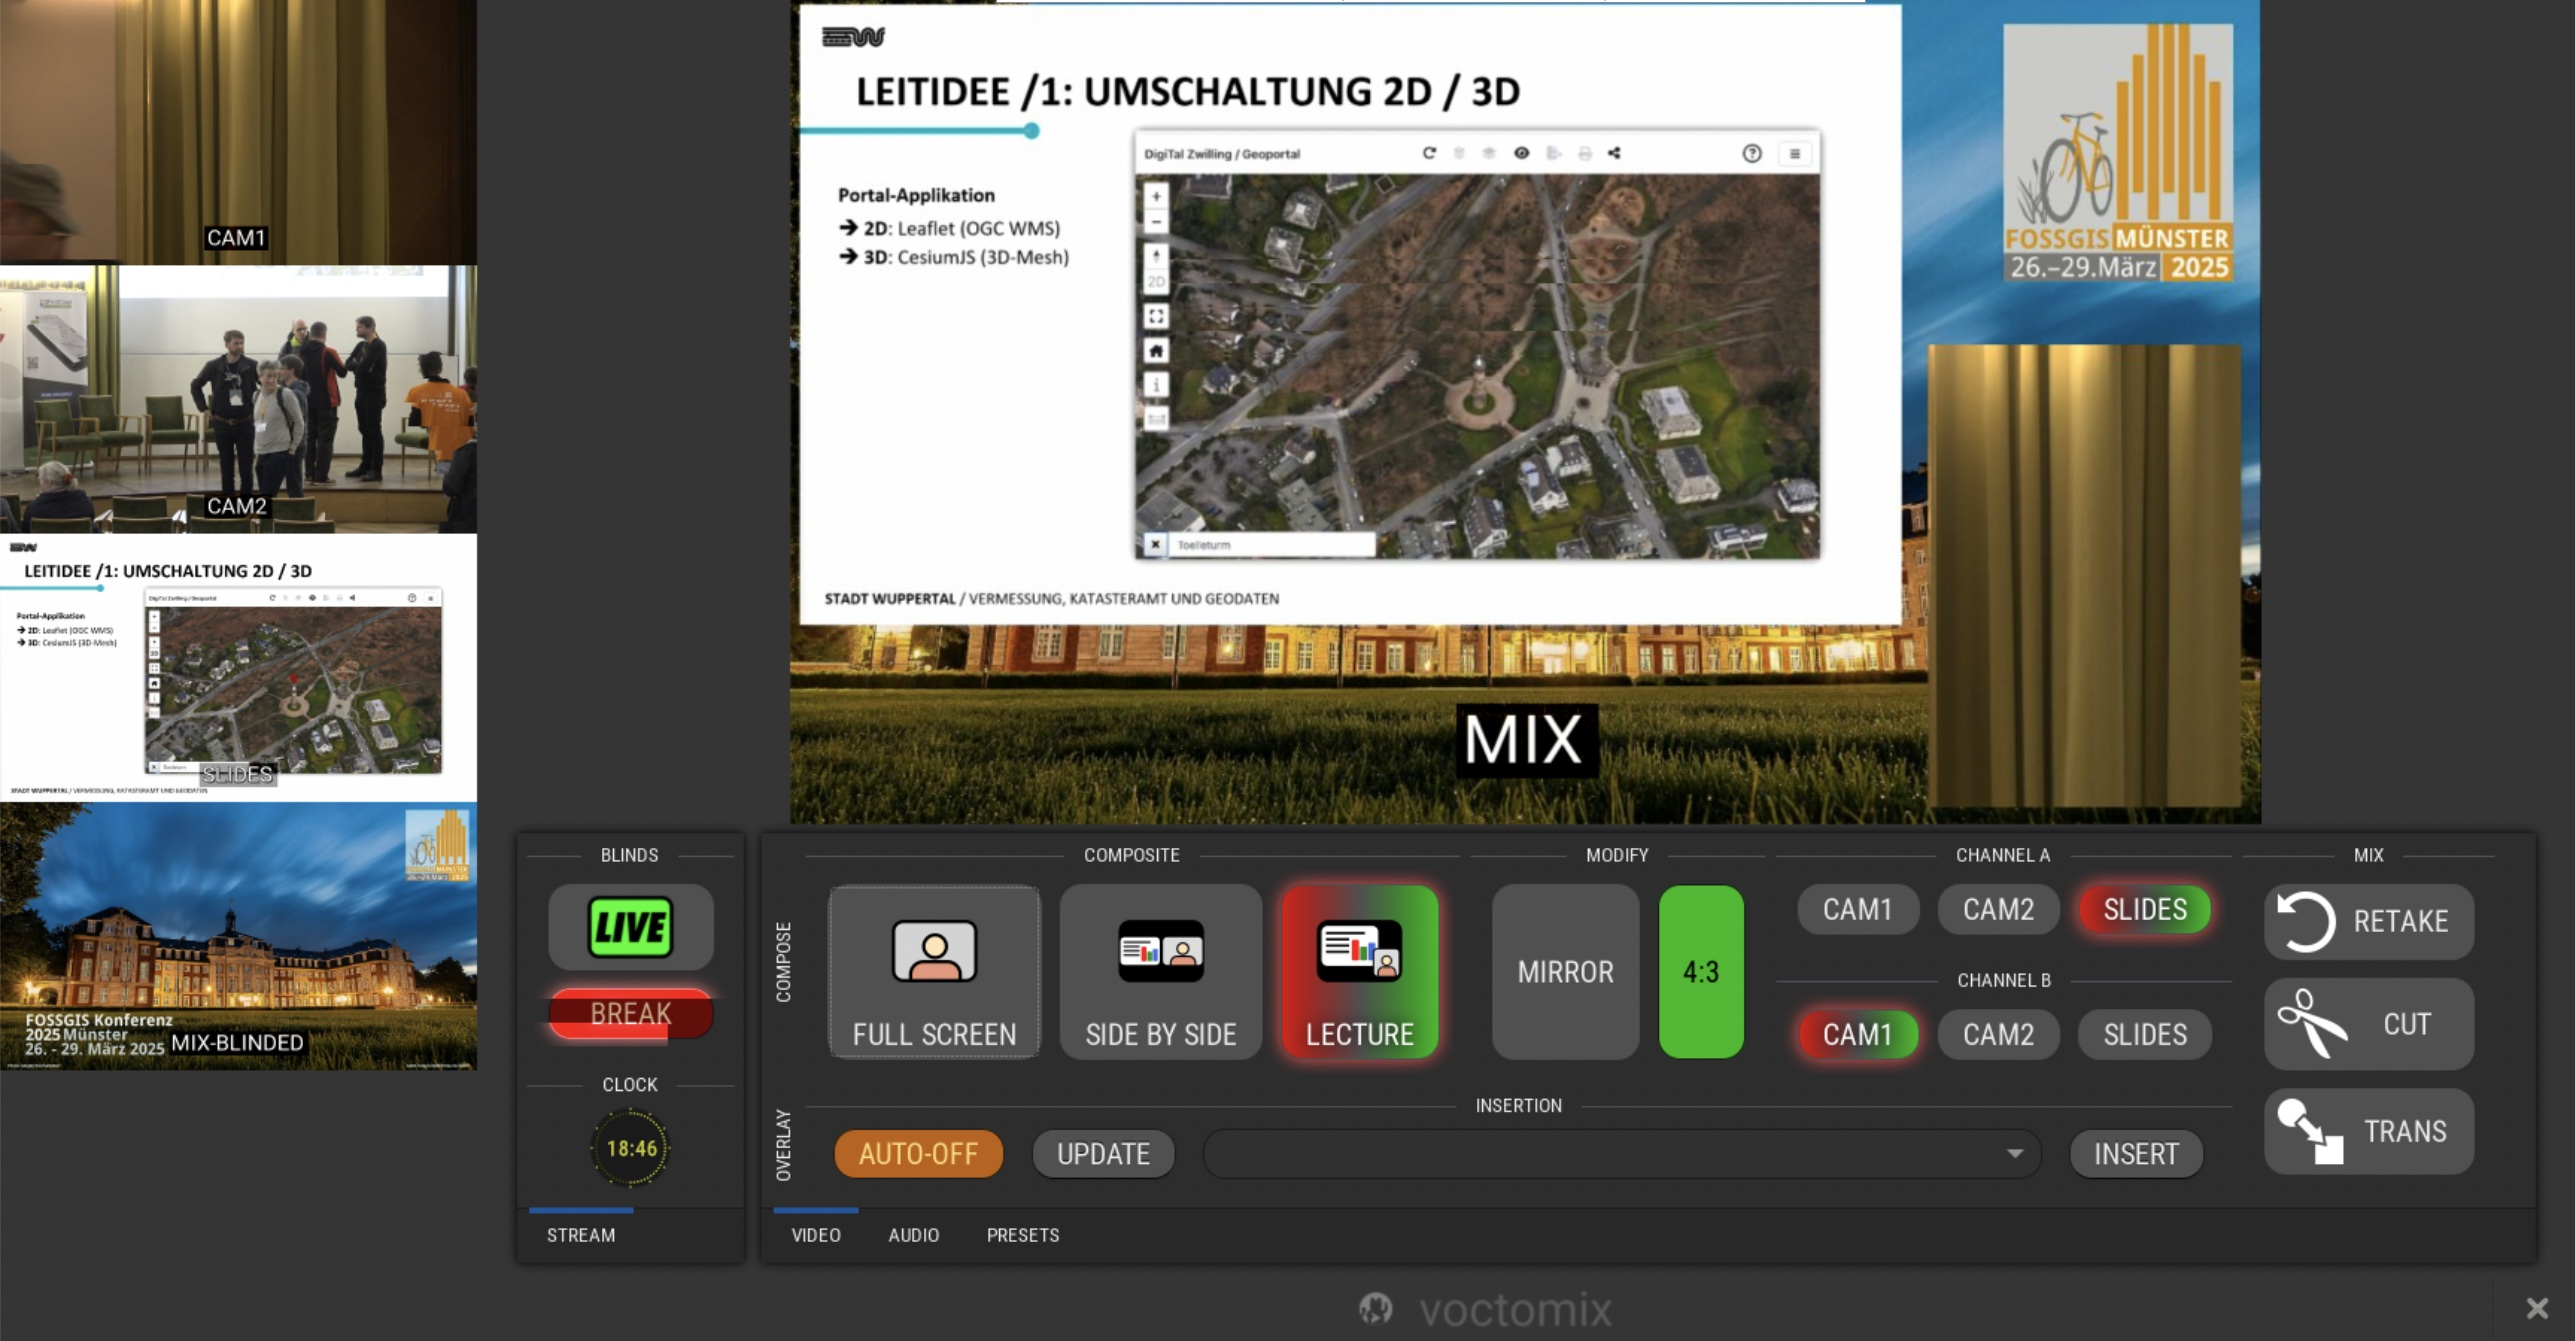
\includegraphics[width=.9\textwidth]{images/voctomix2-lecture_43_select.jpg}
		% To say: Select 4:3 mode
		\caption{Voctomix2 - Lecture Mode 4:3 - Pre-Selected}
	\end{figure}
\end{frame}

\begin{frame}{Voctomix2 - Lecture Mode 4:3}
	\begin{figure}
		\centering
		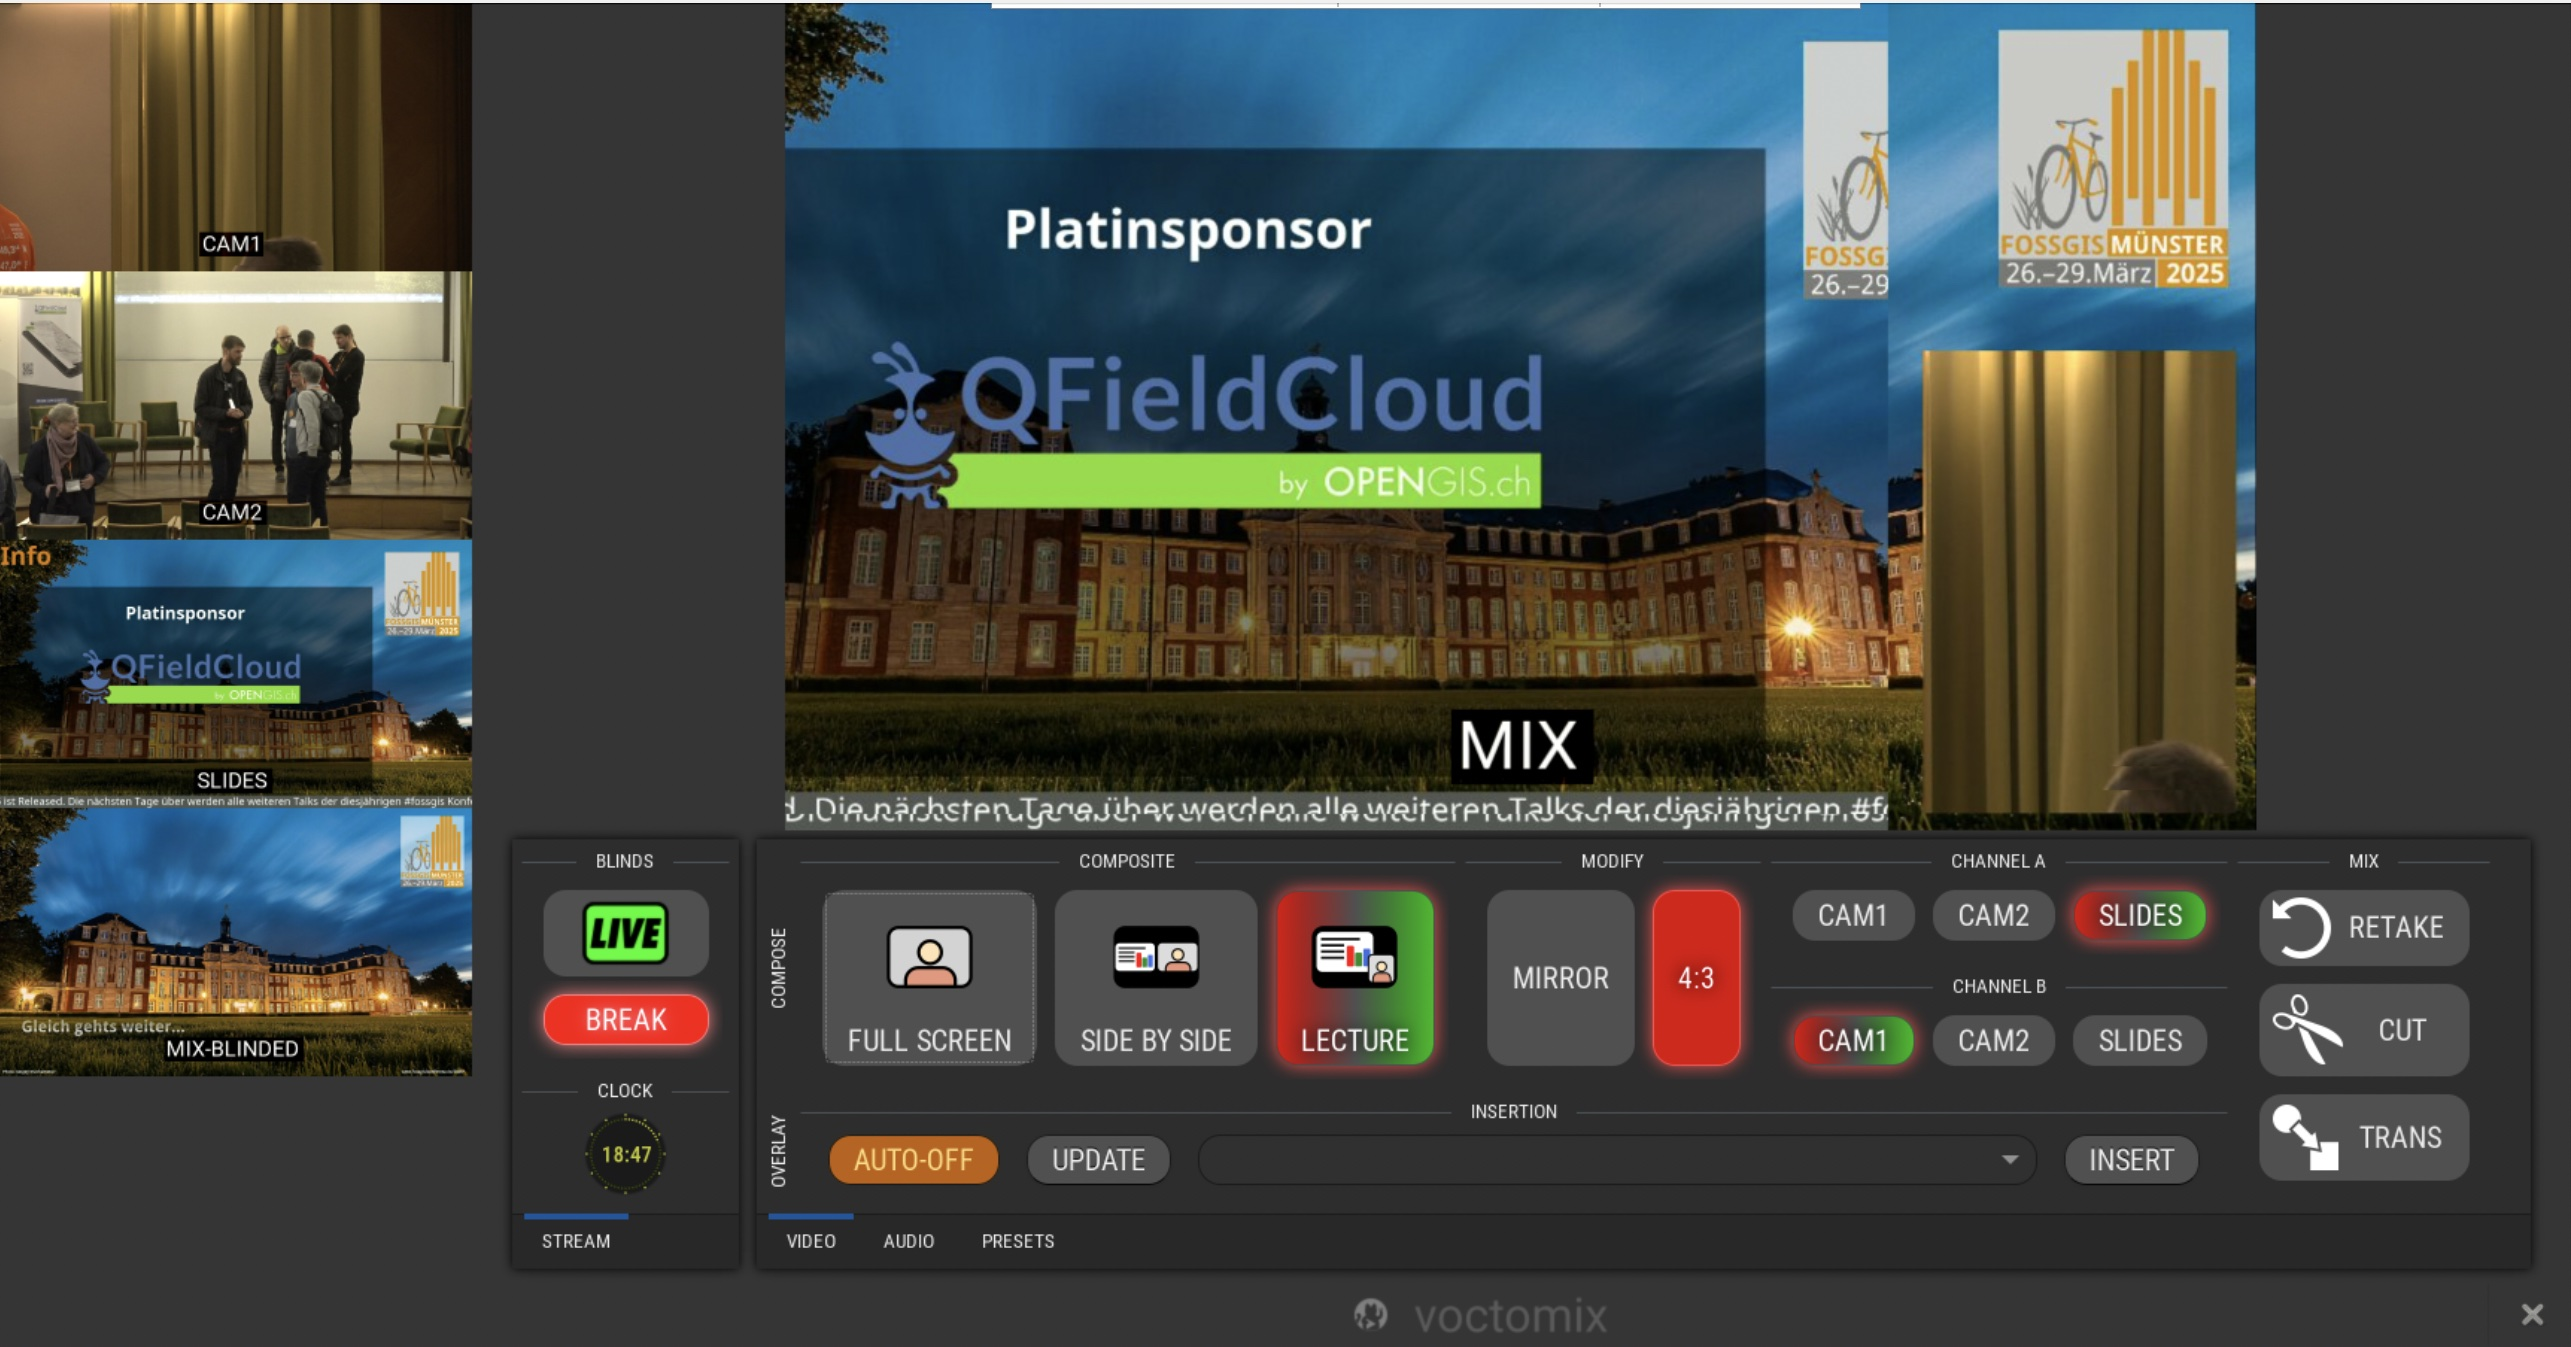
\includegraphics[width=.9\textwidth]{images/voctomix2-lecture_43.jpg}
		% To say: That's how 4:3 looks
		\caption{Voctomix2 - Lecture Mode 4:3 - Live}
	\end{figure}
\end{frame}

\section{Video Mixing Guidelines}
\begin{frame}{Mixing Guidelines - Hard Rules}
	\begin{itemize}
		\item \textbf{All} you are doing is \textbf{recorded} and will be published.
		\item The Audience is \textbf{not to be filmed}. Cut away if faces of people not on the stage appear.
		\item \textbf{Slides are important}
		\item Slides stay on till the text has been read \textbf{twice}.
		\item Show new slides \textbf{immediately}.
	\end{itemize}
\end{frame}

\begin{frame}{Mixing Guidelines - Softer Hints}
	\begin{itemize}
		\item Start early – opening announcements of the Herald are a good start. Their introduction has to be in the recording and on stream.
		\item Open wide – Structure the beginning of a talk with shots that set the stage
		\item The slides in fullscreen – you’re dealing with a very small screen. Text has to be readable
		\item Show gestures – medium-close-up that follows the speakers eye-line
		\item Don’t be too cutty – Pace your videos temperately. Do not cut too often.
		\item Don't end too early – All questions and answers have to be recorded. The herald ends the talk, not the mixer angel.
	\end{itemize}
	\begin{exampleblock}{Hints}
		Leave lots of room at the start and end of a talk.
		Cut away from the infobeamer before the Herald starts with announcements.
		Cut to the infobeamer only after the last applause has finished.
	\end{exampleblock}
\end{frame}



\section{Audio Hardware}
% !TEX root = ../main.tex

\begin{frame}{Audio Mixer Controls: Levels}
	\begin{columns}[T,onlytextwidth]
		\column{0.6\textwidth}
		\begin{figure} 
			\centering
			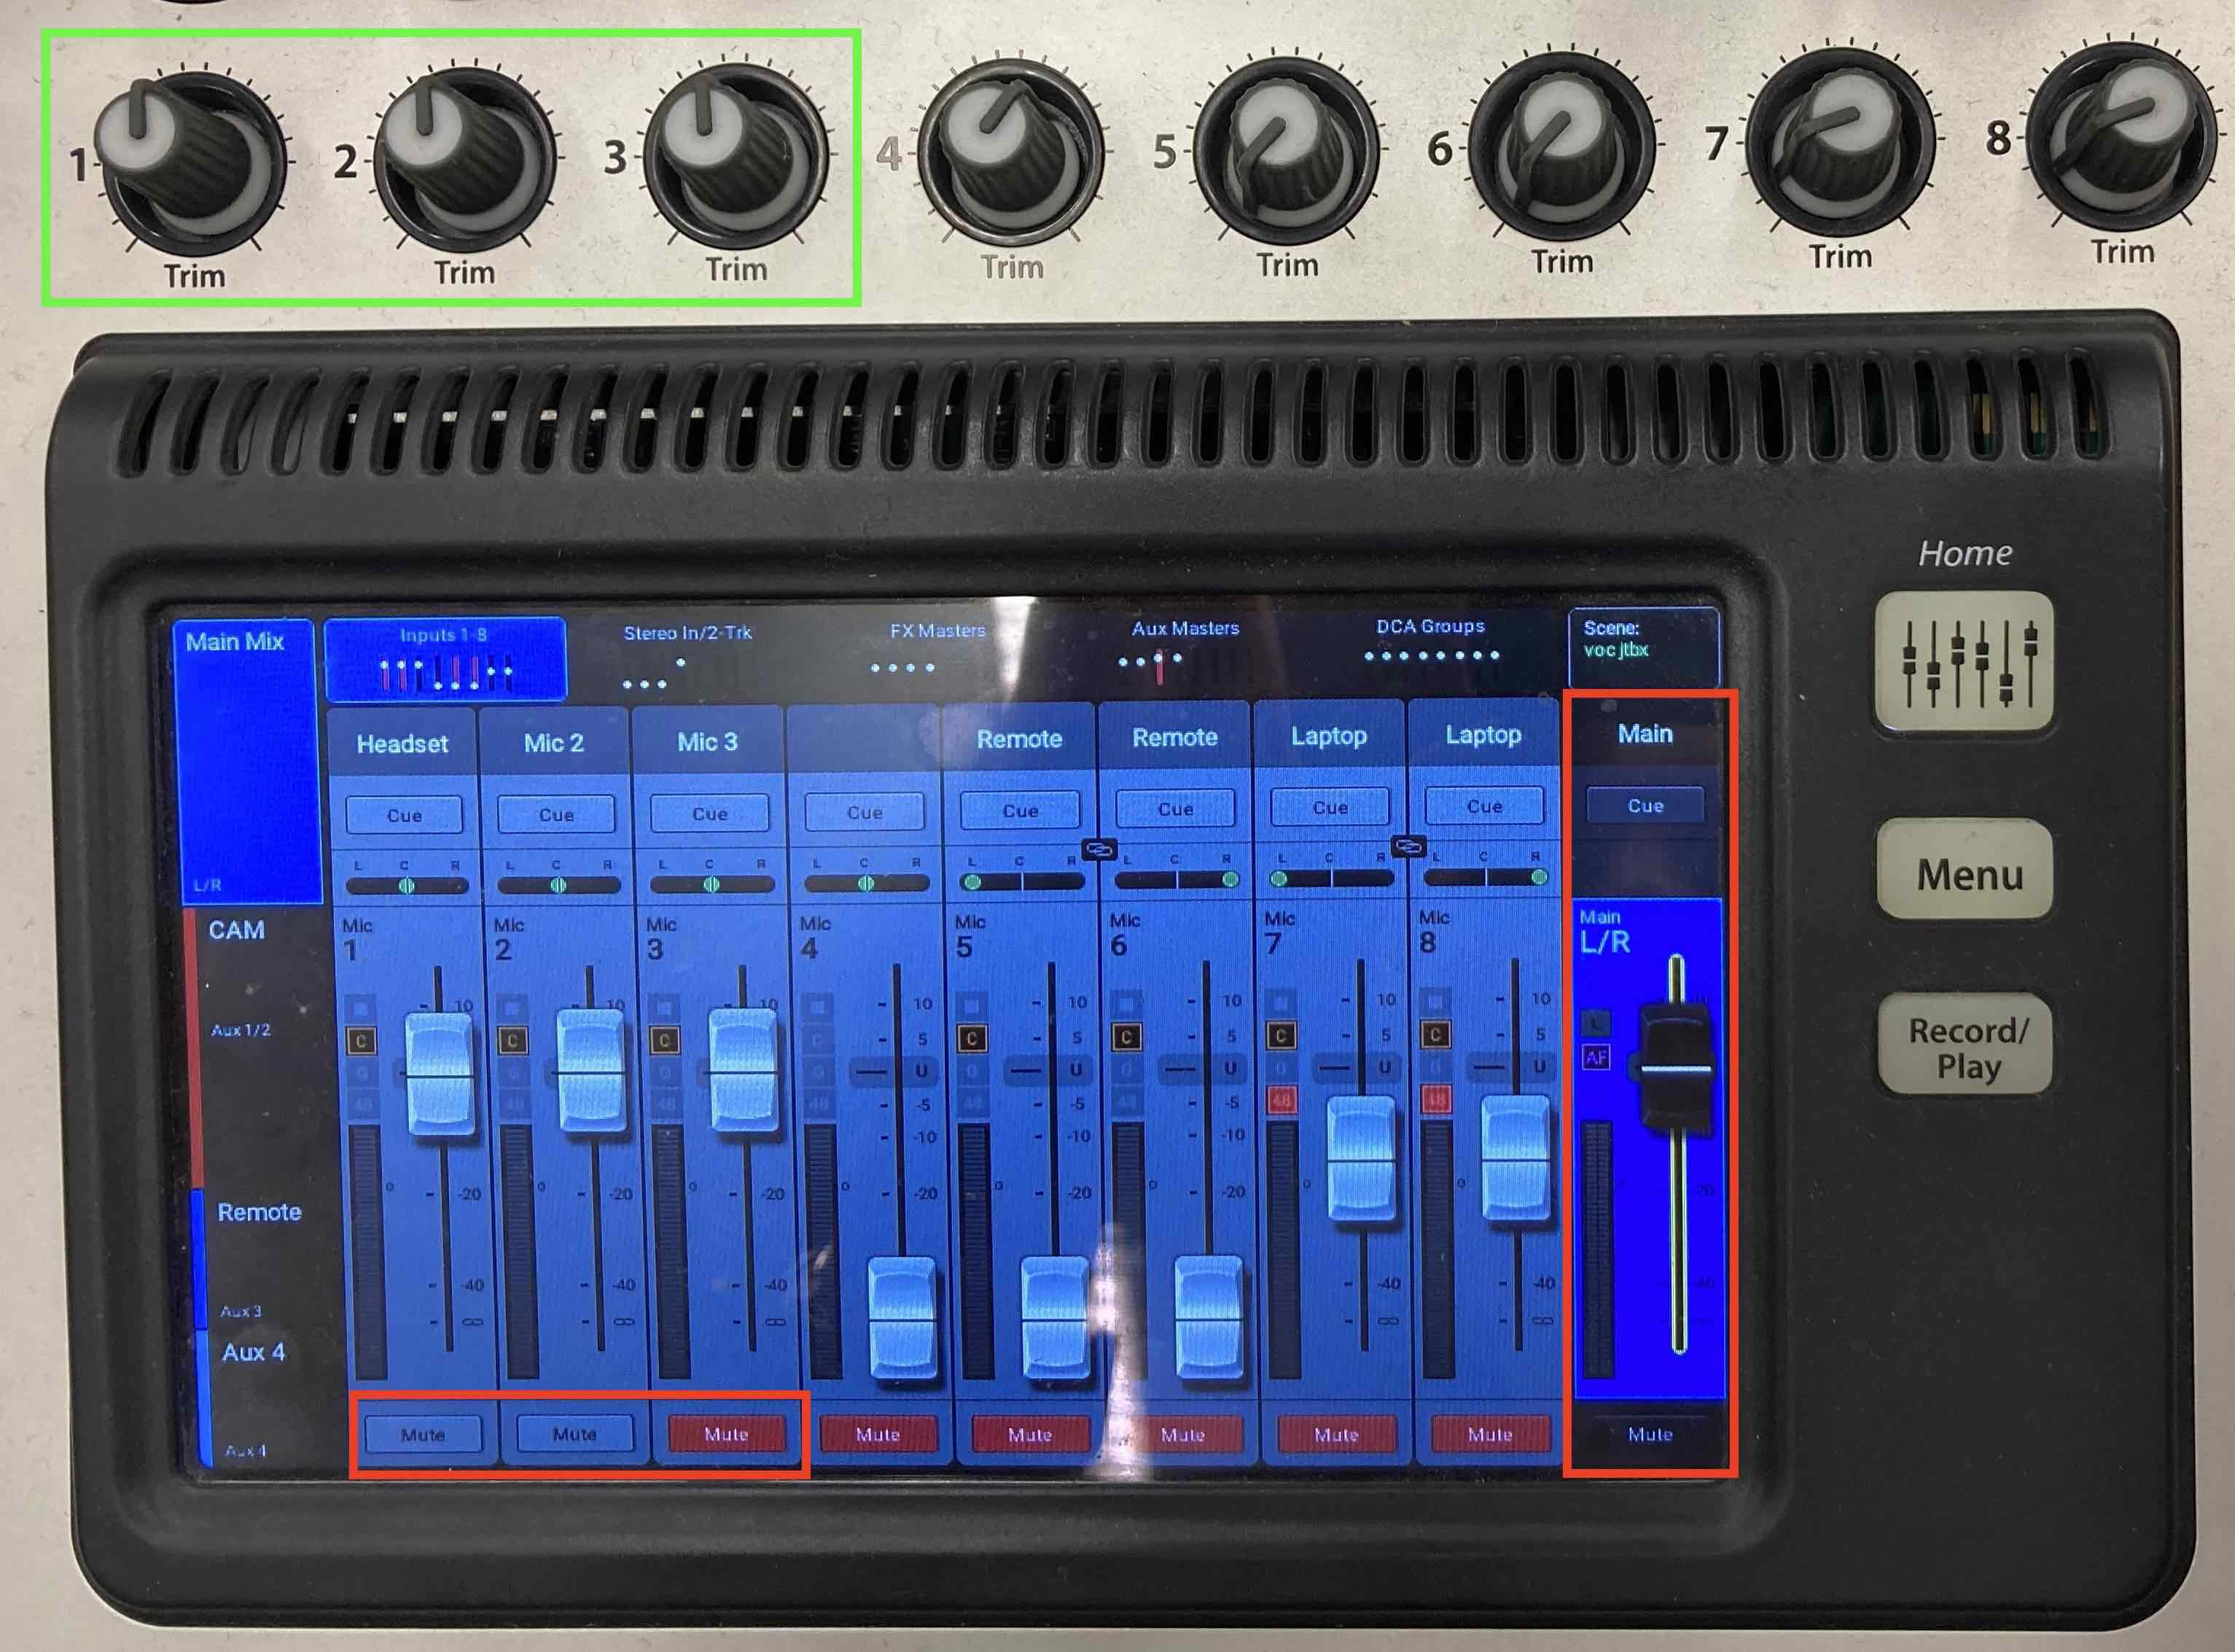
\includegraphics[width=0.9\textwidth]{images/touchmix-main-controls.jpg}
			\caption{Touchmix Main Controls}
		\end{figure}
		\column{0.4\textwidth}
		\begin{itemize}
			\item Mute unused microphones (bottom row)
			\item Adjust hall loudness with rightmost fader
			\item Adjust individual microphone level with fader or reduce "trim" knob when it's clipping
			\item Please keep microphones un-muted during applause
		\end{itemize}
	\end{columns}
\end{frame}

\begin{frame}{Audio Mixer Controls: Second Page}
	\begin{columns}[T,onlytextwidth]
		\column{0.6\textwidth}
		\begin{figure} 
			\centering
			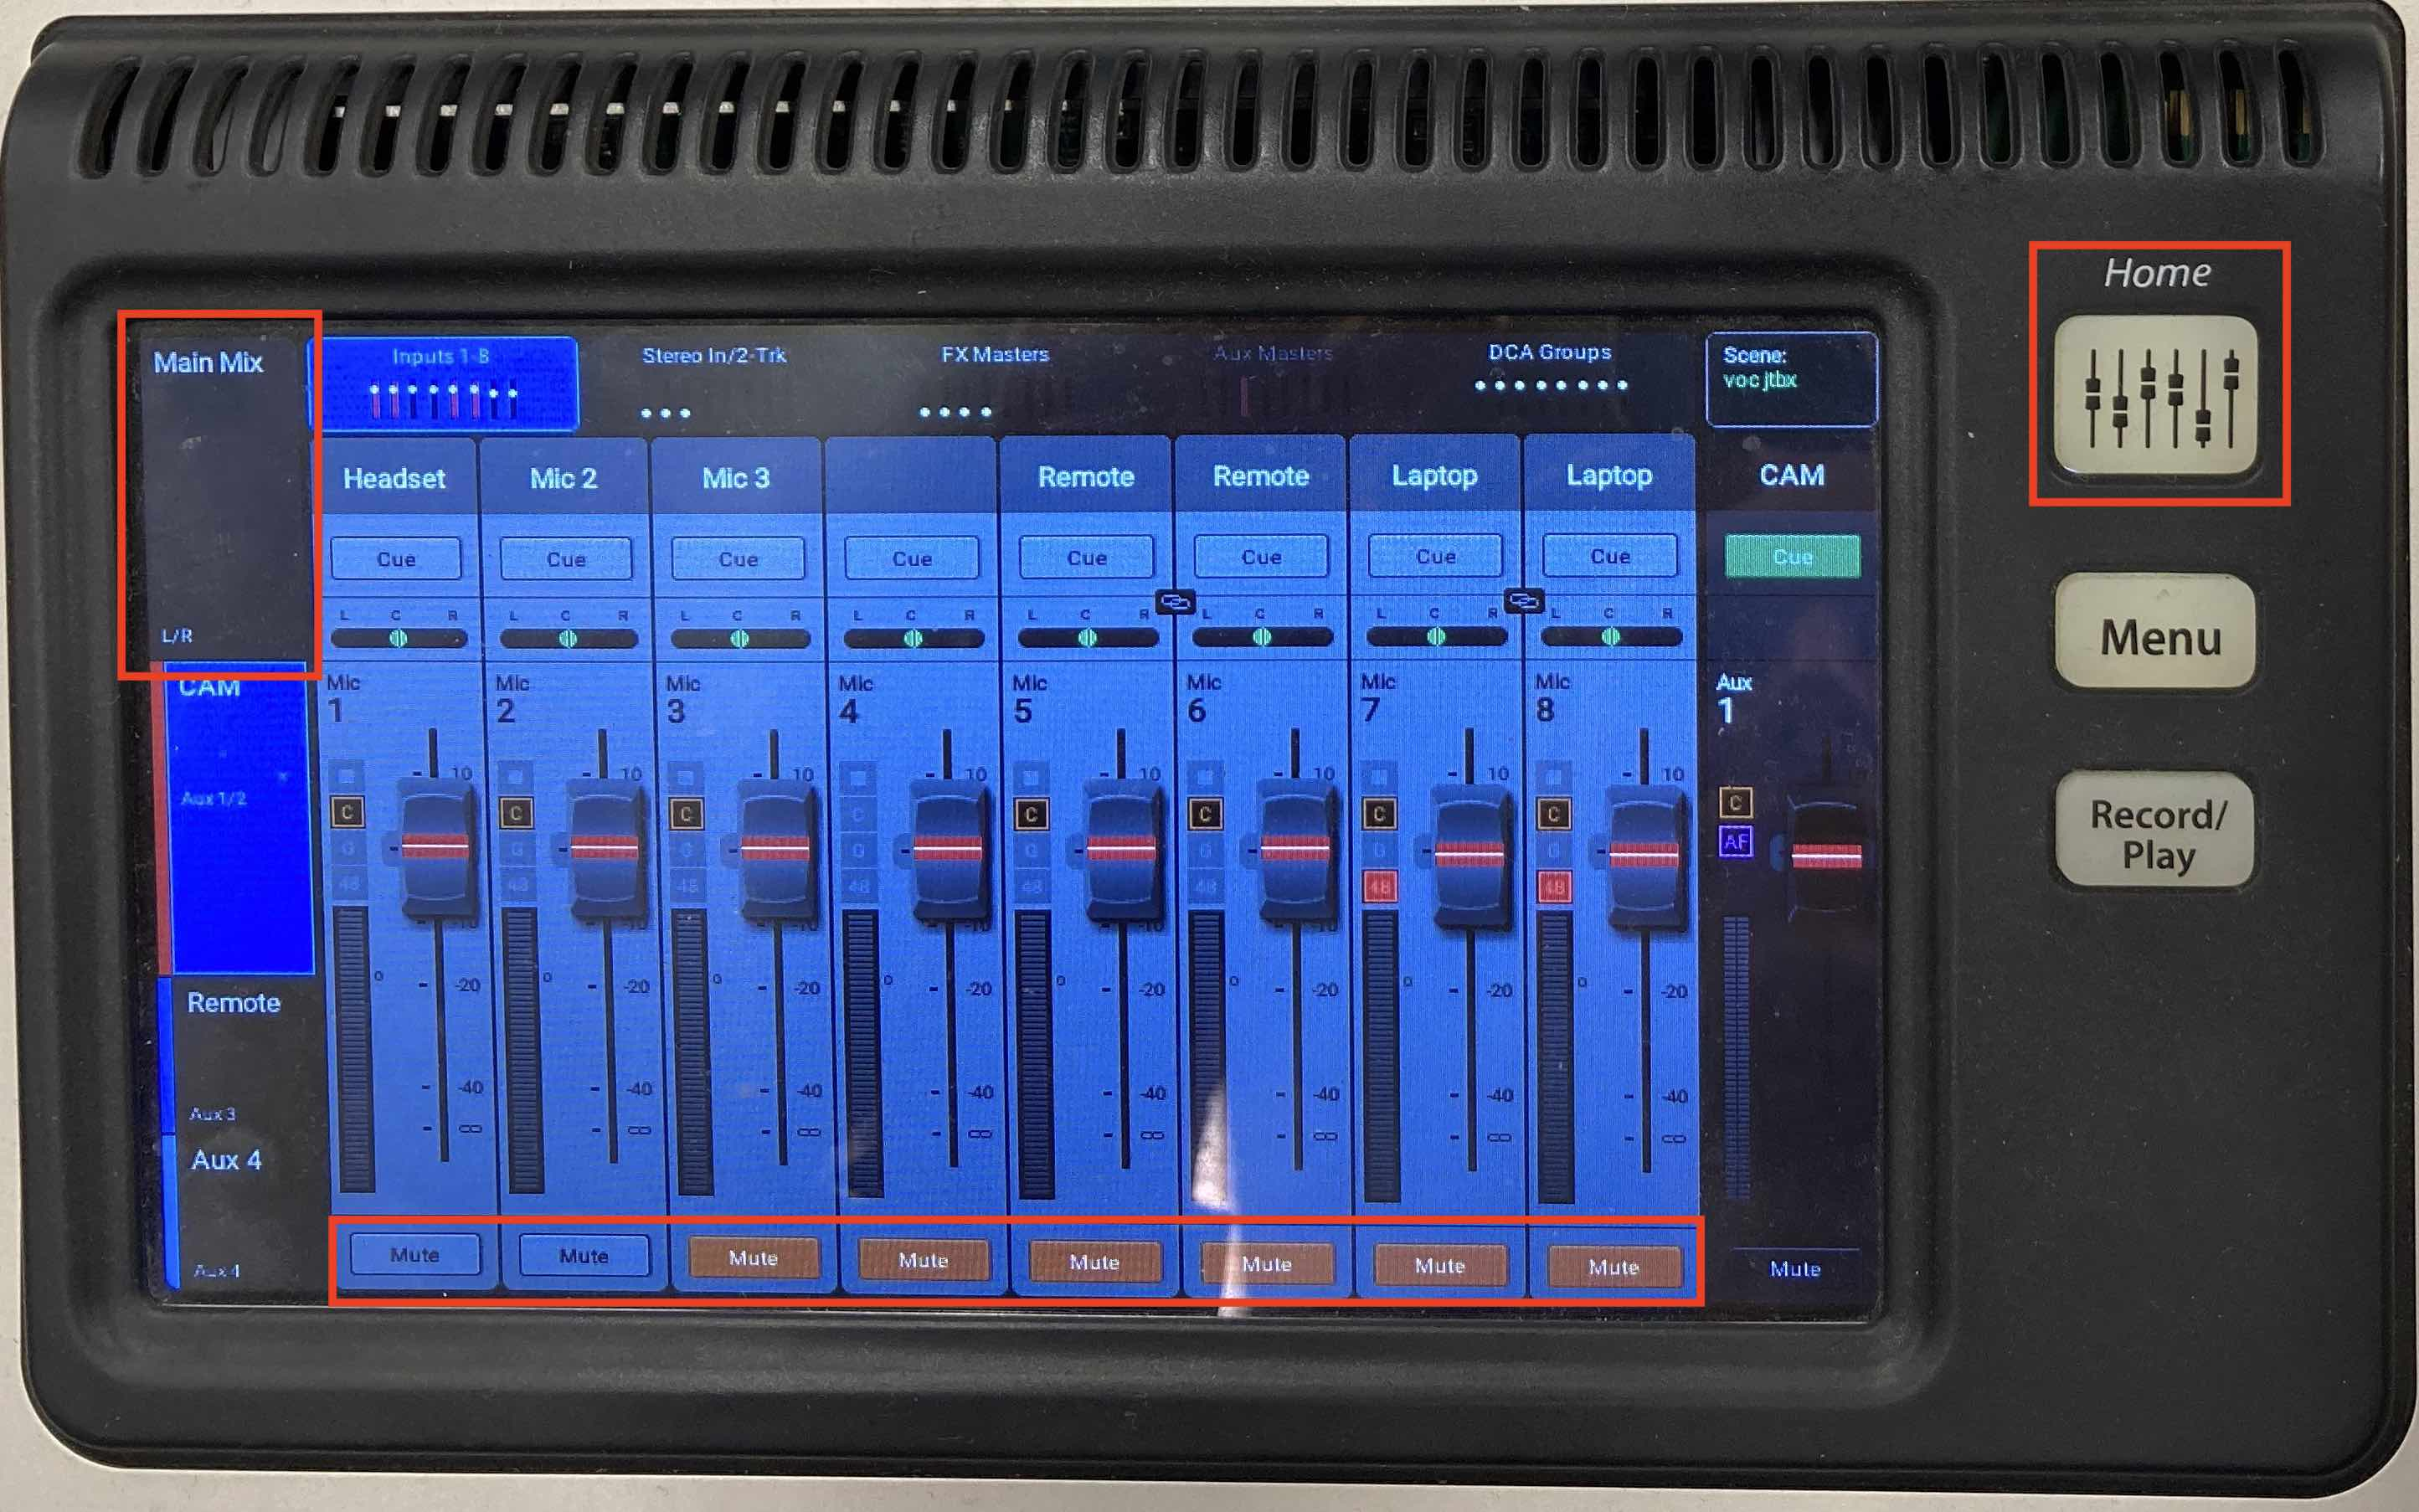
\includegraphics[width=0.9\textwidth]{images/touchmix-cam-controls.jpeg}
			\caption{Touchmix Second Page}
		\end{figure}
		\column{0.4\textwidth}
		\begin{itemize}
			\item If mute buttons are yellow, go back to "Main Mix" page
			\item If anything else is shown, just press "Home" button
		\end{itemize}
	\end{columns}
\end{frame}

\begin{frame}{Audio Mixer Controls: Headphones}
	\begin{columns}[T,onlytextwidth]
		\column{0.6\textwidth}
		\begin{figure} 
			\centering
			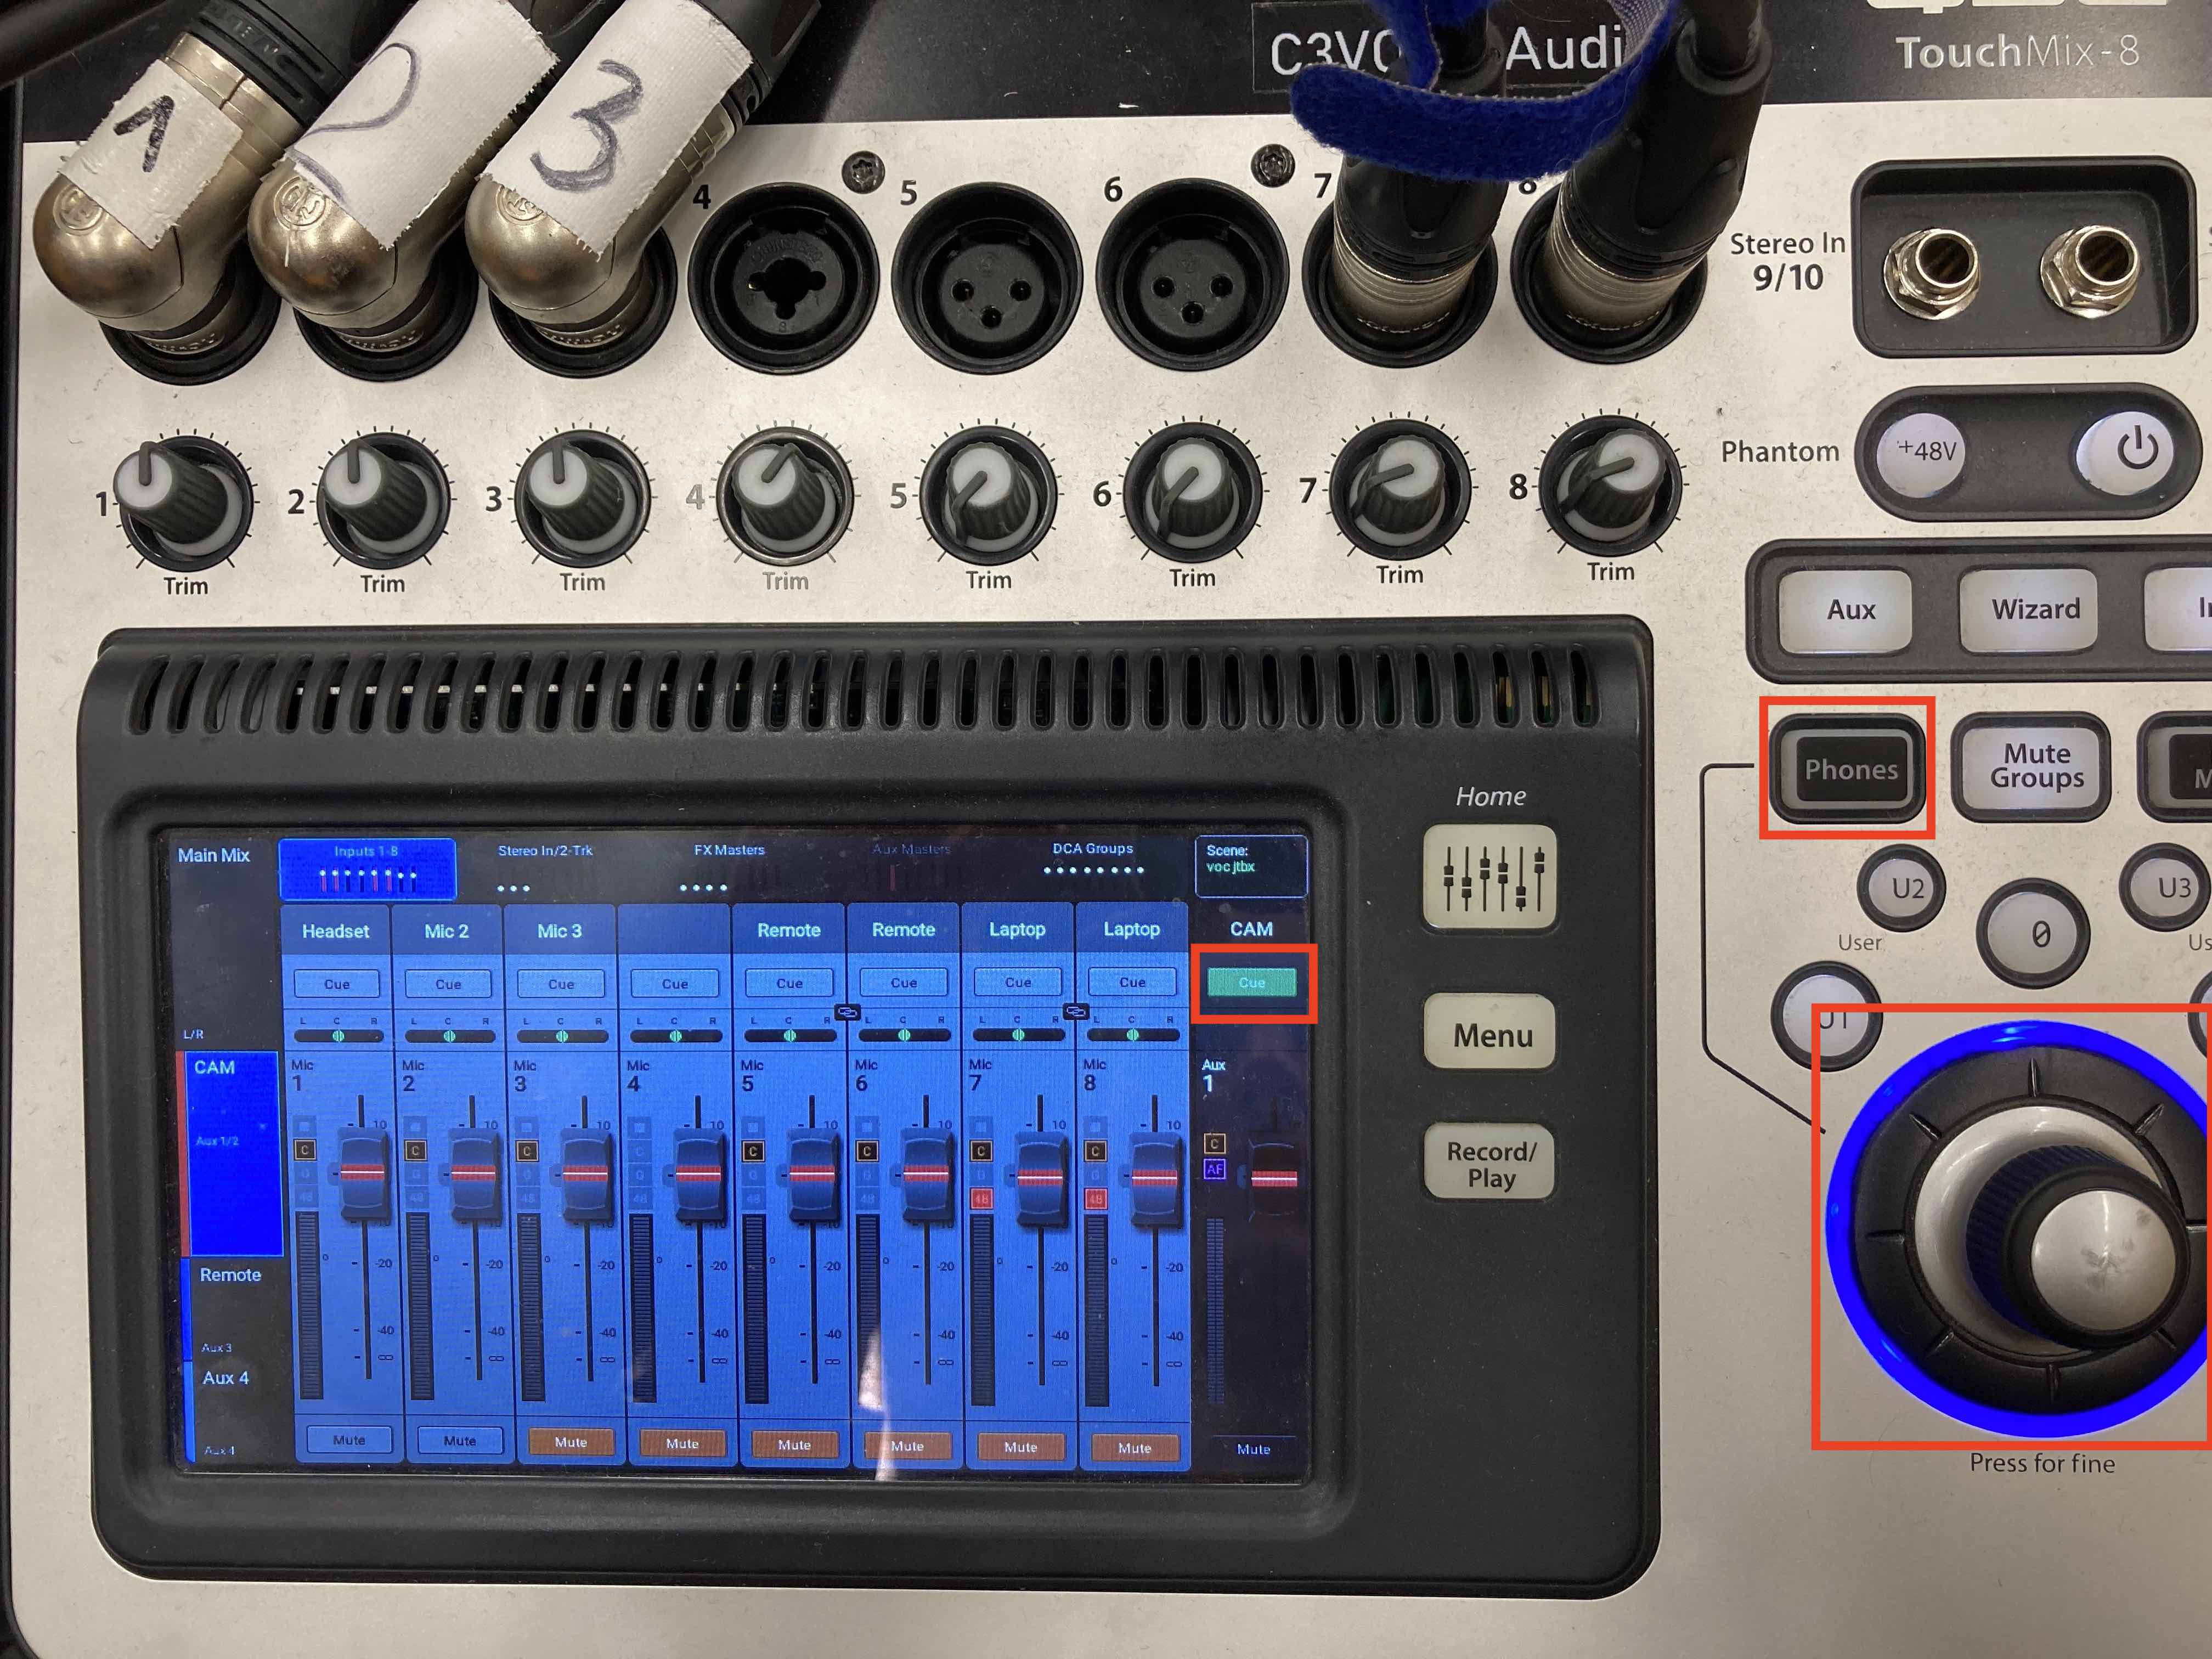
\includegraphics[width=0.9\textwidth]{images/touchmix-cam-headphones.jpg}
			\caption{Touchmix Headphones}
		\end{figure}
		\column{0.4\textwidth}
		\begin{itemize}
			\item Press "Phones" to adjust headphone loudness
			\item "Cue" on Camera/ Recoding mix must be selected
			\item Rotary knob can be used to adjust selected parameter (headphone level, channel level, etc.)
		\end{itemize}
	\end{columns}
\end{frame}

% !TEX root = ../main.tex

\begin{frame}{Audio Mixer Controls: Layers}
	\begin{columns}[T,onlytextwidth]
		\column{0.6\textwidth}
		\begin{figure} 
			\centering
			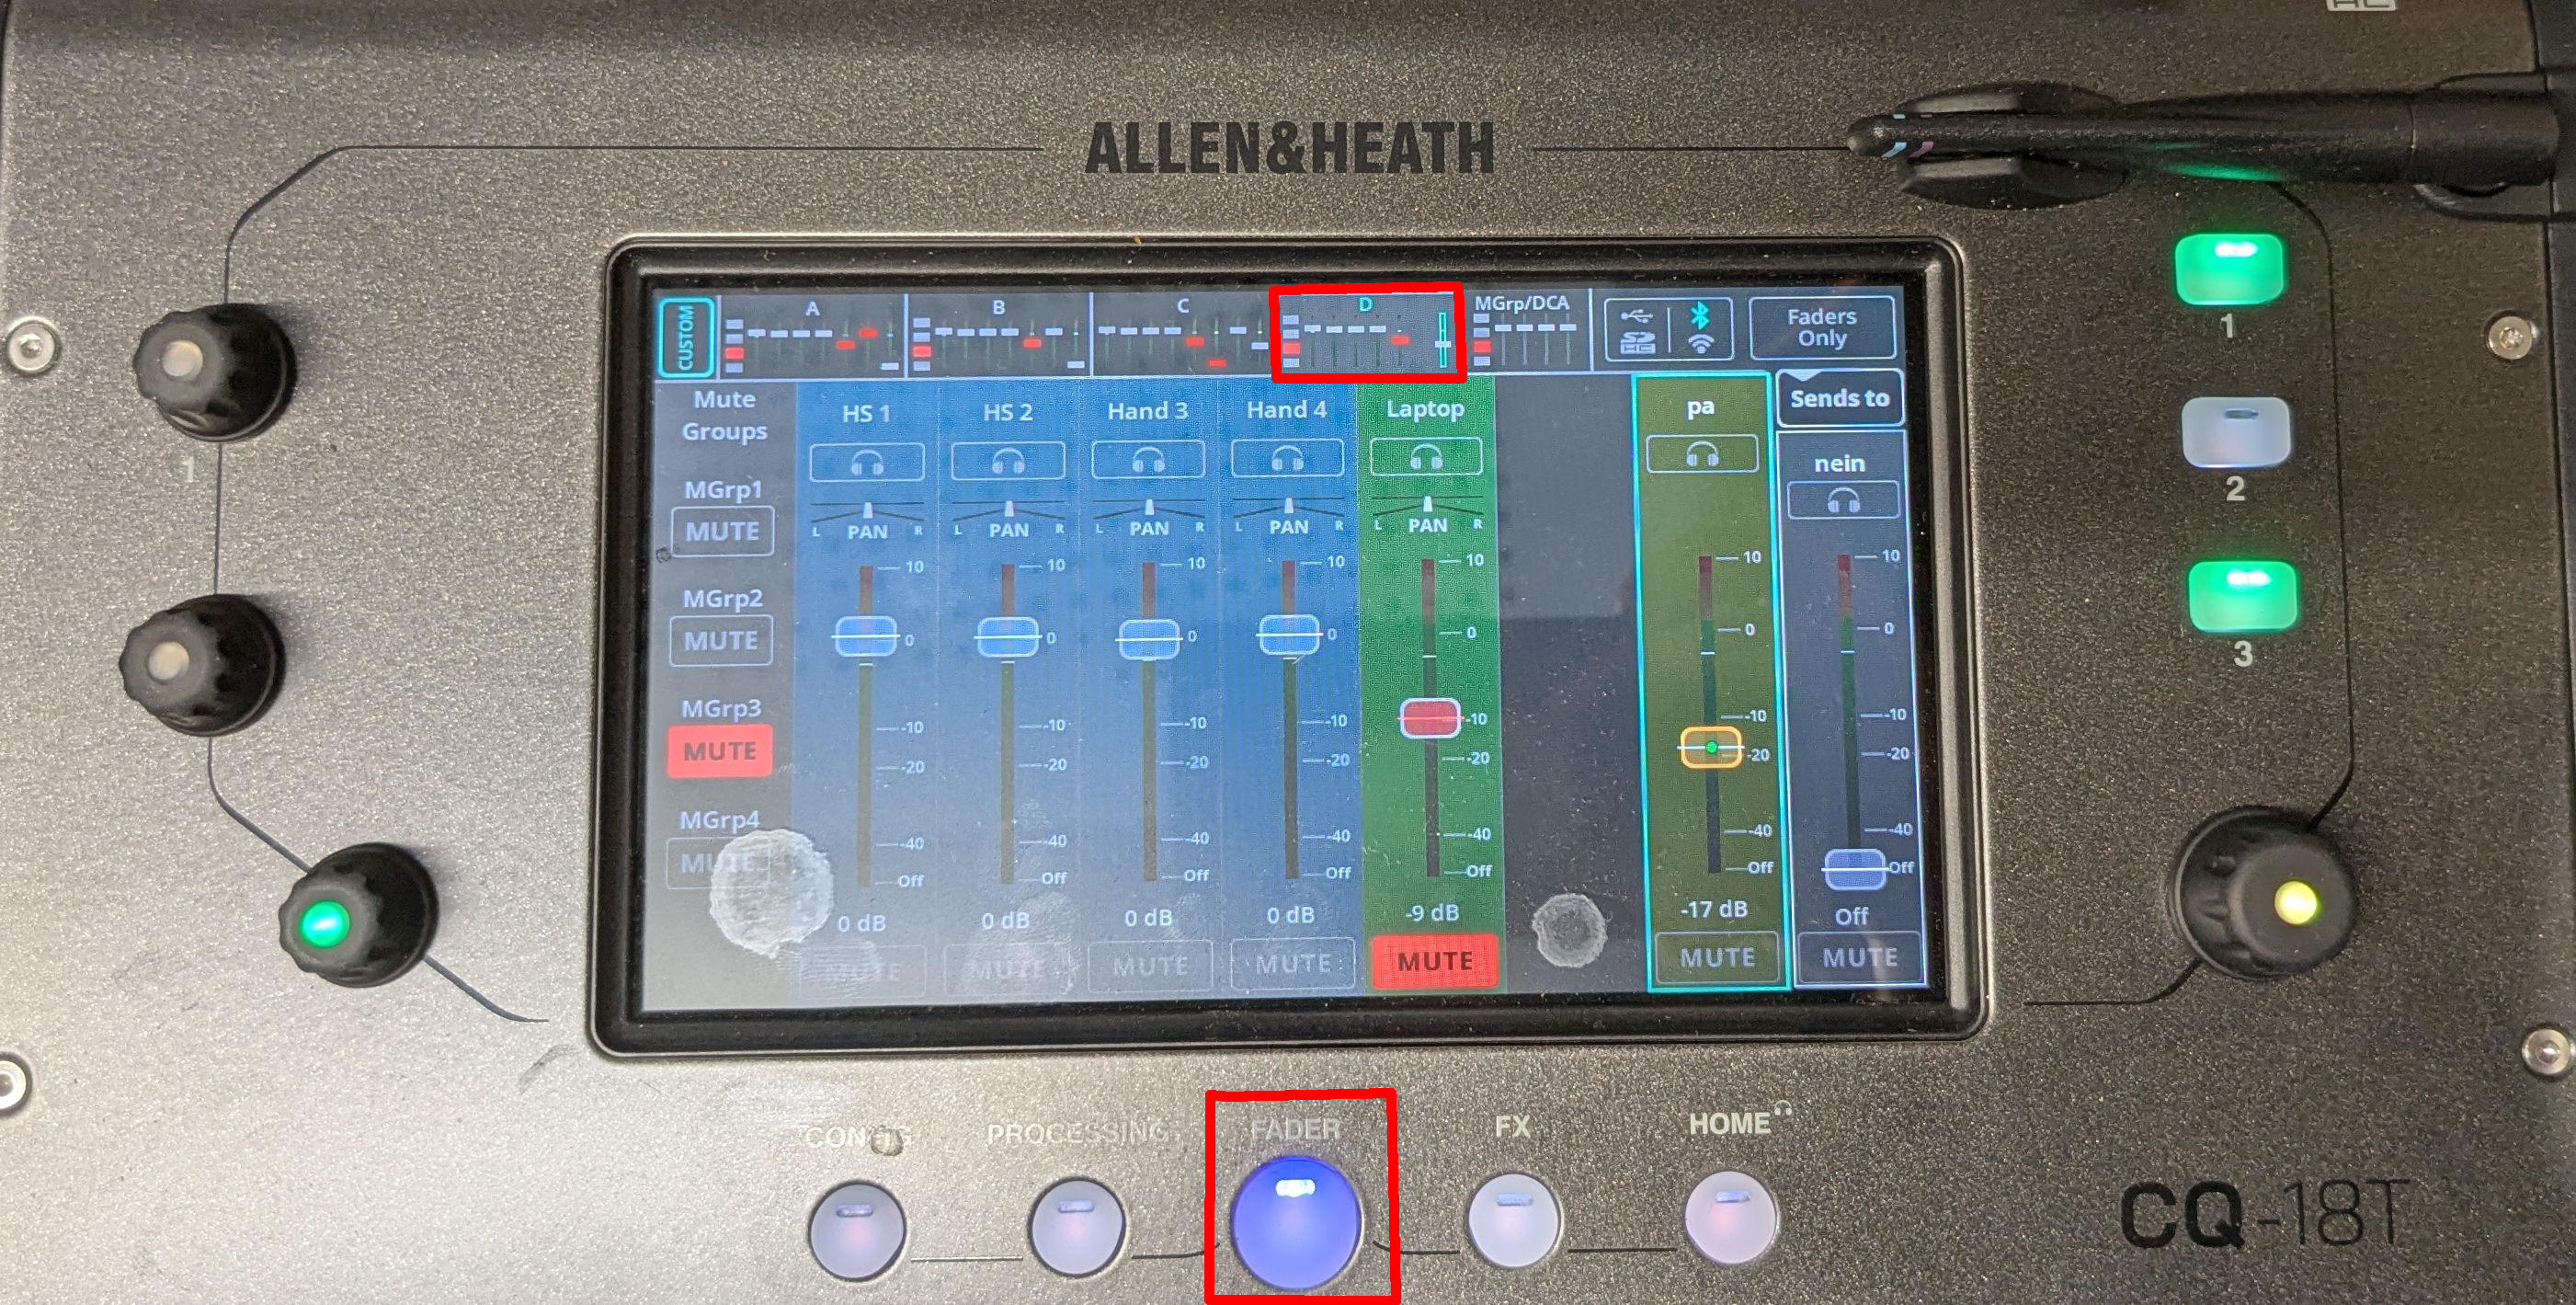
\includegraphics[width=0.9\textwidth]{images/allenheath-layers.jpg}
			\caption{Allen \& Heath CQ18T Layers}
		\end{figure}
		\column{0.4\textwidth}
		\begin{itemize}
			\item Please make sure, to always work on "Custom Workbench D"
			\item If anything else is shown, contact VOC or A/V-Technician before the talk
		\end{itemize}
	\end{columns}
\end{frame}

\begin{frame}{Audio Mixer Controls: Levels}
	\begin{columns}[T,onlytextwidth]
		\column{0.6\textwidth}
		\begin{figure} 
			\centering
			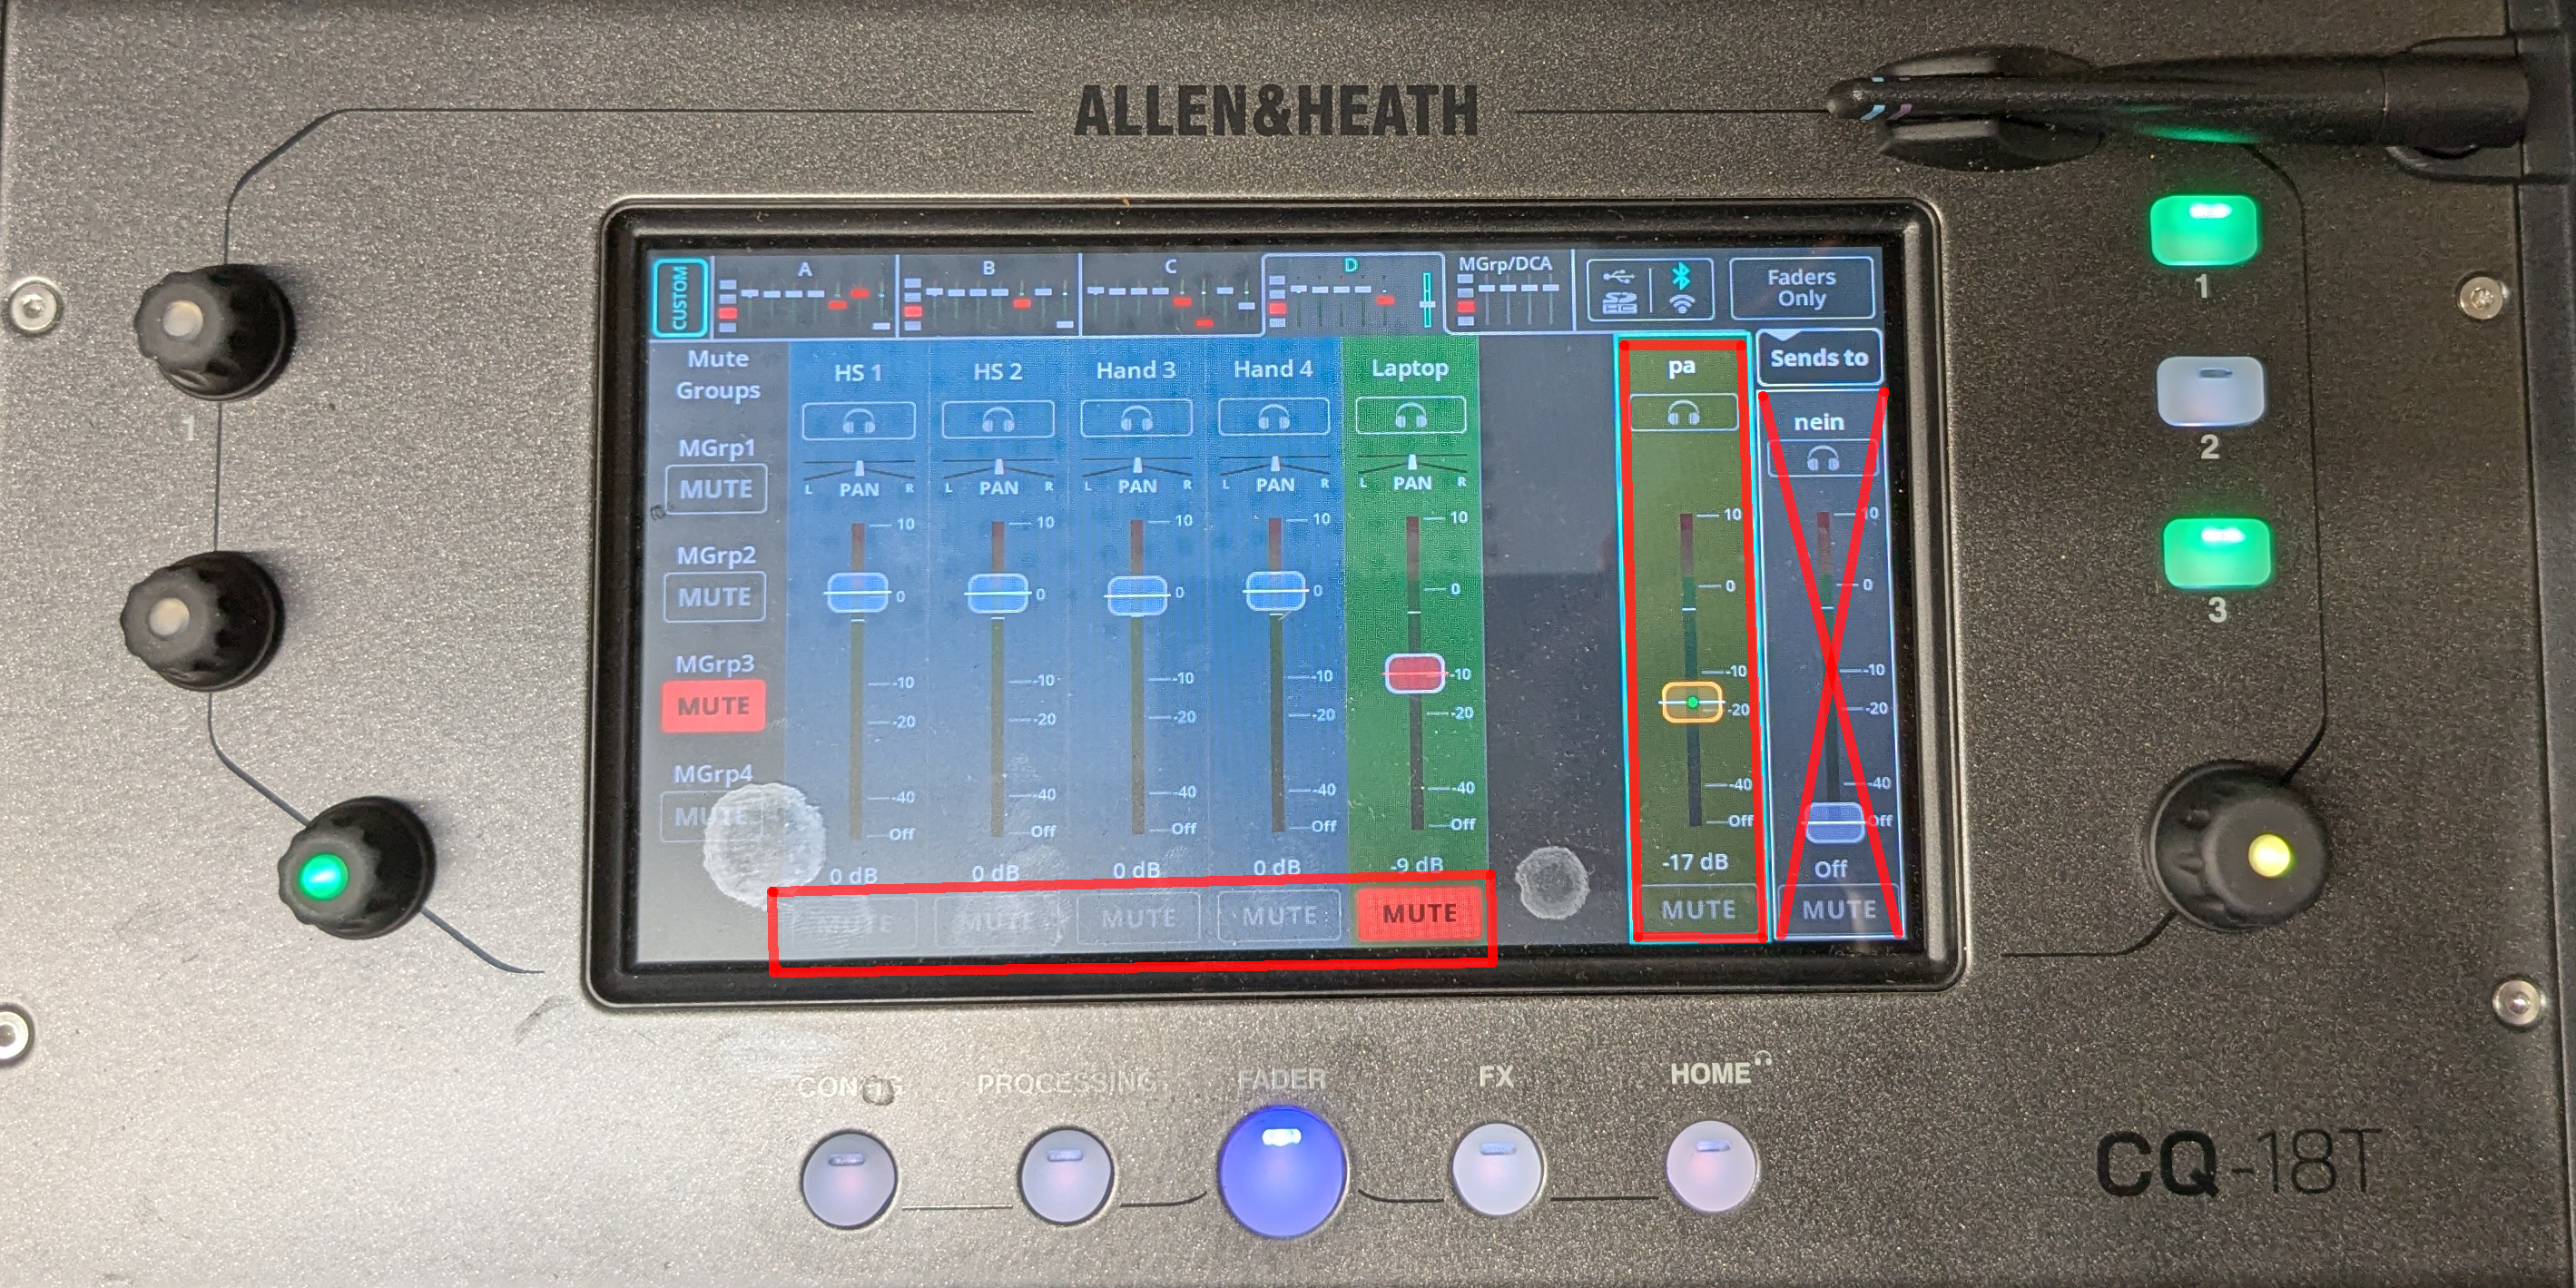
\includegraphics[width=0.9\textwidth]{images/allenheath-main-controls.jpg}
			\caption{Allen \& Heath CQ18T Main Controls}
		\end{figure}
		\column{0.4\textwidth}
		\begin{itemize}
			\item Mute unused microphones (bottom row)
			\item Adjust hall loudness with fader labeled "PA"
			\item Do not use the fader labeled "NEIN"
			\item Please keep microphones un-muted during applause
		\end{itemize}
	\end{columns}
\end{frame}

% !TEX root = ../main.tex

\begin{frame}{Microphones}
	\begin{itemize}
		\item We prefer headset microphones over handheld for speakers
		\item Distance to mouth will be constant -> more consistent audio level
		\item Handheld microphones for heralds and Q\&A
		\item Our transmitters also have a mute button (yellow light = muted)
		\item Please check battery level from time to time
	\end{itemize}
\end{frame}

\begin{frame}{Headset Placement}
	\begin{columns}[T,onlytextwidth]
		\column{0.6\textwidth}
		\begin{figure} 
			\centering
			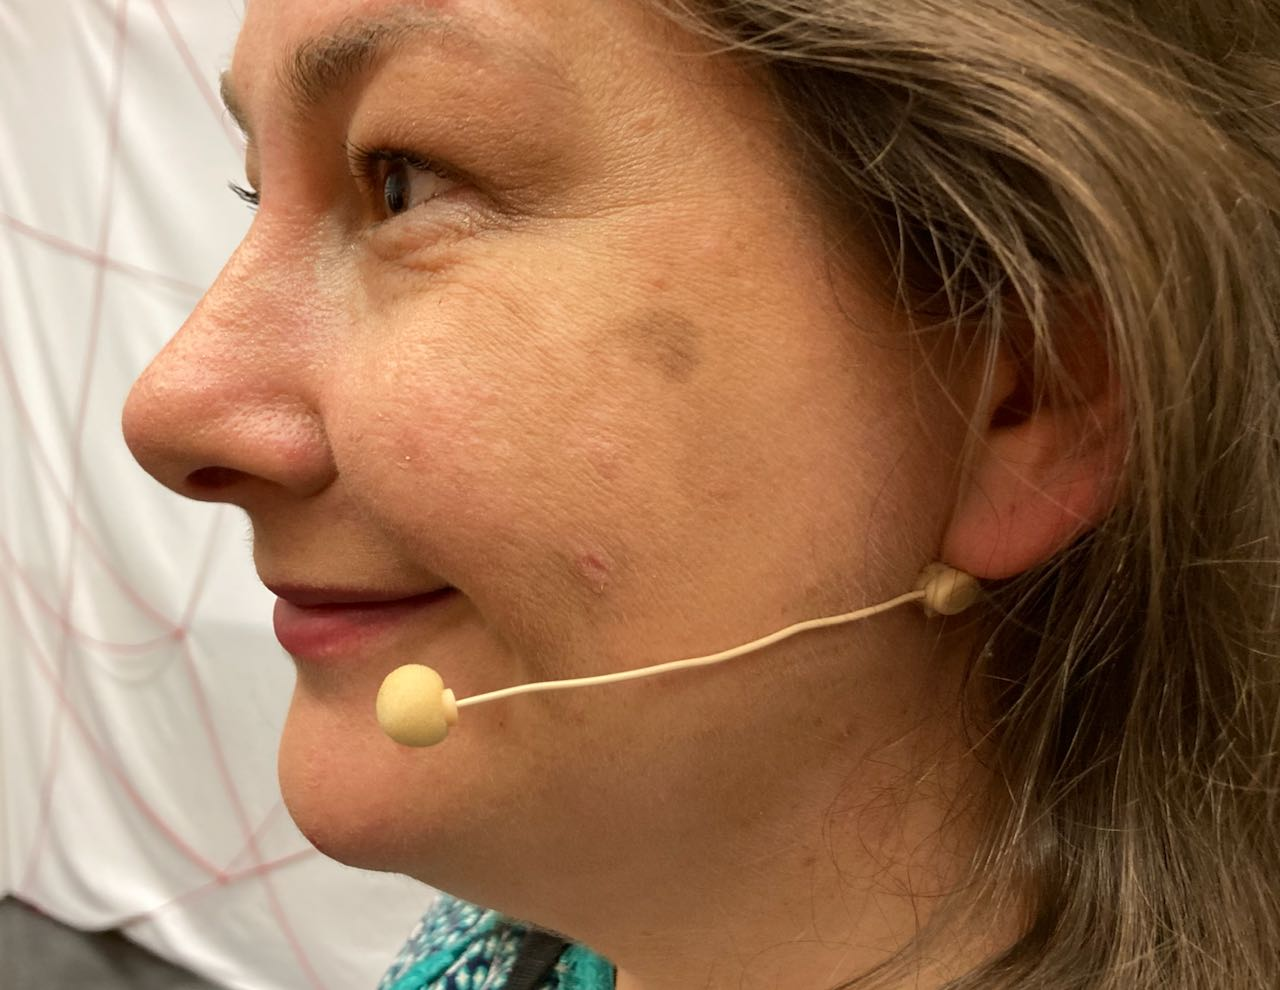
\includegraphics[width=0.9\textwidth]{images/headset-side.jpeg}
			\caption{Good headset microphone placement}
		\end{figure}
		\column{0.4\textwidth}
		\begin{itemize}
			\item Microphone shall be at the corner of the mouth
			\item Boom can slide back and forth
			\item If too far in front, there will be too much wind noise
			\item Distance to face: About 2 cm
			\item Bend boom carefully
		\end{itemize}
	\end{columns}
\end{frame}



\section{Contacts and Action Items}
% !TEX root = ../main.tex

\begin{frame}{Who to Contact?}
	\begin{itemize}
		\item Generic Questions? Something is wrong in lecture hall?
		\begin{itemize}
			\item Reach A/V Technician on duty
			\item Call the C3VOC Helpdesk \textbf{DECT 1601}
		\end{itemize}
		\item Do you want to talk to us? Come to the C3VOC Office
	\end{itemize}
\end{frame}

%% !TEX root = ../main.tex

\begin{frame}{Who to Contact?}
	\begin{itemize}
		\item Generic Questions? Something is wrong in lecture hall?
		\begin{itemize}
			\item Reach A/V Technician on duty
			\item Call the C3VOC Helpdesk \textbf{DECT 1601}
		\end{itemize}
		\item Orga-Issues? Troubleshooting? Issues with shifts?
		\begin{itemize}
			\item Call Saal Coordination \textbf{DECT 1500}
			\item non urgent issues via e-mail: saal-coordination@cccv.de 
		\end{itemize}
		\item General Angel Topics - Heaven - DECT \textbf{1023}
		\item We might need to call you. Please have your DECT number in the Engelsystem!
	\end{itemize}
\end{frame}

%% !TEX root = ../main.tex

\begin{frame}{Daily Video Mixer Shift Distribution}
	\begin{itemize}
		\item Video mixer shifts are distributed \textbf{every day at 18:00 in Hall 6}
		% \item If you can, you should attend to this meeting.
		% \item We'll distribute information and news there, e.g. if there are any special talks with additional requirements.
		\item Also this meeting should give you the chance of giving each other feedback, ask questions or rise issues.
	\end{itemize}
\end{frame}


\begin{frame}{Final Notes}
	\begin{itemize}
		\item Click "join" on the angel types you want to have
		\item Queue up to get approved
		\item Select shifts:
		\begin{itemize}
			\item Fill talks with no angels first
			\item Take breaks
		\end{itemize}
	\end{itemize}
\end{frame}

% !TEX root = ../main.tex

\begin{frame}{New Hardware}
	\begin{itemize}
		\item We have new cameras (Sony PXW-Z200)
		\item We have new audio mixers (A\&H CQ-18T) and microphones (Shure SLX-D) except from room Saal 8
		\item Lectern Module: Same ATEM Mini as before, but in a fixed casing
		\item In Hall 4 - we are testing auto-tracking of the speaker - please talk to your A/V tech how to disable it in case of emergency.
	\end{itemize}
\end{frame}

\begin{frame}{Notes for Setup at FrOSCon 2025}
       \begin{figure}
                \centering
	        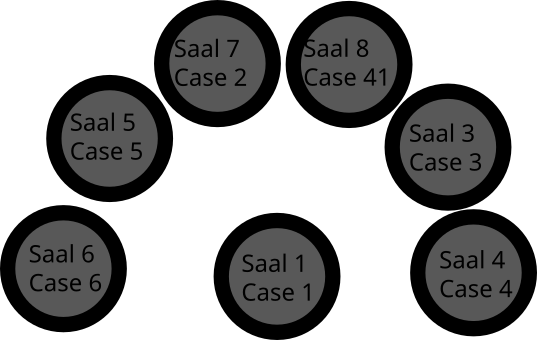
\includegraphics[width=0.7\textwidth]{images/froscon-saal-setup.png}
	        \caption{FrOSCon 2025 - Halls}
       \end{figure}
\end{frame}

\begin{frame}{Managing for happiness - trust based angel system}
	\begin{itemize}
		\item We trust you. Trust-based angel system =)
	        \item Call us @ 1600 if in need.
		\item Ask A/V tech if in need.
	\end{itemize}
\end{frame}



\begin{frame}{Angel Introduction: Questions?}
        \begin{figure} 
        	\centering
        	
\includegraphics[width=0.4\textwidth]{images/link-repo-qr.png}
        	\caption{https://github.com/voc/engelschulung}
        \end{figure}
\end{frame}

\end{document}
